\documentclass[a4paper,11pt,titlepage]{article}


% This first part of the file is called the PREAMBLE. It includes
% customizations and command definitions. The preamble is everything

% this should stop subsubsections showing up
%\setcounter{tocdepth}{4}
\setcounter{tocdepth}{2}

\usepackage[margin=2.5cm]{geometry}  % set the margins to 2cm on all sides
\usepackage{graphicx}              % to include figures
\usepackage{amsmath}               % great math stuff
\usepackage{amsfonts}              % for blackboard bold, etc
\usepackage{amsthm}                % better theorem environments
\usepackage{wrapfig}					%allows wraping of figures in the text
\usepackage{cite}
\usepackage{bm}
\usepackage{natbib}
\usepackage{har2nat}
\usepackage{float}
%\usepackage{hyperref}

% various theorems, numbered by section

\newtheorem{thm}{Theorem}[section]
\newtheorem{lem}[thm]{Lemma}
\newtheorem{prop}[thm]{Proposition}
\newtheorem{cor}[thm]{Corollary}
\newtheorem{conj}[thm]{Conjecture}

\DeclareMathOperator{\id}{id}

\newcommand{\bd}[1]{\mathbf{#1}}  % for bolding symbols
\newcommand{\RR}{\mathbb{R}}      % for Real numbers
\newcommand{\ZZ}{\mathbb{Z}}      % for Integers
\newcommand{\col}[1]{\left[\begin{matrix} #1 \end{matrix} \right]}
\newcommand{\comb}[2]{\binom{#1^2 + #2^2}{#1+#2}}

\usepackage[nodayofweek]{datetime}
\usepackage{graphicx,subfig,listings}
\longdate

\usepackage{fancyhdr}
\pagestyle{fancyplain}
\fancyhf{}
\lhead{\fancyplain{}{Visualisation for Information -\ Sam Green}}
\rhead{\fancyplain{}{\today}}
\cfoot{\fancyplain{}{\thepage}}

\usepackage{setspace}

\usepackage{url}

\title{Visualising 
		\\\ Deep Neural Networks
		}
\author{
 \Large{--- Sam Green ---}
 \\
 \\
 \small{--- Imperial College London ---}
 \\
 \\
 \small{Supervisors: Dr William Knottenbelt and Mr Daniel `Jack' Kelly}
\thanks{Submitted in partial fulfilment of the requirements for the MSc Degree in Computing Science}
}


\begin{document}
\onehalfspacing

\maketitle

\clearpage
\clearpage

\section*{Abstract}
A package, or platform designed to help experts in gaining deeper understanding of their artificial neural network models to diagnose potentially problematic issues with their model structure. This should allow for a more rapid iteration process as the researcher seeks to converge upon a well performing model.
\clearpage

\section*{Acknowledgments}
I would like to thank my supervisors Dr. William Knottenbelt and Mr. Daniel 'Jack' Kelly for their constant optimism, support and advice, my parents for their love and support, and the Turing Lab team who kept me sane throughout this project.

\clearpage

\tableofcontents
%[subsubsectionstyle=hide]

\clearpage

\section{Introduction}

	\subsection{Motivations}
	Deep Neural Networks are machine learning algorithms that enables incredibly accurate feature learning and hierarchical feature extraction. These algorithms were first employed decades ago, however made a strong comeback to the machine learning community in 2012 when in the ImageNET competition the clear winner by an unusual margin was a DNN. Since 2012 they have seen a dramatic increase in popularity in communities as far ranging as medicine, finance and sports prediction.
\par 
However unlike some machine learning models that are widely understood, such as logistic regression techniques, no one fully understands Deep Neural Networks in their full complexity. This is a problem for novice users and experts alike, and a current trend in DNN research is to explore not only the power of what these networks can do, but how they do it.
\par
There have been many studies mathematically analysing these networks, several aiming to optimise the 'gradient descent' algorithms that are at the heart of Deep Neural Networks. However this paper is concerned less with the theoretical underpinnings of the networks, but how, in a field where there is little to base complex decisions such as parameter tuning on, does a research decide how to train their models. 
\par
This paper seeks to explore the usefulness of visualisation as a research tool. The hope is that visualisation may prove to be an effective means of exploring ones network - providing key and potentially novel insights for the researchers and practitioners currently working in the field of \textit{deep learning}.
\par
Data visualisation can be defined as the graphical display of abstract information for two purposes: data analysis and communication. Data visualisation has long been an integral tool for scientific research, constituting a powerful means to discover and understand the information available in the data and to present them to others. As we currently are in the `Big Data' era, it becomes more important to expand our capacity to process this information for analysis and communication. The main goal of visualising data is to benefit from the natural human pattern recognition ability, and apply this through interactive software for efficient exploration and communication. 
\clearpage

	\subsection{Objectives}
	The main objective is to develop a tool capable of visualising the internal changes occurring within a neural network. As with any tool there are different use cases and so the objectives of this report will be to explore a number of components:
	Generating the Training Data (Running a neural net)
Produce an easy to integrate package to the work flow
Produce a more advanced system that allows for interrogation
		\begin{itemize}
			\item \textbf{Data Generation} With the majority of papers in the neural network field publishing result figures, or basic network structures that can be particular to any one set of data. The first objective to explore visualisation as a tool for understanding these networks, is to build a neural network and have the ability to easily change and tweak parameters in a controlled manner. This should produce the required data for using data visualisation upon, a collection of different models and their outputs. 
			\item \textbf{Data Visualisation: Simple work flow integration} One of the key challenges identified in early research was to produce a tool that fits into a researchers existing work flow. The first iteration of the tool must aim to be as simple to use as possible, and provide useful feedback upon a networks ability to classify and train.
			\item \textbf{Data Visualisation: A more advance tool for exploration} Having used the simple work flow tool it's likely that the researcher will begin to spot patterns in their networks output, and unfortunately with simple methods it's difficult to interrogate these outputs in a particularly effective manner. This requires the use of an interactive tool, and so the third objective of this project is to develop an interactive web-app that allows researchers to not only visualise their data, but to interact with it as well.
		\end{itemize}

	\subsection{Contribution}
	This project contributes a new tool for academic researchers that enables them to explore the changes occurring within their neural networks at every stage of training. The first tool provides a rough-and-ready approach to \textit{looking inside the black box} and quickly making assessments whether your network is learning or not. The second tool allows researchers who want to have a closer look into their data the ability to interact with the outputs of their neural network by plotting the activations of the network using dimensionality reduction techniques and correlation mapping. This allows for a more meaningful understanding of the matrix data that is output, showing how certain input data-points get misclassified, what types of representations the networks are learning, and whether the network is learning anything useful, or simply just rotating the data (a common problem).
	
	\subsection{Report Outline}
	\textbf{Chapter 2:} Presents a short introduction to Neural Networks and Visualisation before exploring in further depth how the two fields have been combined and looks at some important issues to consider.
	\par
	\textbf{Chapter 3:} Outlines 
	\par
	\textbf{Chapter 4} 
	\par
	\textbf{Chapter 5} 
	\par
	\textbf{Chapter 6} 
	\par	
	
\clearpage

\section{Identifying the Problem}


	\subsection{Understanding Neural Networks}
		
	\subsubsection{Overview}
			In order to understand Neural Networks lets first consider the human brain, a highly advanced information processing machine composed of around ten billion neurons and their connections. Artificial Neural Networks (ANNs) are a class of machine learning algorithms that seek to adopt some of the patterns within this advanced machinery, using a combination of computational and statistical methods to automate information extraction from data and allow computers to learn in a way that mimics human learning.
			\par 
			An ANN is a collection of artificial neurons that are connected together in manor which allows them to successfully learn to process information to meet some previously defined end goal. The result of learning is that an ANN becomes a high-dimensional, non-linear, function that is capable of performing a trained task quickly when called upon. Provided with enough hidden units, it can approximate \textit{any} function. 
			\par
			ANNs have been around for a long time, and had some early successes such as when in 1989 Convolutional Networks \cite{LeCun1989}, or ConvNets, first demonstrated remarkable performance in tasks such as handwritten digit classification and face recognition. It was in 2012 however when they were put back on the machine learning map. The important leap forward came with the record breaking performance on the ImageNet classification benchmark, where the Krizhevsky ConvNet achieved an error rate of almost half that of the next best rival (16.4\% in comparison to 26.1\%) \cite{Krizhevsky2012}.
			\par
			Several factors made the 2012 result possible where previously neural networks had been unsuccessful; the availability of vast training sets with millions of labelled examples, powerful GPU implementations speeding up training by great magnitudes thus enabling deeper models, and better model regularization strategies, such as Hinton's dropout \cite{Hinton2012}.
			\par 
			Since the \textit{Krizhevsky} success rapid advances in deep, or multi-layered, networks have produced significant outcomes in application areas such as vision \cite{Russakovsky2015}, speech \cite{Sutskever2014}, speech recognition \cite{Sainath2015}, NLP \cite{Norouzi2014} and  translation \cite{Graves2014}. These developments brought deep learning into the heart of the current machine learning community, which for decades had dismissed them in favour of simpler models.
\\\
\\\	

	\subsubsection{Network Structure} 

		\begin{figure}[H]
    			\centering	
    			\subfloat[Feed Forward]													{{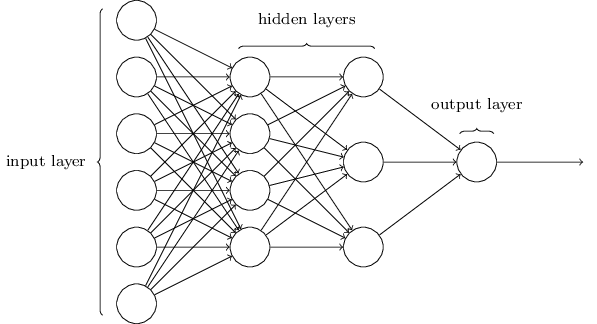
\includegraphics[width=0.25\textwidth]
    				{img/feedforward_architecture.png} 
    			}}%
    			\qquad
    			\subfloat[Convolutional]
    			{{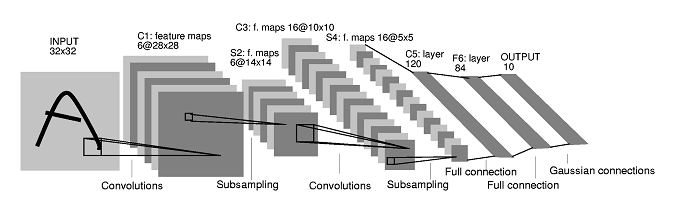
\includegraphics[width=0.45\textwidth]
    				{img/convolutional_architecture.png} 
    			}}%
    			\caption{Two of the most common architectures used for DNNs}%
    			\label{fig:architectures}
		\end{figure}		 		
		 		
		ANNs consist of a series of layers. These layers are composed of artificial `neurons' that compute a function on the inputs provided by the previous layer. They then pass the results (activations, that are typically real-valued numbers in the range [0,1]) as outputs to deeper layers. Within any individual layer there exists only one type of neuron computing the same function: these neurons are differentiated by potentially distinct inputs, outputs and weight distributions. Layers themselves are defined by the number and pattern of connections between these neurons. 
		\par 
		In order for a network to perform its task, a neural network must first be trained. This involves modifying the weights and biases of the network such that it produces the correct response for each of a number of training examples. The activations of the input units are set according to the feature values of the example, then these are propagated through the network to the output units, where the result is compared to the target output for that example and an error value calculated. This error signal is then back propagated through the network until the weights of the network have reduced the error at each node. The changes that occur are typically very small, and so large training sets are required to successfully converge the network on an optimal weight distribution. 		
		\par 
		The intuition behind back propagation, the algorithm that adjusts the weights with respect to the error value, is one of assigning 'blame'. The activations of the output nodes are determined by the activations of all the nodes below it, therefore error at the output is a result of the weights acting directly upon it from the preceding layer, and those recursively before it. In order to adjust the weights lower-down the error is backwardly propagated to the lowest hidden nodes that contributed an poor activation.		
		\par
		This process amounts to inductively learning how to solve a problem by exploiting regularities across a training set so that future similar examples may be classified in the same way. This is very similar to the way a human child learns, and again it's easy to see where these networks took some influence from.
\\\
\\\

	\subsubsection{Layers}

		\begin{figure}[H]
    			\centering	
    			{{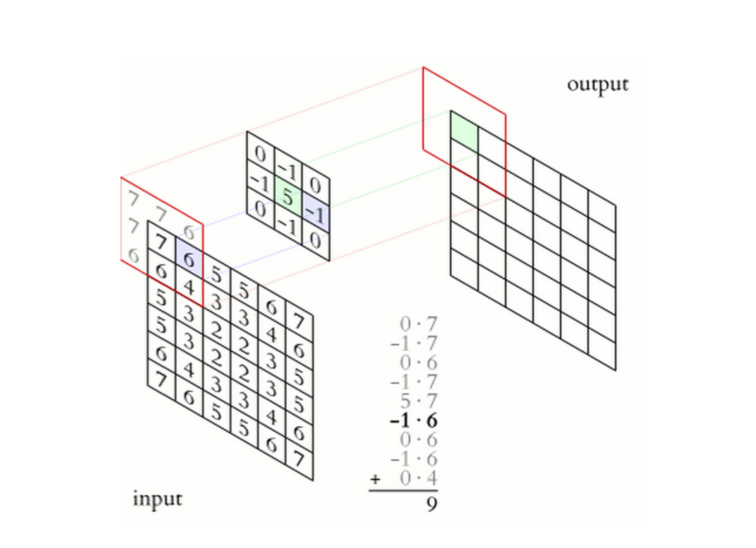
\includegraphics[width=0.45\textwidth]
    				{img/convolutional_network.png} 
    			}}%
    			\caption{Convolutional Filters}%
    			\label{fig:convfilters}
		\end{figure}		

		\par 
		There are a number of different types of layers that can be combined in a neural network: in a \textit{fully connected layer} the neurons receive an input value from every neuron in the previous layer. In a \textit{locally connected layer} the neurons are indexed spatially with inputs coming only from those nearby, and in a \textit{convolutional layer} a number of filters are applied to create a convolution. 
		\par
		The convolution of an image is produced by applying a filter upon the input image. The filter is a $k x k$ weight matrix such that $ k $ is an odd number to ensure the matrix has a true centre. The convolved image is produced pixel at a time by computing the dot product of the filter and the pixels below it, the central pixel of which is updated. A convolution is therefore produced by scanning the filter across the input pixel space until every pixel is replaced by a pixel that is some function of its filter bound neighbours. Deep successions of convolutions encode images in ways that make them invariable to translation and deformation. This is critical for classification \cite{Bruna2012}.
\\\
\\\

\subsubsection{Neurons}
		
		\begin{figure}[H]
    			\centering	
    			\subfloat[Multipolar Biological Neuron]												{{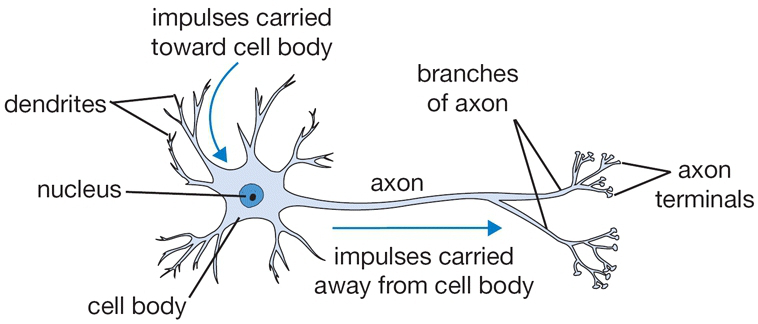
\includegraphics[width=0.3\textwidth]
    				{img/neuron_bio} 
    			}}%
    			\qquad
    			\subfloat[Artificial Neuron Model]
    			{{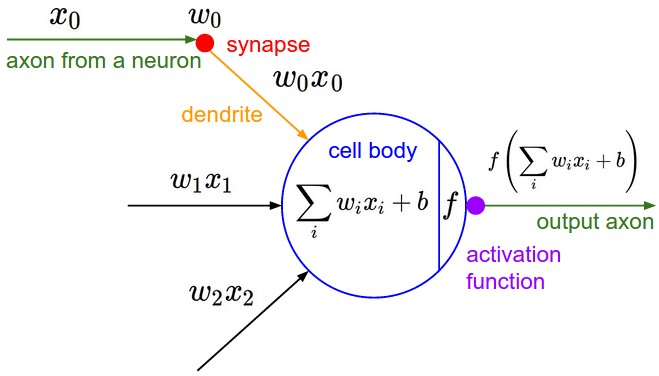
\includegraphics[width=0.3\textwidth]
    				{img/neuron_model} 
    			}}%
    			\caption{ }%
    			\label{fig:biologicalNeurons}
		\end{figure}
				
		As mentioned previously, artificial neural networks are modelled on the human brain. They take influence from the \textit{multipolar biological neuron}. The neuron receives multiple electric charges from its neighbours through the dendrites. This then triggers a single electric charge to a different set of neighbouring neurons through its axon terminals. Artificial neurons perform effectively the same task and compute functions that take in multi-dimensional input but output a mono-dimensional result.
\\\

There are a number of different neurons used within the layers of an artificial neural network:
		\\\
		
		\textbf{Binary Threshold Neuron} 
		
		$$
		y = \begin{cases}
		1 & \text{if \textit{M} $\le \sum\limits_{i=1}^k x_{i} \cdot w_{i} + b $ where \textit{M} is a threshold parameter} \\
		0 & \text{otherwise.}
		\end{cases}
		$$

		Here, \textit{y} is the output of the neuron calculated by the weighted input acting upon it, and assessing this value against some threshold \textit{M}. The threshold neuron works much like a biological neuron in that it either outputs a charge or it doesn't. This neuron however is rarely used due to the fact that it cannot be used in optimisation algorithms, such as gradient descent, which require a function to be differentiable. 
	\\\

		\textbf{Logistic Sigmoid Neuron}	
		
		$$
		y = 
		\text{ $ \frac{1}{1 + \exp (-z)} $
		, where z = $ \sum\limits_{i=1}^k x_{i} \cdot w_{i} + b $}
		$$ 
		
		A more commonly used transfer function is the sigmoid, which is an approximation of the threshold function above. Here the bias $ b $ performs a similar function to the threshold \textit{M} in the previous example. The `threshold' can be through of as the point at which the gradient of the \textit{decision surface} is steepest. While in the threshold neuron this represents a hard boundary, the sigmoid represents a gradient of values. One disadvantage of the sigmoid is that is is more expensive to compute.
		
		\begin{figure}[H]
    			\centering	
    			\subfloat[Sigmoid A]																			{{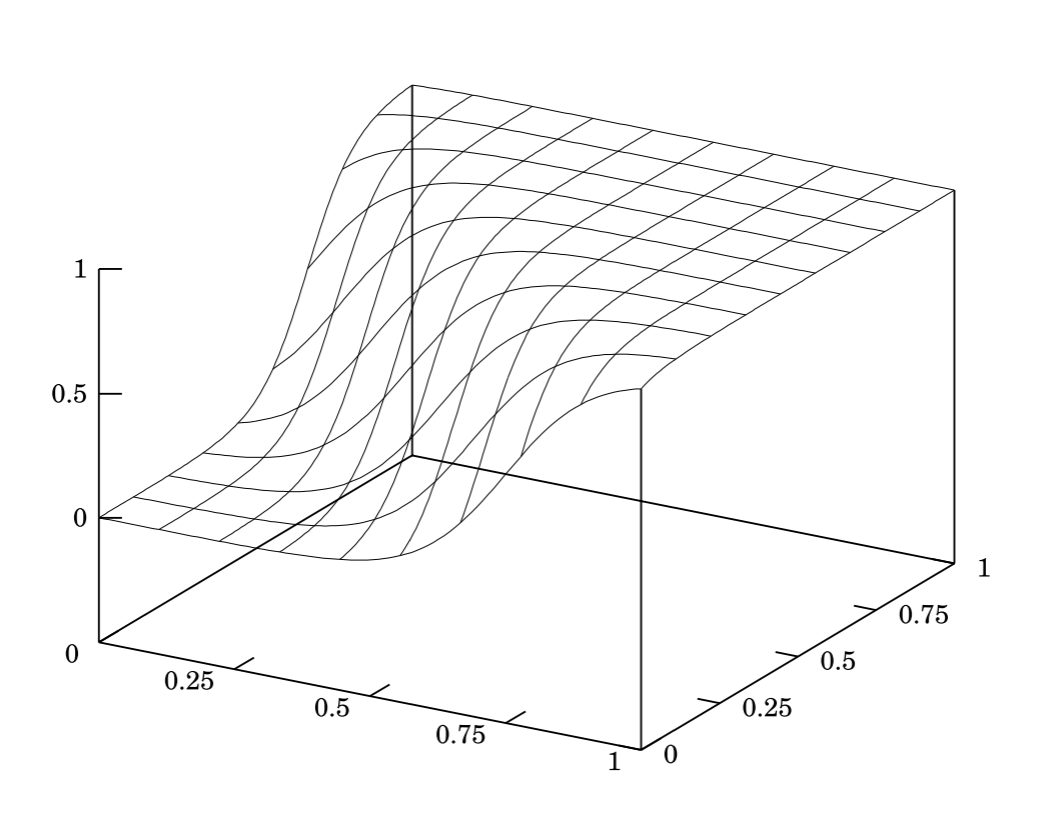
\includegraphics[width=0.2\textwidth]
    				{img/craven_sigmoid.png} 
    			}}%
    			\qquad
    			\subfloat[Threshold]																			{{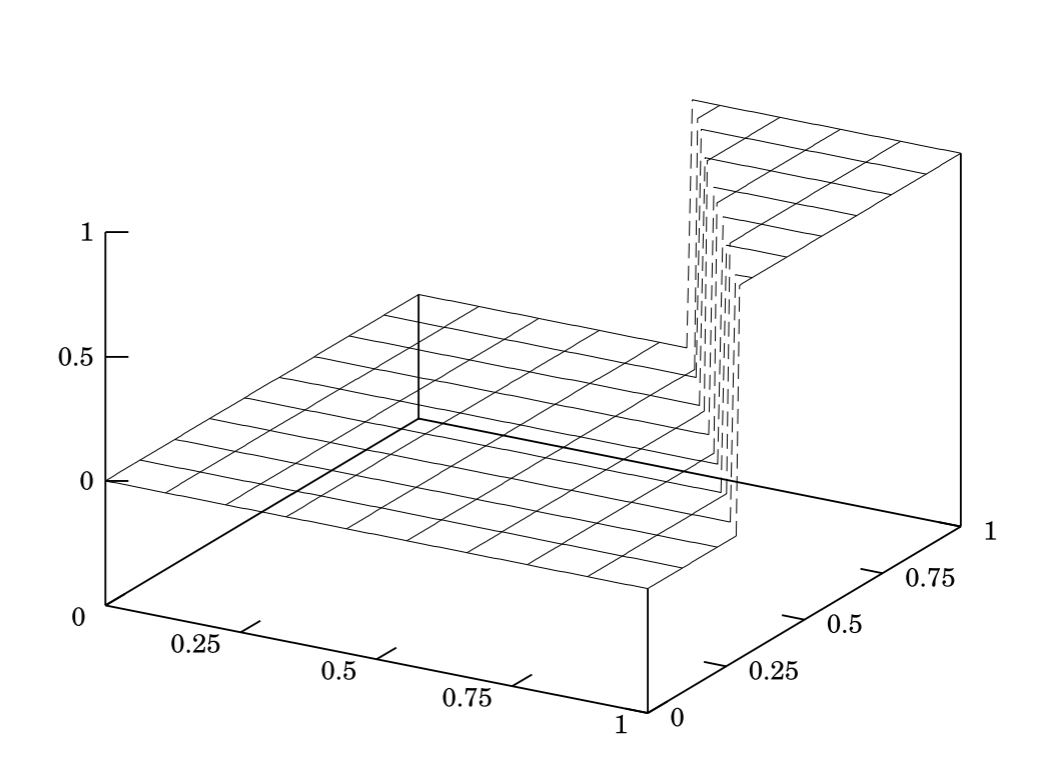
\includegraphics[width=0.2\textwidth]
    				{img/craven_threshold.png} 
    			}}%
    			\qquad
    			\subfloat[Sigmoid B]
    			{{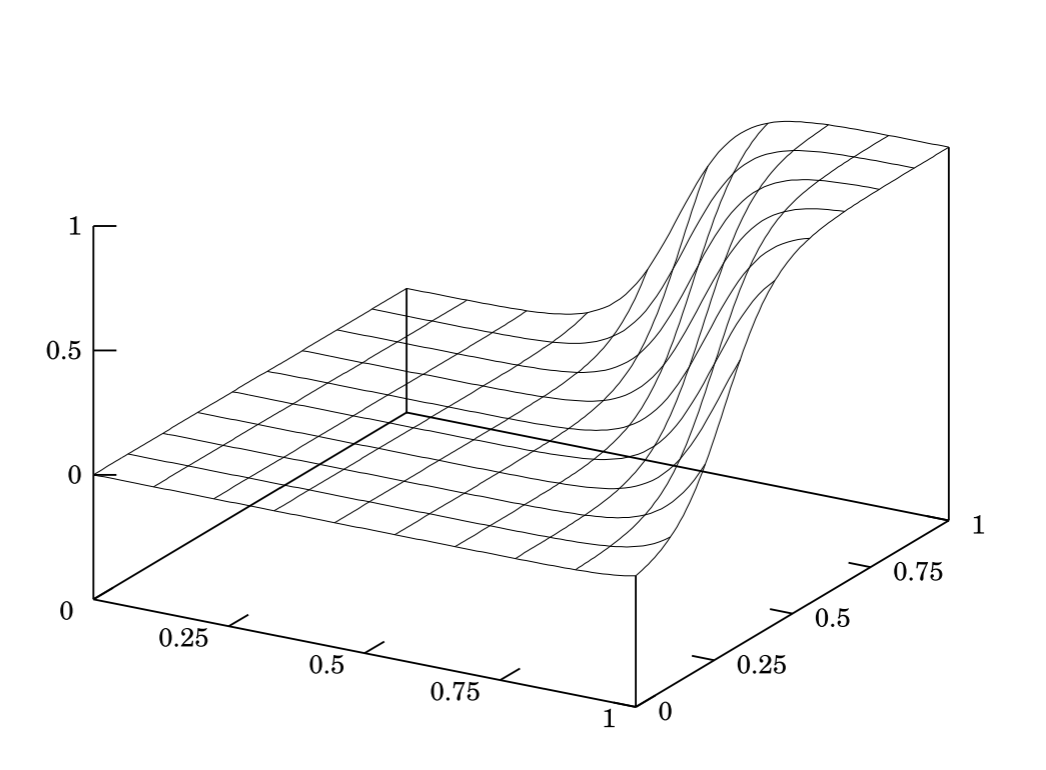
\includegraphics[width=0.2\textwidth]
    				{img/craven_sigmoid_2.png} 
    			}}%
    			\caption{}%
    			\label{fig:SigmoidNeurons}
		\end{figure}

		\textbf{Rectified Linear Neuron (ReLU) }
		
		$$
		y = 
		\text{ max$\{0,  b + \sum\limits_{i=1}^k x_{i} \cdot w_{i}\}$ }	
		$$		
		
		The rectified linear neuron is a hybrid function. It is more efficient to compute that the sigmoid neuron and is partially differentiable, thus making it suitable for gradient descent. The compromise here is the cost of sophistication of the result. The neuron introduces a non-linearity with its angular point, a smooth approximation of which is the softplus $f(x) = log(1 + e^{x}))$.
\\\
\\\

\subsubsection{Design Space}
		In a typical machine learning workflow, including working with ANNs, practitioners iteratively develop algorithms by refining choices in areas such as feature selection, sub-algorithm selection, parameter tuning and more \cite{Patel2008}. This is usually done through a trial and error approach that is perhaps similar to hill-climbing in the model space and can lead to locally minimal results. This is generally considered to be unsatisfactory due to the small number of outputs that a researcher may be following as a guideline - such as error.
						
		\begin{figure}[H]
    			\centering	
			{{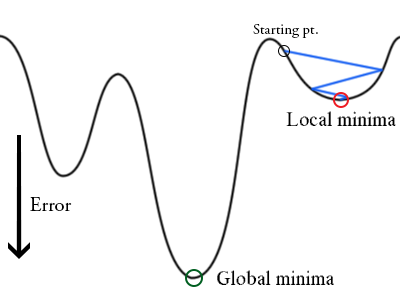
\includegraphics[width=0.3\textwidth]
    				{img/gradient_descent.png} 
    			}}%
    			\caption{Hill Climbing in the parameter space (Gradient Descent)}%
    			\label{fig:GradDesc}
		\end{figure}	
		
		\par 
		The most challenging and time-consuming part of training a neural network lies in selecting the correct parameters, of which there are many, and each affects the network in an almost unknown capacity. Some examples are:
		\par
		\textbf{Size of Filters:} if the filter is too small features will be too coarse, however if the filter is too large the complexity of a model increases significantly with little benefit.
		\par
		\textbf{Number of Layers:} additional layers tend to improve performance, however they also increase a models complexity and thus its training time - this means that fewer model iterations are possible with a set time period. Back propagation issues with layers failing to train, can also arise.
		\par 
		\textbf{Filters per Layer:} additional filters likewise tend to improve performance, and again there is likely to be a cut-off point where diminishing returns are outweighed by increased model complexity and training time.
		\par  
		\textbf{Layer Connectivity:} variations in locally-connected and fully-connected layers can change performance dramatically, such as exhibited in the difference between convolutional layers, connected layers and those with dropout.
		\par 
		\textbf{Input and Output Data Encodings:} different vector encodings change the way the network learns. Images for example with a height, width and three colours per pixel are compressed into a one-dimensional vector as an effective input encoding.
		\par  		
		\textbf{Error Space, or Bound:} changes how the network perceives error, and thus fundamentally effects what it learns during the back-propagation optimisation period.
		\par		 		
		\textbf{Initialization of Weights:} can also alter how a model learns. There are a number of different possible approaches to this: such as uniformly, randomly, as a Gaussian, unsupervised pre-training and more.
		
		\par 
		\textbf{Auxiliary Layers:} in ConvNets for example, pooling and normalization layers are often applied, however each has it's own set of additional parameters to tweak and a different effect on the model, thus requires complex tuning.
		\par 
		\textbf{Non-linear functions:} can make a large difference on model performance: the choice of which non-linearity you choose, for example choosing a 'Rectified Linear' neuron as opposed to a 'sigmoid'. 
		\par 
		\textbf{Optimization Parameters:} such as step-size, or learning rate, regularisation, mini-batch sampling all need to be tuned for maximum accuracy and convergence speed. While there are common algorithms that help choose these parameters, such as AgaGrad \cite{Duchi2011}, manual tuning is often still required, and is difficult to get right.
		\par
		\textbf{Momentum Co-efficient:} adds a fraction of the previous weight update to the current one, and is used to prevent the system from converging to a local minimum or saddle point, and increase the speed at which it converges. Too high and risk of overshooting the minimum, and too low the system might still hit a local minima.
\\\
	\subsection{Black Box Problem}
		\subsubsection{Overview}
		While there have been a number of improvements to neural networks over the years (such as the development of drop-out, or deeper architecture) they remain to be considered by many as a black box algorithm, especially in comparison to some other better studied and less complex machine learning techniques such as support vector machines or logistic regression. Indeed many popular machine learning competitions are still won by those better understood algorithms \cite{Adams2015}.
		\par 
		There is still no clear understanding of why they perform so well or why certain combinations of internal weights and connections enable highly complex tasks, such as computer vision, to be performed. It is due to this lack of understanding that the development of new models falls largely upon a `greedy' trail and error approach to tuning the network parameters. This is unsatisfactorily unscientific, using experience and intuition as the primary guiding factors - making insights hard to replicate.
		\par
		
		\begin{figure}[H]
    			\centering	
			{{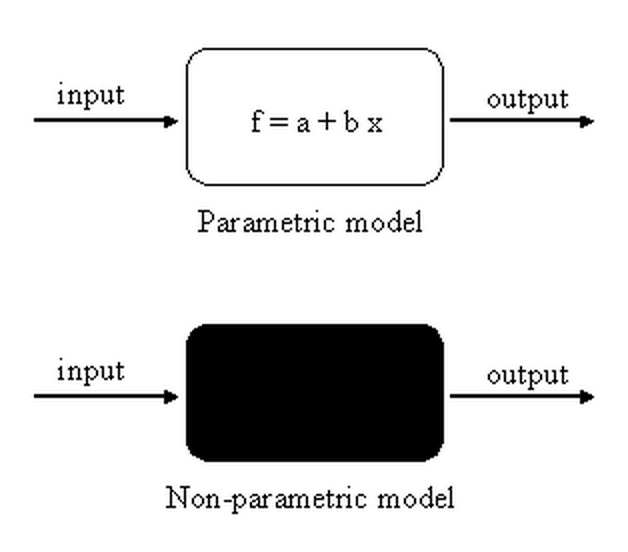
\includegraphics[width=0.3\textwidth]
    				{img/black_box.png} 
    			}}%
    			\caption{Black Box problem}%
    			\label{fig:BlackBox}
		\end{figure}	
		
		\subsubsection{The Challenges}
		There are a number of challenges that arise in attempting to change this way of working; firstly, these networks are composed of many functional components, the values of which as individuals and as a whole are not readily understood. In addition, each component of a network may have dozens of hyper-parameters linked to it, every one of which needs to be tuned to attain optimal performance. Finally, exacerbating these issues is that literature hasn't formalised methods for development or discussion, so even experts can only rely on others anecdotal results to guide network design.
		\par 
		In real terms, this means that designing and debugging deep neural networks is error-prone and time-intensive. 
		\par 
		\subsubsection{Possible Solutions}
		It is hoped that alternative work flows may provide some deeper insight. \cite{Jarrett2009} for example uses a number of pre-evaluated models compared against number of datasets to make more informed decisions, this however doesn't leave room for new discovery. \cite{Bergstra2013} uses a less human involved approach by using Bayesian statistics to automate the search of the parameter space, this is however computationally demanding and doesn't always provide an optimal solution. 
		\par 
		A further area is to support decision making with visualisation allowing for the constant evaluation of networks to help researchers better understand the trajectory they are taking their models in as they go through the standard trail and of error tweaking different parameters. This is the approach that is being explored in this project. 
		\par
\subsubsection{Existing uses of visualisation}
	It's important to stress here that this is not a novel idea, and similar projects have been undertaken across a variety of areas within Machine Learning, in the visualisations of the naive-Bayesian network \cite{Becker2001}, decision trees \cite{Ankerst1999}, Support Vector Machines \cite{Caragea2001} and Hidden Markov Models \cite{Dai2008}. Studies have shown that integrating such tools into the learning work flow can in fact produce better results than automated techniques alone \cite{Ware2002}.

\clearpage 

\section{Searching for a Solution}
	\subsection{Human \& Computer Augmentation}

\subsubsection{Solving Hard, Complex Problems in the Real World}

When former world champion chess grandmaster Garry Kasparov was beaten by IBM’s deep blue in February 1996, the headline was that Artificial Intelligence had finally surpassed human intellect. However following that loss Kasparov founded a competition known as freestyle , or advanced, chess - here human chess players use software to augment their play. The results were significant: humans who teamed up with machines could beat any of the autonomous machines. So while AI is often heralded, it's important to recognise that humans still bring important qualities to the intelligence scene. 
\\\

		$$
			\mathbb{IA} > \mathbb{AI}
		$$
	
Today far more sophisticated AI algorithms have been developed, and often included in the list of best are Deep Neural Networks. However, as mentioned earlier there is a problem - to design the networks to they perform as expected is incredibly difficult and there is a great challenge in understanding what these networks are actually doing. 

Where companies like PayPal and Palantir use machines to process data and humans to analyse it - often through visualisations - to perform complex fraud detection tasks, perhaps by using the computer as a lever to analyse large datasets (the output of neural networks) 


		\begin{figure}[H]
    			\centering	
			{{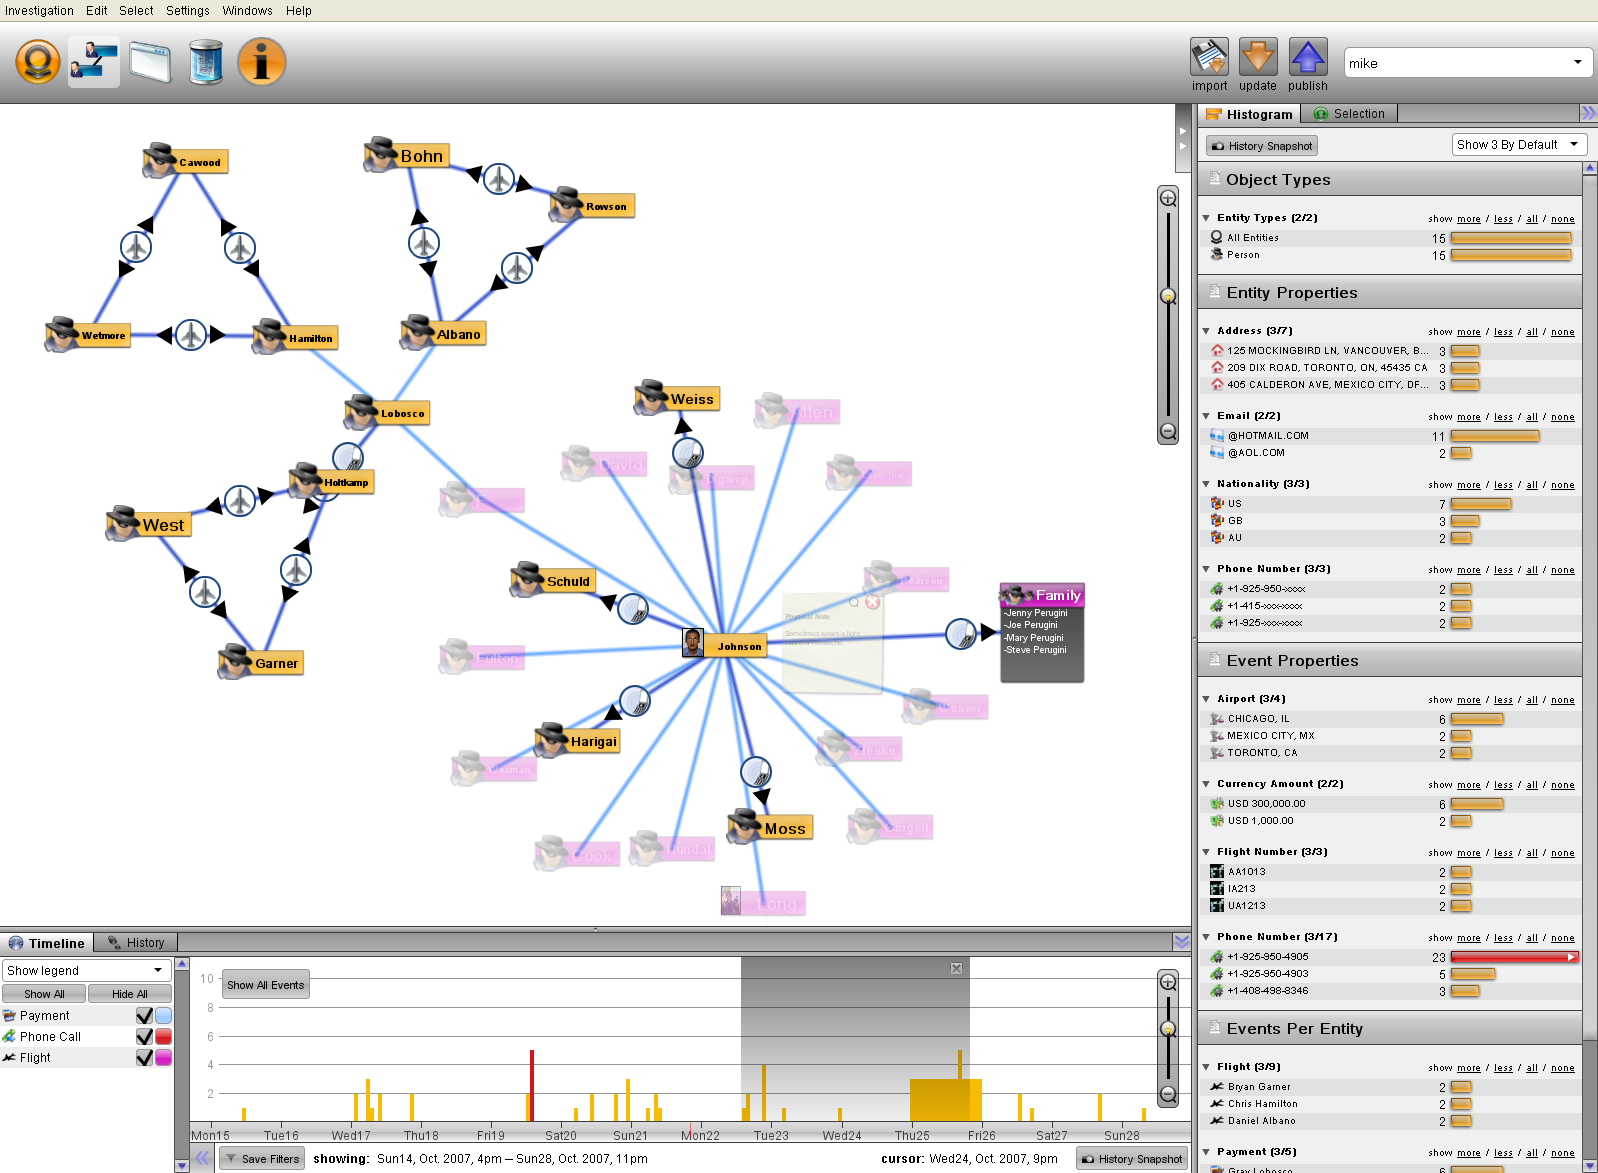
\includegraphics[width=0.4\textwidth]
    				{img/palantir_01.png} 
    			}}%
    			\caption{Palantir Screenshot Visualisation}%
    		\label{fig:Palantir}
		\end{figure}


"The use of computer-supported, interactive, visual representations of abstract data to amplify cognition" \cite{card1999}

we can develop visualisations that allow us to work with the computers data handling capabilities and human pattern recognition and understanding to understand neural networks better. 

Visualisation can help us notice things that were previously hidden. Even when data volumes are vast, patterns can be identified quickly and with relative ease. Visualisations convey information in a way that makes it simple to share ideas with others as well -  it lets people say ``Do you see what I see?” And it can even help answer questions like ``What would happen if we made an adjustment to that area?”


\subsubsection{Active Vision Problemsolving}
		
 		There has been a small revolution in our understanding of human perception, sometimes called `active vision' \cite{Ware2010}. Active vision means that we should think about graphic designs as more than pretty images, but as cognitive tools that enhance and extend our brains. Diagrams, maps, web pages, information graphics, visual instructions, and more regularly help us to solve problems through a process of visual thinking, using the enormous proportion - almost half - of the human brain that is devoted to the visual sense.  
 		
		\begin{figure}[H]
    			\centering	
			{{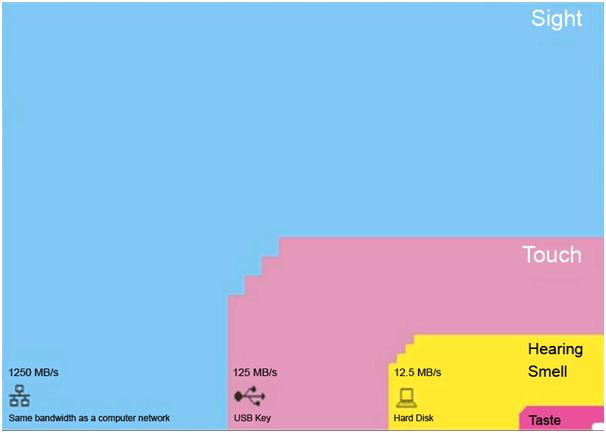
\includegraphics[width=0.3\textwidth]
    				{img/brain_bandwidth.png} 
    			}}%
    			\caption{Tor Nørretranders Brain Bandwidth}%
    		\label{fig:TufteExcellence}
		\end{figure}
		
		\par 
		Danish Physicist Tor Nørretranders discusses the ``bandwidth of our senses ” in computer terminology to give an idea of the power of this visual system. In the diagram it's important to observe the comparison to the small white box at the corner which is \textit{0.7\%} of total power and is what we are aware off when all this processing is happening \cite{Tufte2012}.		
		\\\
		\par 
		\textit{``We are all cognitive cyborgs in this Internet age in the sense that we rely heavily on cognitive tools to amplify our mental abilities. Visual thinking tools are especially important because they harness the visual pattern finding part of the brain."} \cite{Ware2010}.
		\\\
		\par 
		When producing data visualisations it is important to think about the particular details of design. What does it take to make a graphic symbol that can be found rapidly? How can something be highlighted? The problem for the designer is to ensure all visual queries can be effectively and rapidly served \cite{Keim2002}. 

	\subsection{Visualisation Theory}
	\subsubsection{Overview}
		Visualising quantitative information, such as the data produced by neural networks, typically involves displaying measured quantities, or data, by means of the combined use of points, lines, a coordinate system, numbers, symbols, words, shading, and colour. These visual forms are more rapidly understood and are easier to critique than the information underlying them \cite{DeFanti1989}, \cite{McCormick1987}, \cite{Tufte2001}.
		\par
		In a numerical format vast quantities of data can be tedious to process, and often little understanding can be gained from such complex models. Visual data on the other hand communicates to the highly developed visual pattern-recognition capabilities of humans. Indeed, a majority of our brain's activity deals with the processing and analysis of visual images. Images are pre-attentive and are processed before text in the human brain. Several empirical studies show that visual representations are superior to verbal or sequential representations across a number of different tasks; illustrate relations, identify patterns, to present overview and details, to support problem solving and to communicate different knowledge types \cite{Burkhard2004}. As a species we are far better at recognising regularities, anomalies, and trends in images rather than in long lists of numbers \cite{Ware2010}. Consider how difficult is may be to observe both global and local patterns in a list of numbers, in comparison to the relative ease when presented in a standard visualisation model such as a graph.
		\par 
		For data mining to be effective, it is important to include the human in the data exploration process and combine the flexibility, creativity and general knowledge of the human with the enormous storage capacity and computation power of computers. Visual data mining techniques have proven to be of high value in exploratory data analysis and they have high potential for exploring large datasets.
			  		 
  		\begin{figure}[H]
    			\centering	
			{{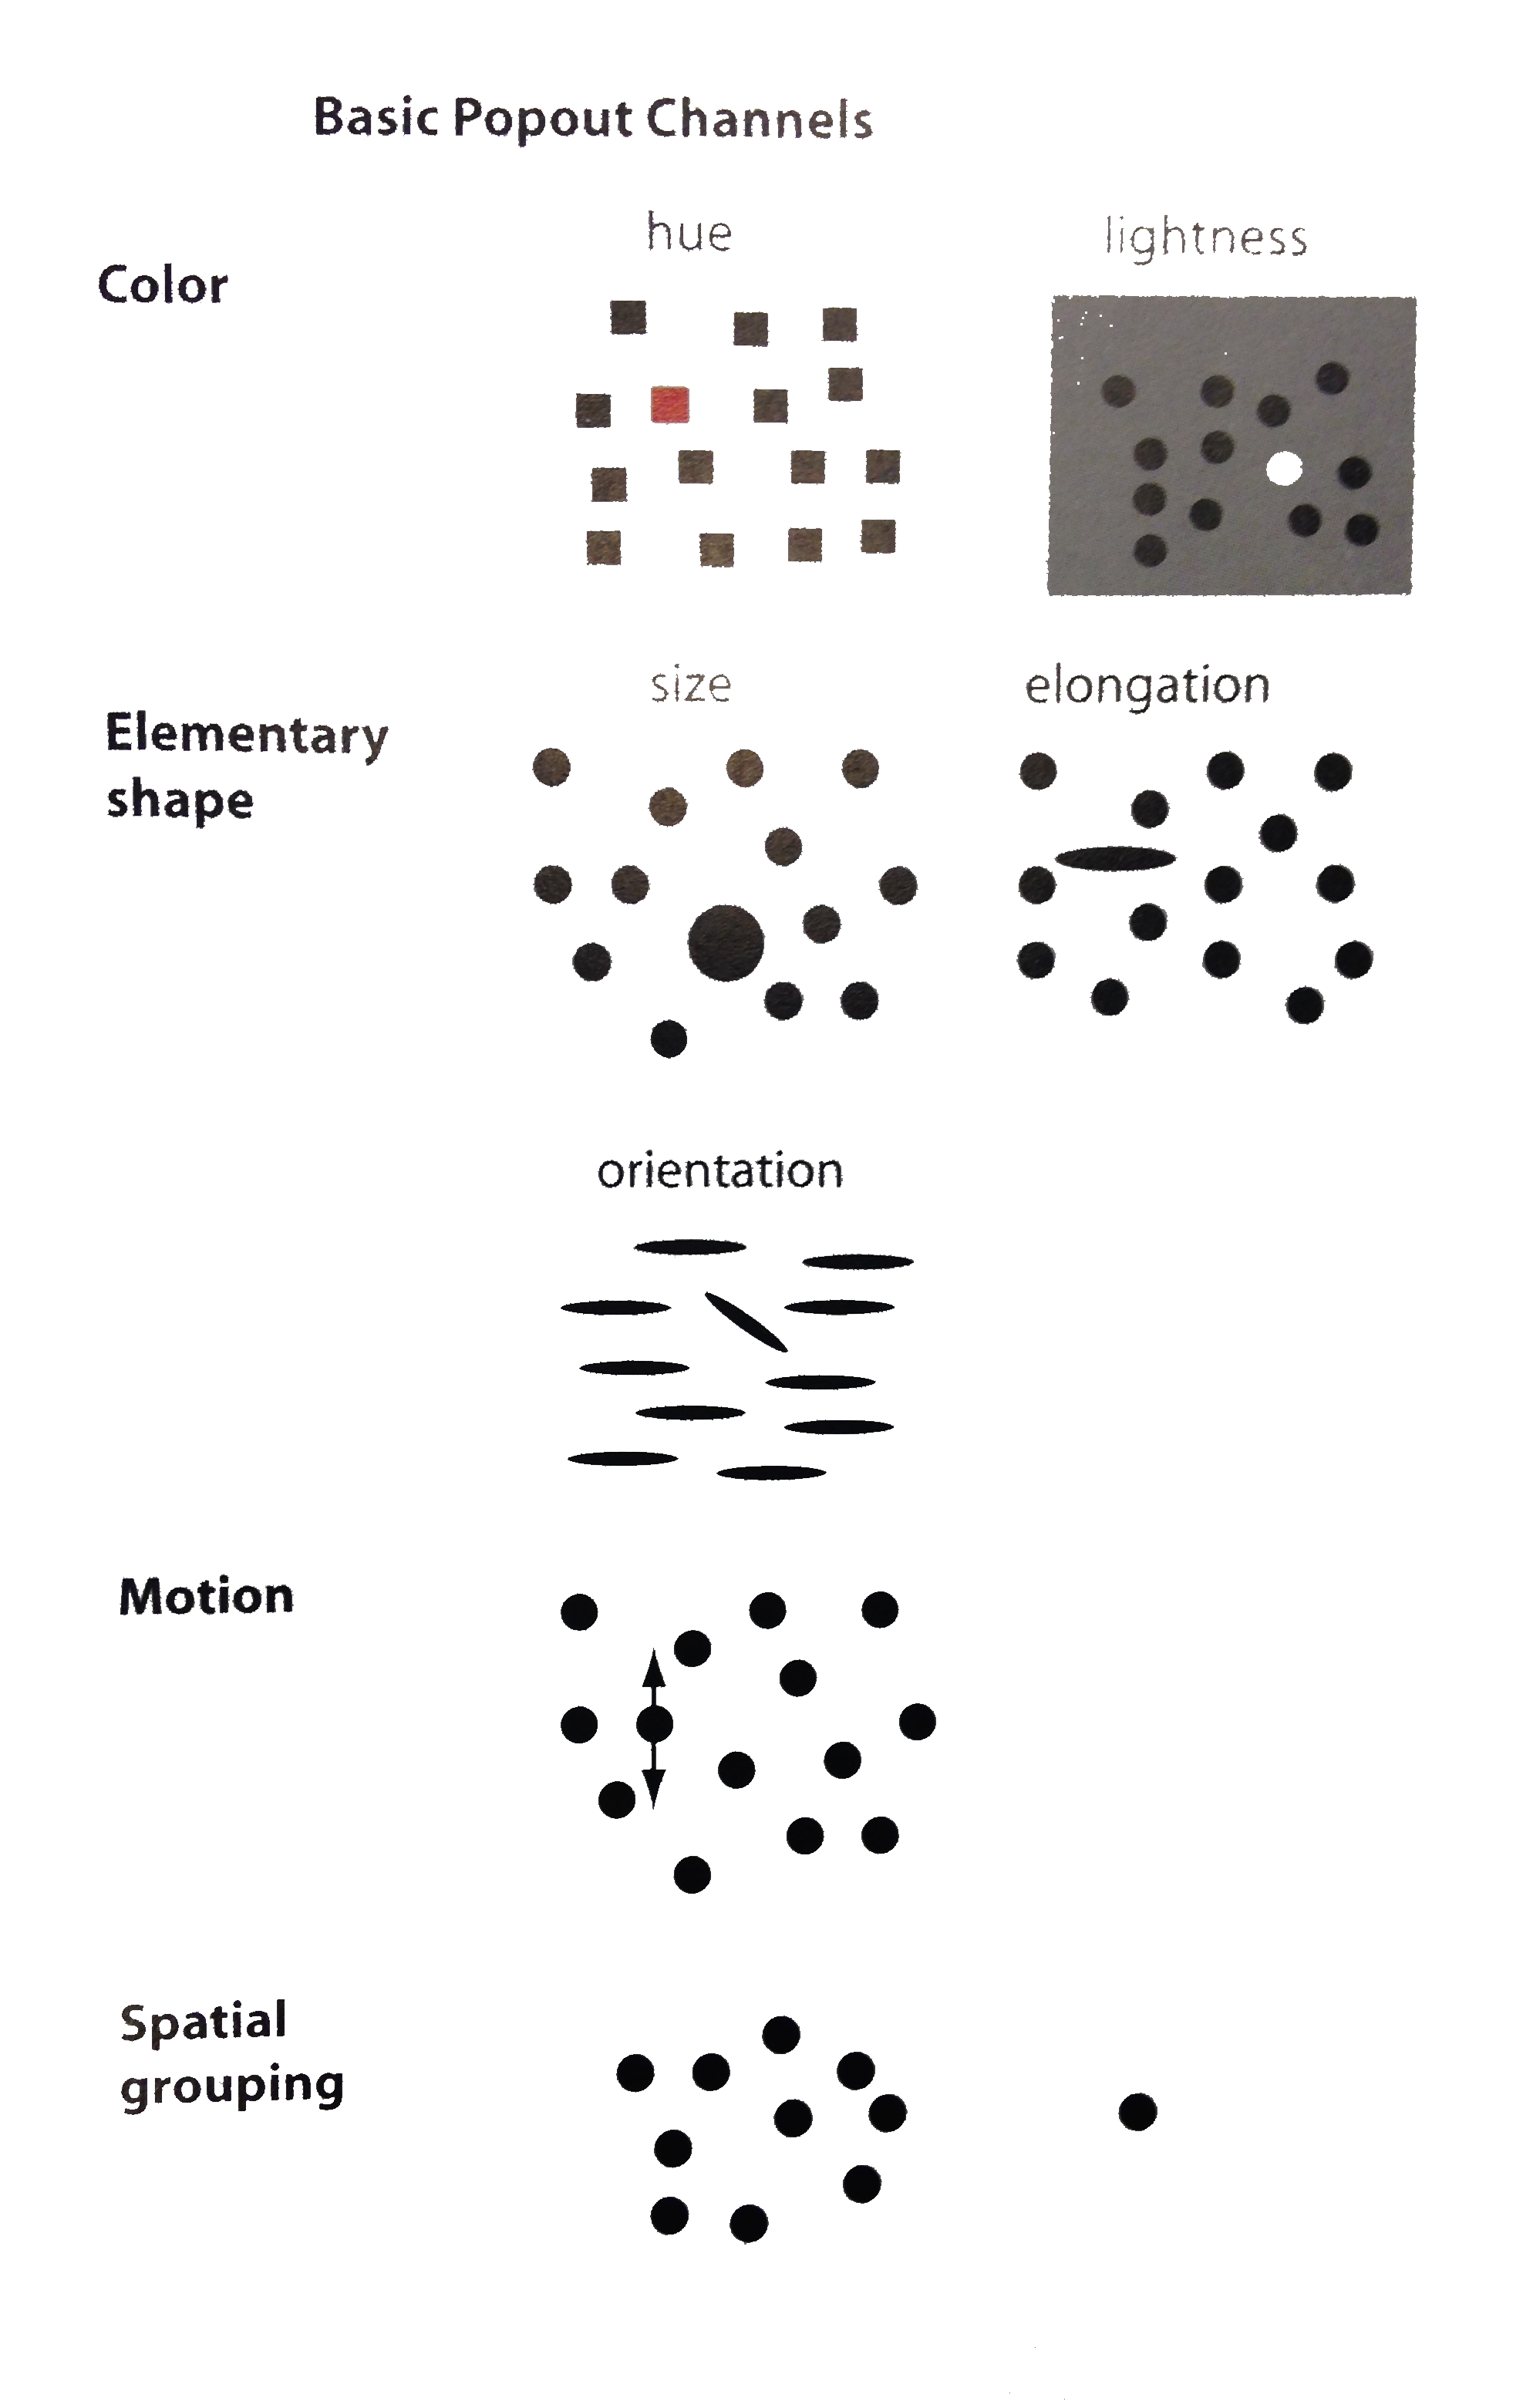
\includegraphics[width=0.4\textwidth]
    				{img/ware_popout_channels.png} 
    			}}%
    			\caption{Ware's ``Things that pop-out"}%
    		\label{fig:Ware Pop-Out}
		\end{figure}
		
		\par 
		Visual data exploration is especially useful when little is known about the data and the exploration goals are vague - such as when attempting to understand the inner workings of a neural net. Since the user is directly involved in looking at the visualisation, shifting and adjusting the exploration goals of the human eye can be automatically \cite{Keim2002}.
		\par 
		The canonical example of the usefulness of visualisation lies in the Anscombes quartet, where the four sets of numbers in the quartet have many identical summary statistics - mean of x values, mean of y values, variances, correlations and regression lines - but vary wildly when graphed \cite{Shoresh2011}:

		\begin{figure}[H]
    			\centering	
				{{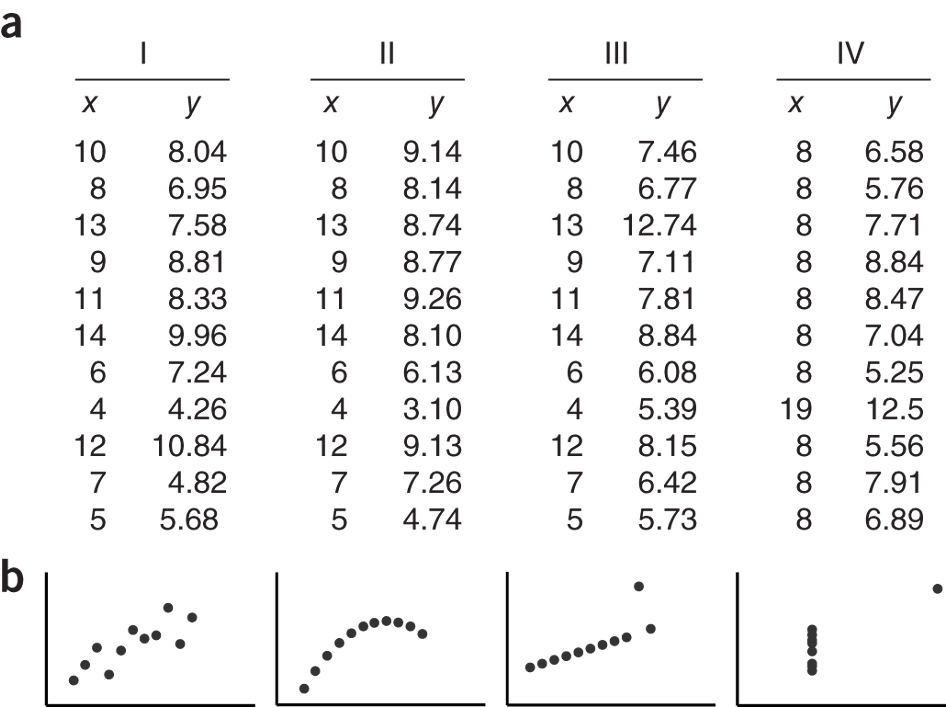
\includegraphics[width=0.5\textwidth]
    				{img/anscombes_quartet} 
    			}}%
    			\caption{(a) The four sets of numbers that form Anscombe's quartet -  (b) The highly distinctive graphs that result from plotting the data in a.}%
		\end{figure}


%\subsubsection{Tufte: what makes a good visualisation}

\subsubsection{Tufte's Rules}
		\par 
		Edward Tufte, a founding figure in laying out the core principles of data visualisation, provides us with a set of basic commandments \cite{Tufte2001}:		

		\begin{figure}[H]
    			\centering	
    			\subfloat[Poor Line Weights: unclear]												{{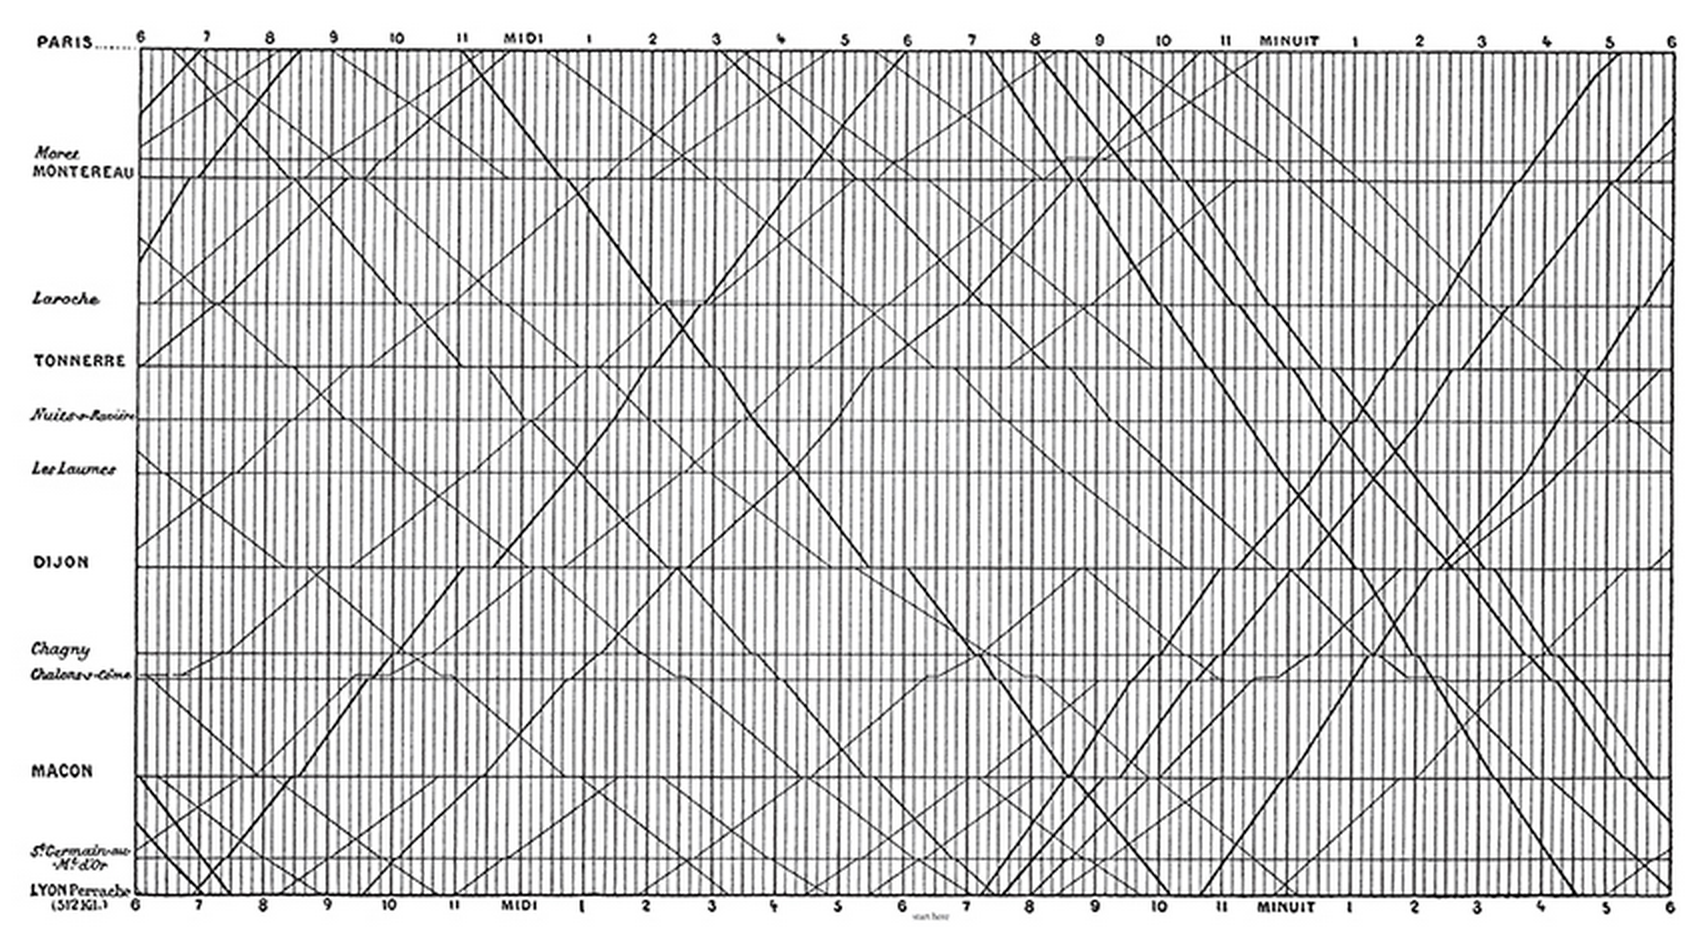
\includegraphics[width=7cm]
    				{img/marey_train_bad.png} 
    			}}%
    			\qquad
    			\subfloat[Better Line Weights: clear]
    			{{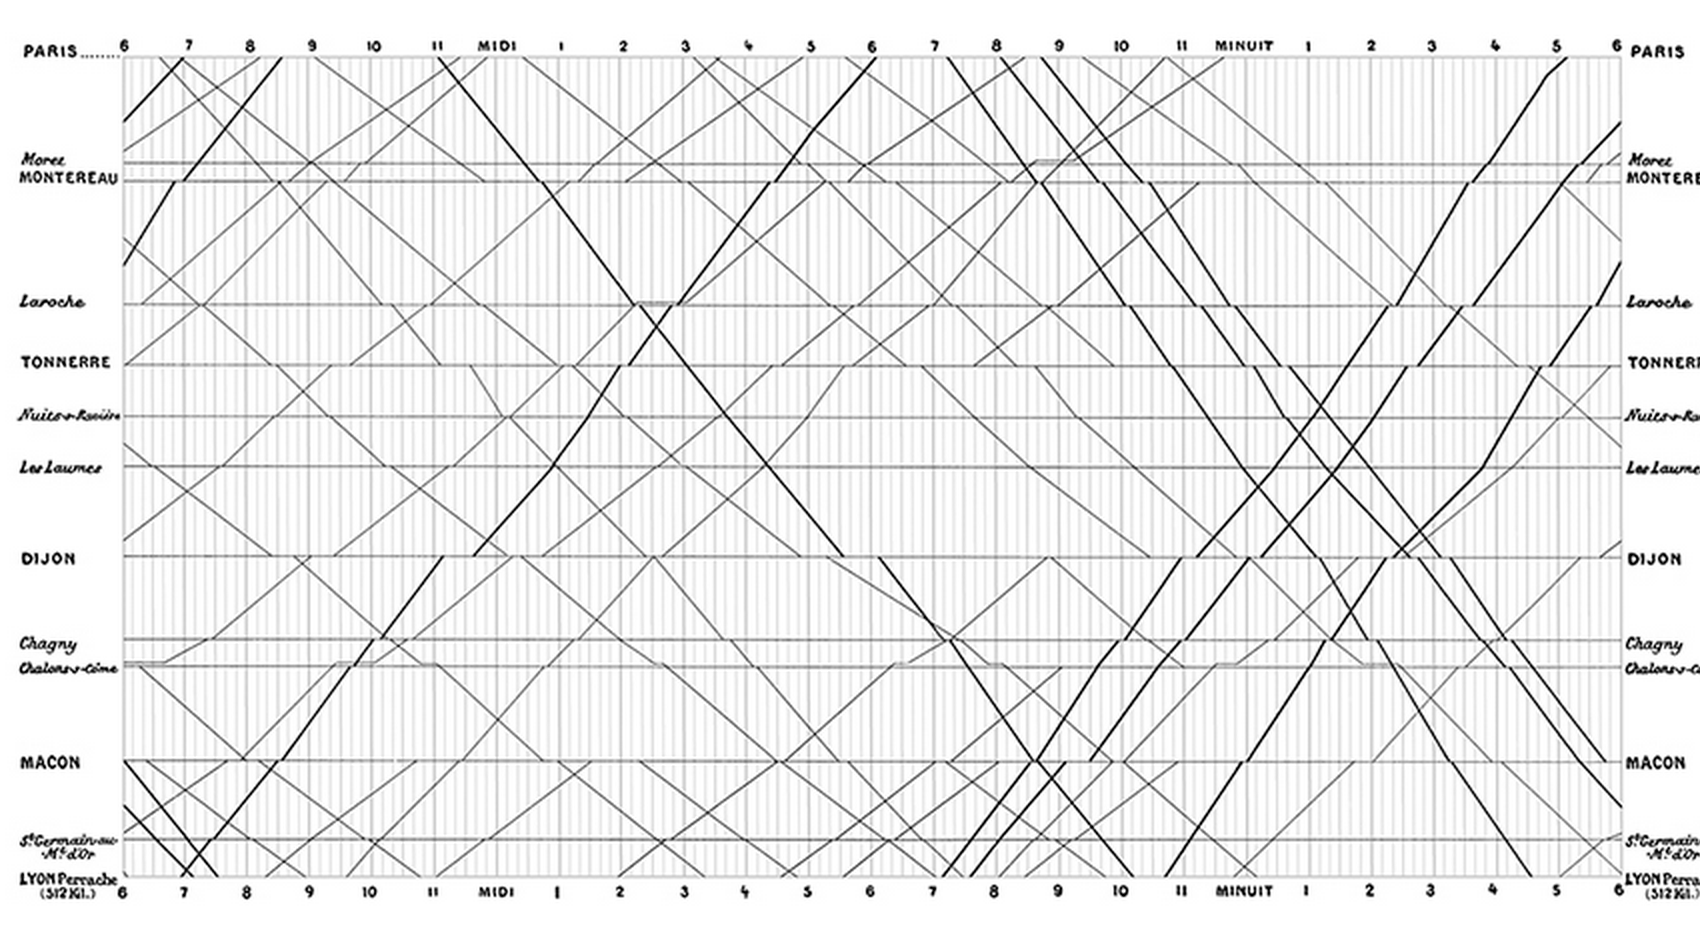
\includegraphics[width=7cm]
    				{img/marey_train_better.png} 
    			}}%
    			\caption{Tufte's train line chart demonstrating excessive data-ink}%
		\end{figure}

		\par
	\begin{itemize}
		\item \textbf{Principle One:}
		\textit{show only as much information as is required}
		\par 
		This is Tufte's \textit{data-ink} principle - irrelevant content is distracting, so should be removed. It is common place today to find charts and graphs with all sorts of three dimensional effects, unwanted background images and colours. The idea of having a data-ink ratio is to show only as much information as is required.
		$$
		\text{Data-ink ratio} = 
		\frac{\text{data-ink}}{\text{total ink used to print the graphic}}
		$$

		\item \textbf{Principle two:}
		\textit{include visual differences only when required} 
		\par
		The human brain has an amazing capability of spotting visual differences such as color, size and position. Often they look for the meaning to change depending on how these visual features and designed. If there is no difference, but embellishments are added, it often leads to confusion.

		\item \textbf{Principle tree:}
		\textit{use visual encodings for quantitative values}
		\par 
		Successful examples are: length, for example the length of bar in a bar graph; 2-D location, for example the position of a data point in a scatter plot; size, for example the area in a pie chart; shape, orientation or hue, for example denoting different classes in any graph. All of these are automatically and immediate understood as they have natural properties that humans understand. 

		\item \textbf{Principle four:}
		\textit{differences in visual properties should correspond to actual differences in the data}
		\par 
		Its important to encode differences consistently and not manipulate the visualisation to aid an argument. For example, ensuring that axes are consistent - from zero to some useful value without undergoing any form of distortion.

		\item \textbf{Principle five:}
		\textit{do not visually connect values that are discrete}
		\par 
		In a graph, when you draw lines between discrete values and connect them, people perceive those values as having a relationship to each other, and so this should be avoided.

		\item \textbf{Principle six:} \textit{visually highlight the most important part of your message}
		\par 
		All information on a chart might not be equal and it might be possible to direct a users attention to a particular part of the visualization by visually highlighting through use of color, position or another standard encoding.

		\item \textbf{Principle seven:} 
		\textit{augment short term memory through visual patterns}
		\par
		The human brain is limited to retaining around four pieces of information at any given time. By presenting quantitative information as visual patterns, more information can be simultaneously stored as one `piece'.
	\item \textbf{Principle eight:}
	\textit{Encourage the eye to compare different pieces of data}
	\par
	Information is not something that exists in isolation, and often by comparing pieces of information one is brought to new conclusions about that data.
	\item \textbf{Principle nine:}
	\textit{Reveal the data at several levels of detail}
	\par
	Quantitative data often has several scales, with patterns appearing at both a global and local level. By enabling the data to be viewed at different levels of detail the data can be explored in all it's complexity.
	\item \textbf{Principle ten:}
	\textit{Don't distort the data:}
	\par
	Often it is tempting to change the scale on a graph for it to 'fit' appropriately, or to crop the data hiding anomalies. With these elements of distortion the full picture is not revealed, and the purpose of visualisation compromised. 
	\end{itemize}
\subsection{Existing NN Visualisations}
		
	 Visualisation has been around helping researchers with neural networks for a long time, and techniques such as the \textit{Hinton diagram} were first demonstrated as early as 1986. This section provides a brief overview of similar techniques from around the nineties, where a number of the techniques are going to be visualisations of fig. \ref{simplenet}.
	 
	 	\begin{figure}[H]
    			\centering	
			{{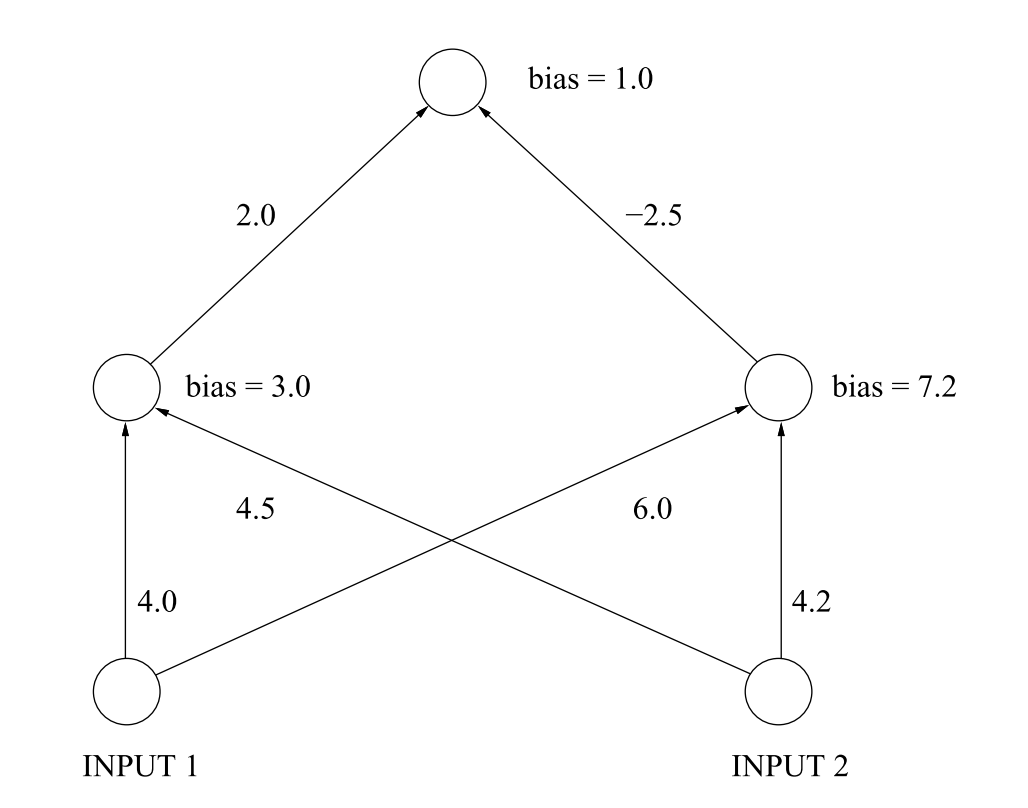
\includegraphics[width=0.3\textwidth]
    				{img/craven_simple_net.png} 
    			}}%
    			\caption{Simple Neural Network}%
    		\label{fig:simplenet}
	\end{figure} 	
		
%\subsubsection{Hinton Diagram}
\subsubsection{Hinton Diagram}

		 		
 	\begin{figure}[H]
    			\centering	
			{{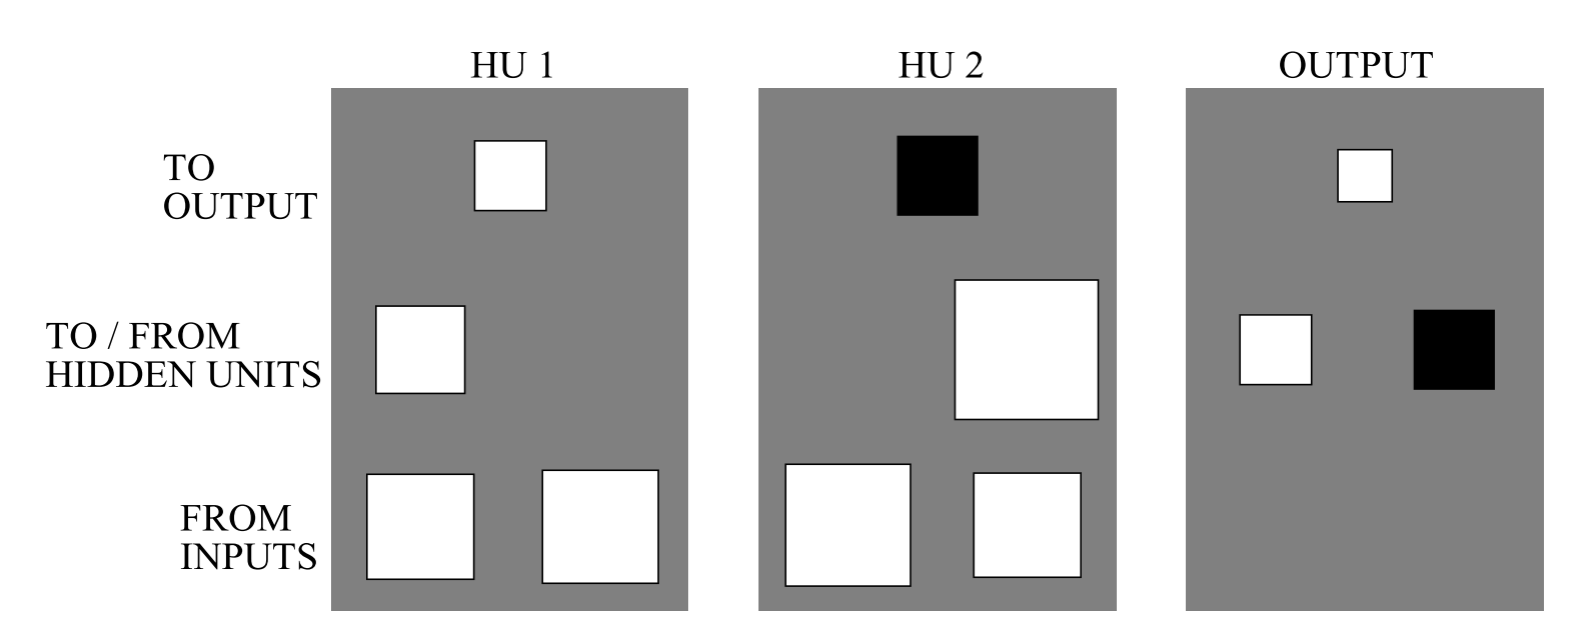
\includegraphics[width=0.3\textwidth]
    				{img/craven_hinton.png} 
    			}}%
    			\caption{Hinton Diagram}%
    		\label{fig:simple}
	\end{figure} 
 		
		One of the first practical visualisations of ANNs was the \textit{Hinton Diagram} \cite{Hinton1986}. It visualises the weights and biases related to a node within a network. Weights are represented as boxes, where its area represents the weights magnitude, and it's shade represents the sign on the weight - white is positive, black is negative. Biases are illustrated as weights from a node back to itself. There is a vague representation of the architecture as output nodes appear at the top of a diagram, hidden nodes are in the middle, and input nodes are at the bottom. However these diagrams are rather unclear, and lack of topological information is a problem. The advantage is they make it easy to see the signs and magnitudes of the weights that contribute to a neurons activation.
		\\\
		\\\
		
%\subsubsection{Bond Diagram} 
\subsubsection{Bond Diagram}		
 	\begin{figure}[H]
    			\centering	
			{{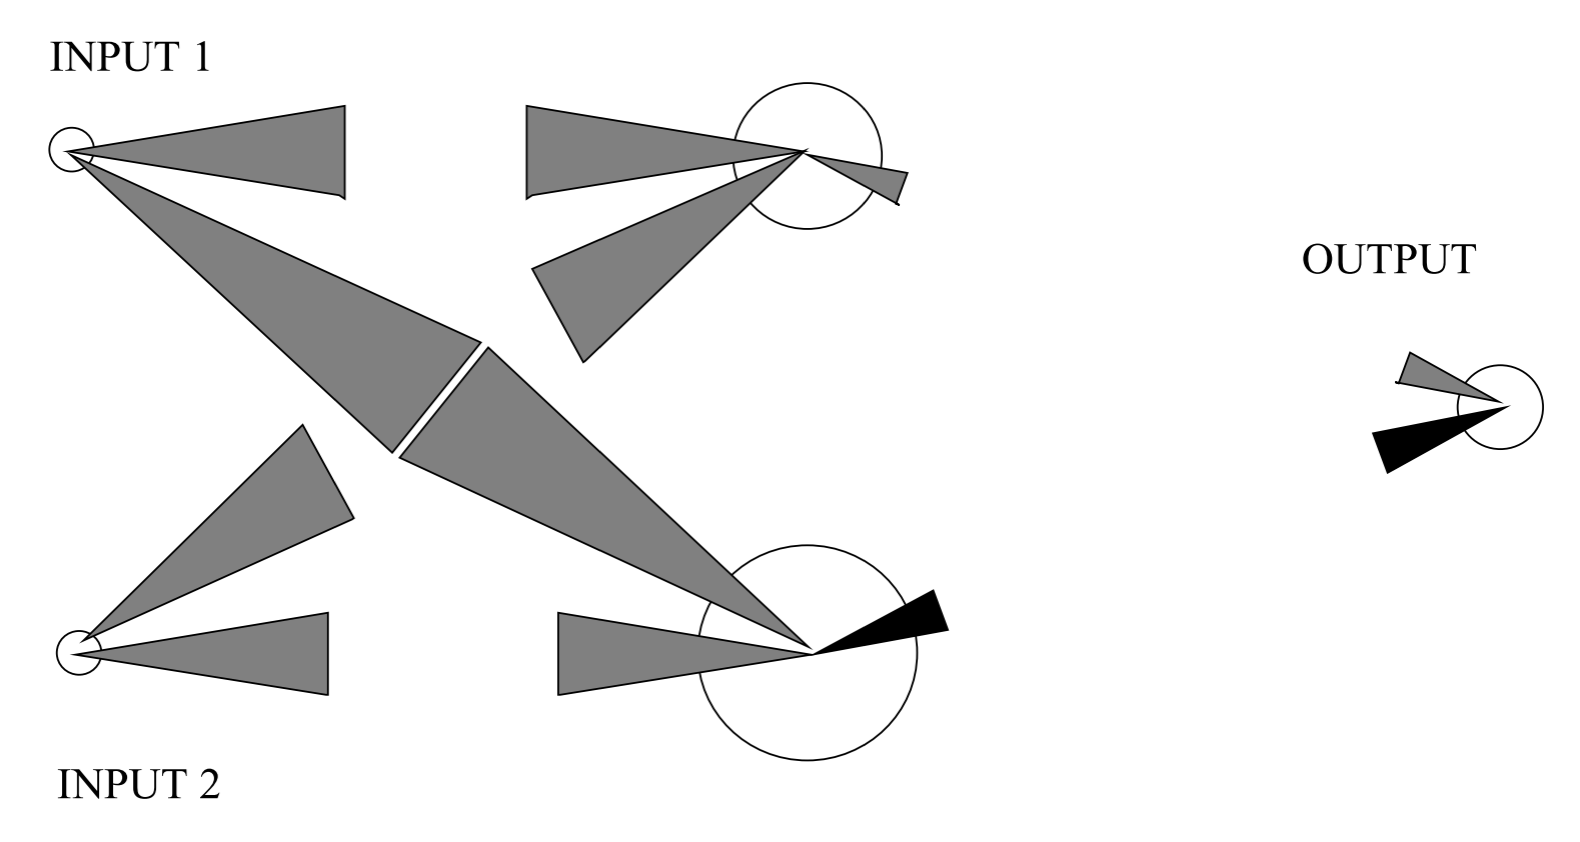
\includegraphics[width=0.3\textwidth]
    				{img/craven_bond.png} 
    			}}%
    			\caption{Bond Diagram}%
    		\label{fig:bond}
	\end{figure} 
 		
		Similar to the \textit{Hinton Diagrams}, the Bond diagram \cite{Wejchert1990} graphically depicts the values of the networks weights and biases. The bond diagram however attempts to make the architecture of the network more clear; a neuron is depicted as a circle, where the diameter of the circle indicates the magnitude of the bias, and triangles connecting the circles represent the weights. The magnitude is indicated by the height of the triangle, and colour depicts the sign. 
		\par 
		While it is perhaps easier to decipher the network structure from the Bond diagram, it is harder to gauge the relative importance of the weights and biases which have been depicted with different shapes. It makes the following question very difficult to answer: ``which input units need to be active in order for the net input to exceed the threshold (bias) of the hidden units?" \cite{Craven1992}, a useful question that Hinton diagrams are far better at answering.
		\par 
		
\subsubsection{Hyperplane Diagrams}
%\textbf{Hyperplane Diagrams}
		
 	\begin{figure}[H]
    			\centering	
			{{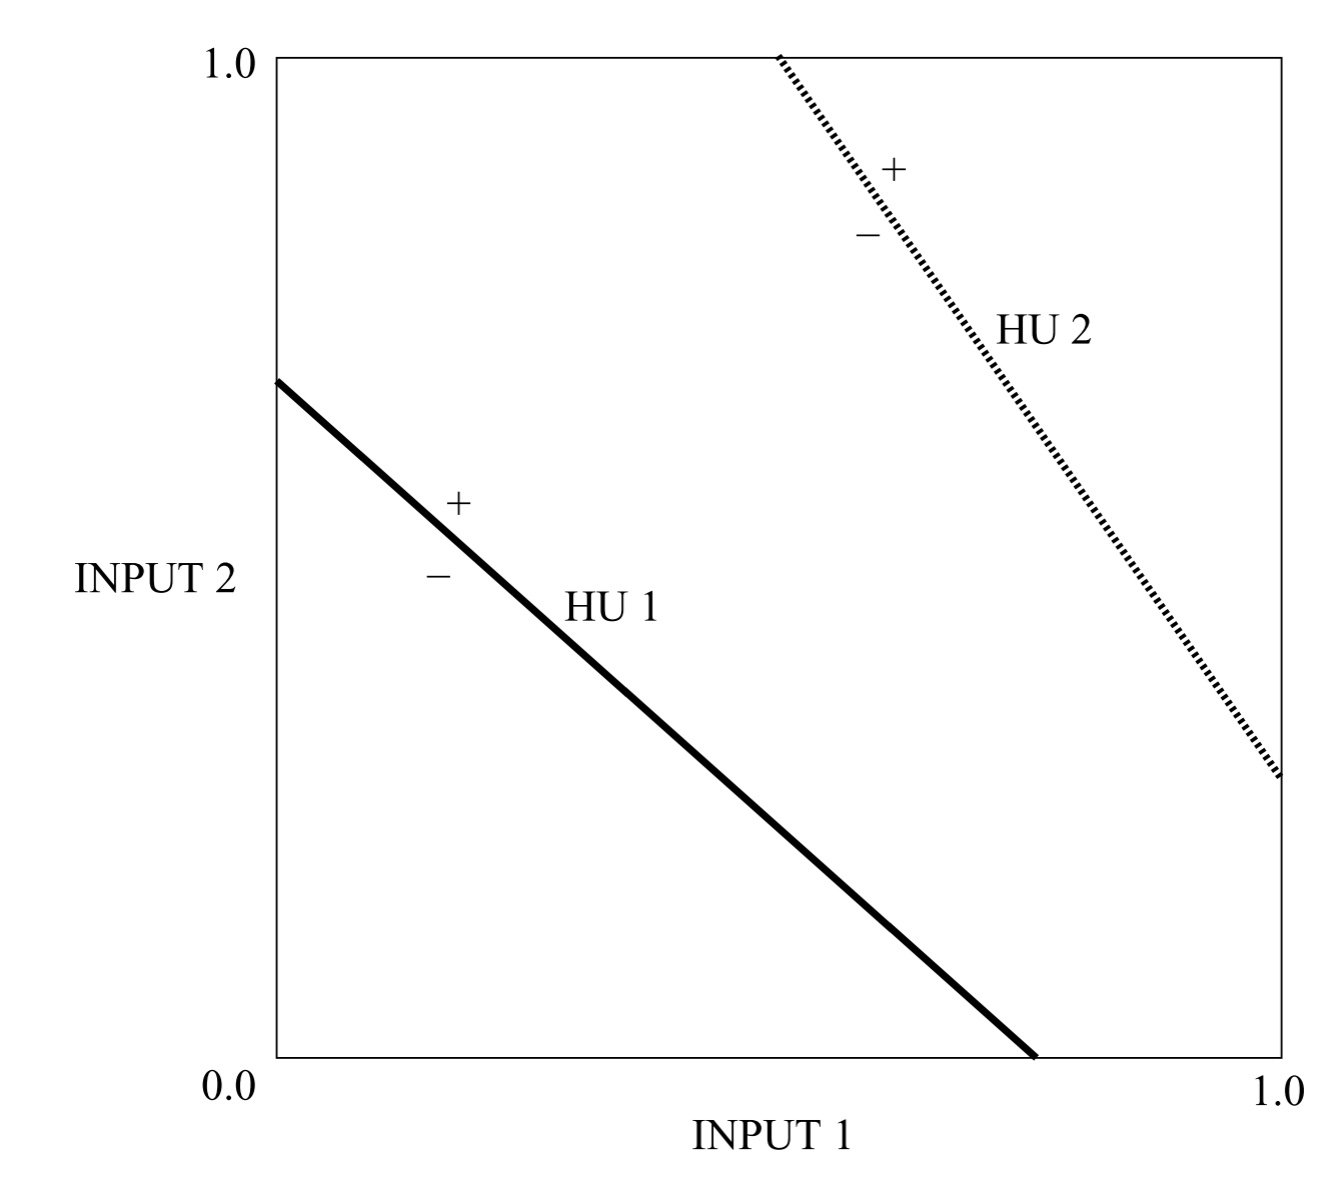
\includegraphics[width=0.3\textwidth]
    				{img/craven_hyperplane.png} 
    			}}%
    			\caption{Hyperplane Diagram}%
    		\label{fig:bond}
	\end{figure} 
 		
		A hyperplane depicts the `threshold' of a decision surface. As this hyperplane moves throughout the training process, visualising the hyperplane as it moves can be a useful method to get an understanding of what a neuron is learning \cite{Munro1992}. Neurons that appear in the same layer can have their hyperplanes shown in the same diagram due to a sharing of input space, making comparison easy.
		\par 
		One issue with this hyperplane representation is that while accurately representing a threshold function acting on a two-dimensional input space, the diagrams fall down when compared with most contemporary ANNs that require multiple dimensions (>3) to be shown and more commonly use continuous transfer functions such as  the sigmoid - which requires a gradual, rather than a sudden, division of the input space. That said, it can be assumed that the hyperplane is a close approximation of the gradual boundary and so can still provide useful observations.
		\par 
		
\subsubsection{Response-function plots}
%\textbf{Response-function plots}
		
 	\begin{figure}[H]
    			\centering	
			{{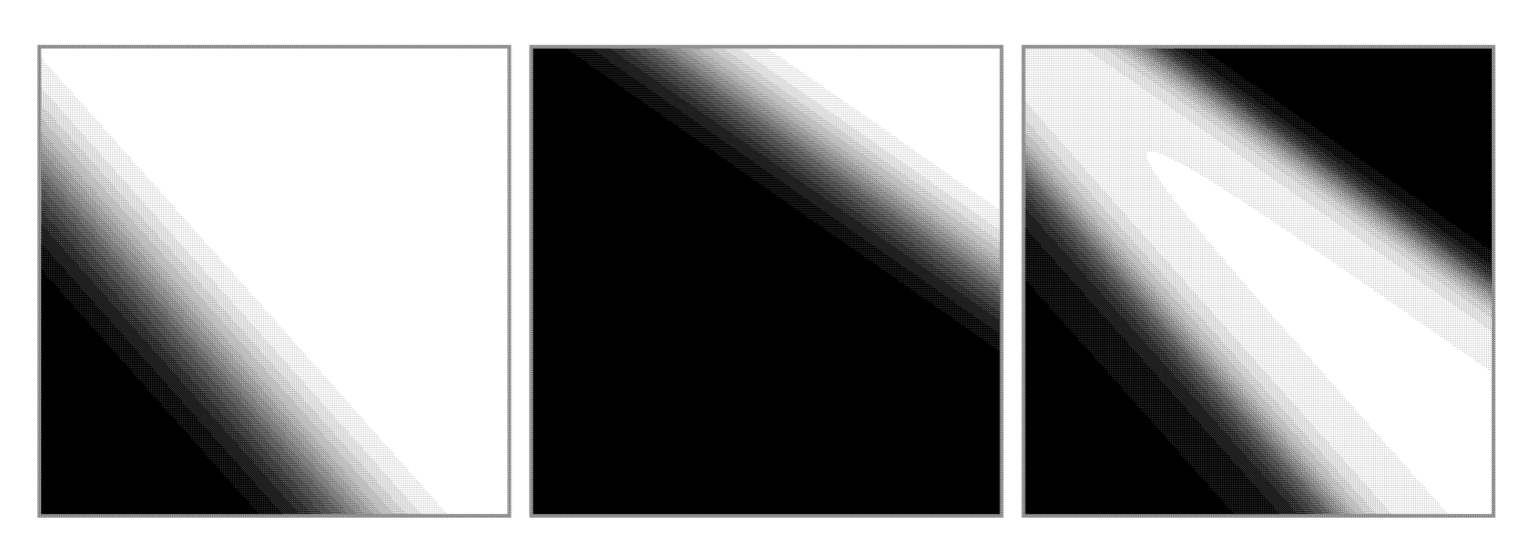
\includegraphics[width=0.3\textwidth]
    				{img/craven_gradient.png} 
    			}}%
    			\caption{Response Function Plot}%
    		\label{fig:bond}
	\end{figure} 
 		
		Response-function plots are very similar to hyperplane diagrams - they also display the decision surface. They differ in their solving of the issue of the gradual boundary. Instead of displaying the space using a hyperplane, the space is displayed as a gradient of values to indicate the resulting activations.
		\par 
		Interestingly, both the Response-Function Plots and the hyperplane diagrams show the space between two successive layers of neurons. This provides only a fraction of information about the network, and problematically may lead to false assumptions about it. One way to address this is to describe the decision surface not just on the layer below, but across all previous layers of the input space.
		\par 
		
\subsubsection{Trajectory Diagrams}
%\textbf{Trajectory Diagrams}
		
 	\begin{figure}[H]
    			\centering	
			{{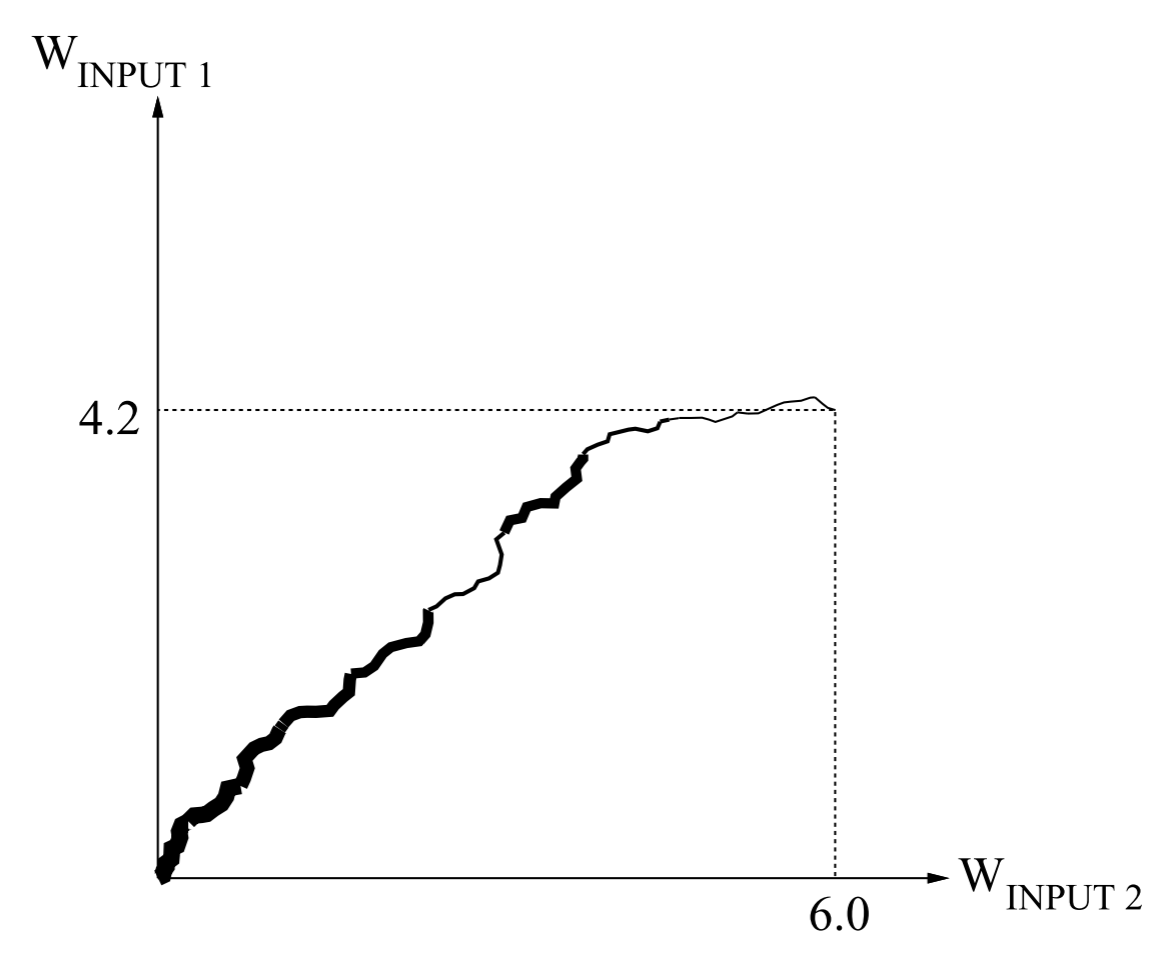
\includegraphics[width=0.3\textwidth]
    				{img/craven_trajectory.png} 
    			}}%
    			\caption{Trajectory Diagram}%
    		\label{fig:bond}
	\end{figure} 
 		
		Trajectory Diagrams \cite{Wejchert1990} depict the change in weight space and in error over a neuron during training. These diagrams use the incoming weights of a neuron to create the axes of a plot. During training as the weights change they are visualised as a trajectory in the weight space. The error at a given time is indicated by the thickness of the trajectory line.
		\par 	
		Again, along with many of these other early visualisation methods, the weakness of the trajectory diagram is its inability to display weight spaces of more than three dimensions. There have been efforts to combine dimensionality visualisation with trajectory diagrams - such as using radially projected axes, however this is fairly unsuccessful \cite{Craven1992}. 
		\par 
		
\subsubsection{Lascaux}
%\textbf{Lascaux}
		
	\begin{figure}[H]
    			\centering	
			{{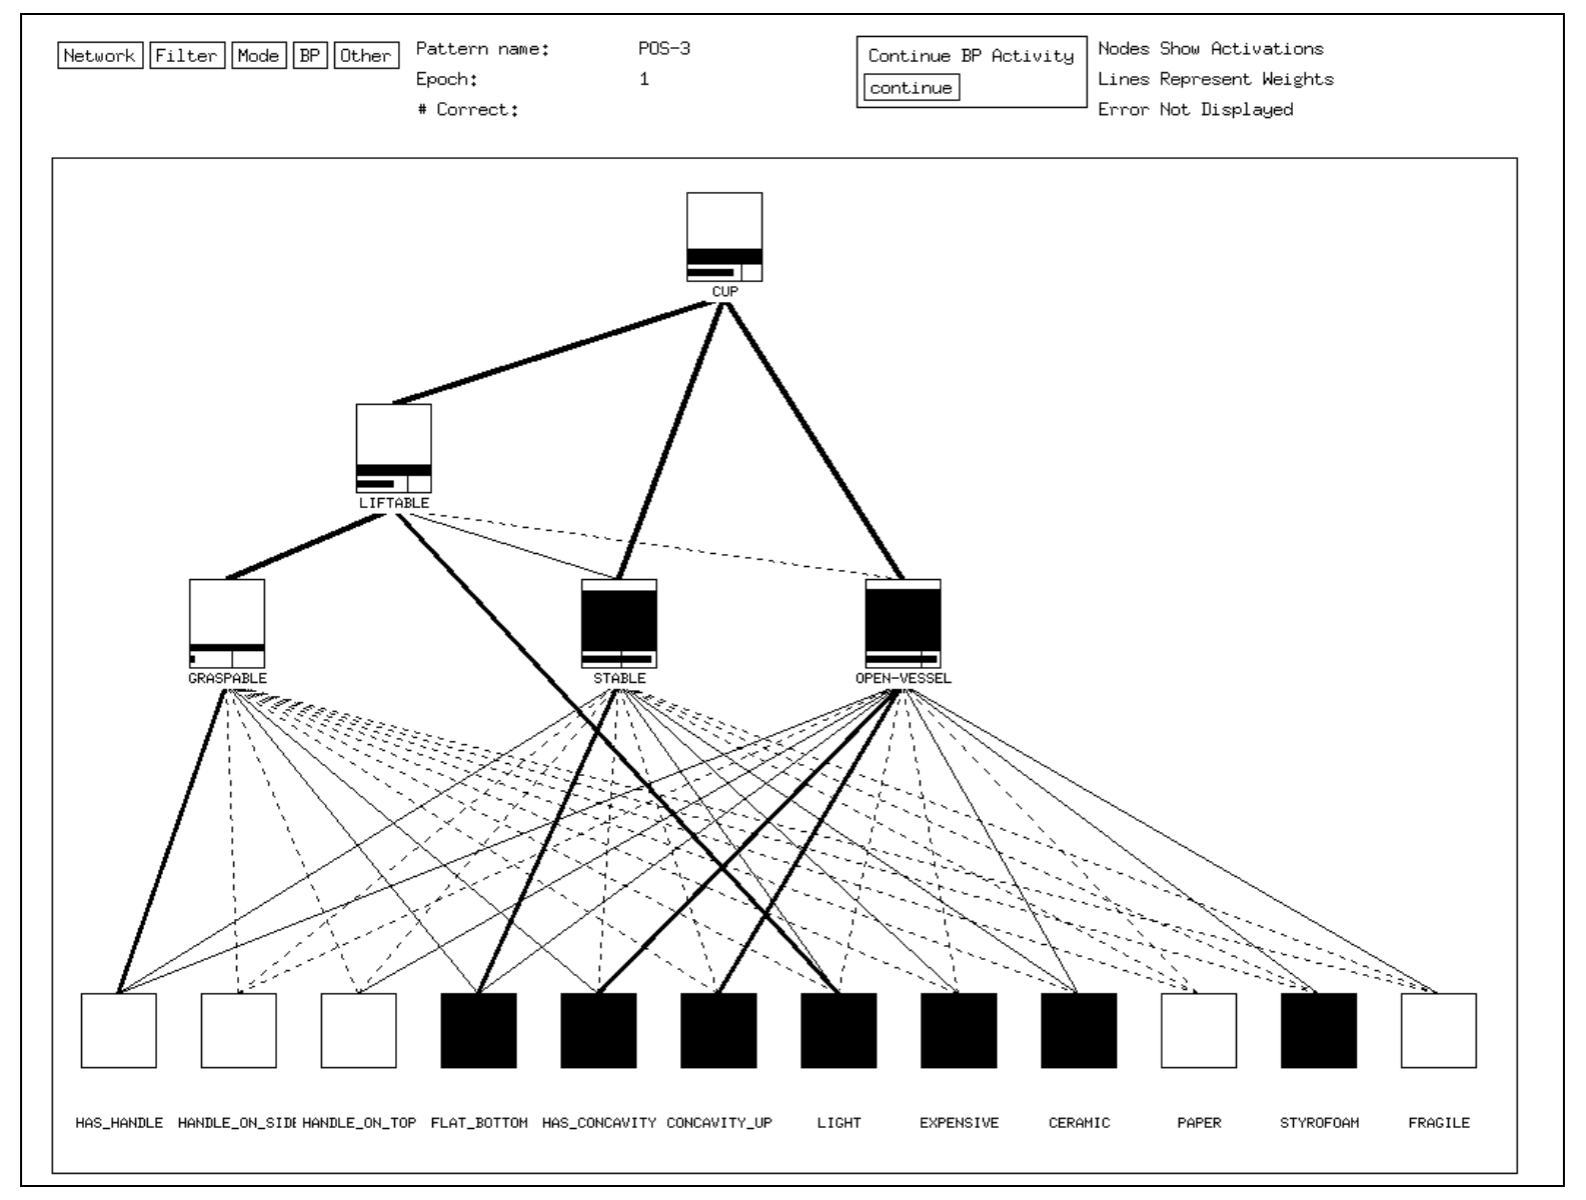
\includegraphics[width=0.3\textwidth]
    				{img/craven_weights.png} 
    			}}%
    			\caption{Lascaux Clip}%
    		\label{fig:lascaux}
	\end{figure}  		
 		
		Lascaux is a visualisation tool proposed by \cite{Craven1992} that aimed to clearly display the topology of a network. Here, each neuron is represented as a box and network weights are represented by interconnecting lines. A weights magnitude is visualised by the thickness of a line, and the positive or negative signs are visualised as solid and dashed lines respectively.
		\par 
		The tool depicts a range of information it one place. Activation of each neuron is show as a vertical bar within the neuron `box'; a horizontal bar shows the net input relative to a threshold - shown as a line intersecting the bar; error is another vertical bar within the neuron box; a separate diagram shows the error propagating as connections between these boxes - where thickness describes magnitude.
		\par 
		The issue with \textit{Lascaux} is that too much information is being displayed in a small space ineffectively. The approach uses standard two dimensional visualisation techniques, and simply squashes them into a neural network architecture. This makes the topology easier to understand, but at the sacrifice of more important elements.

\subsubsection{Visualising Weights and Connections}
%\textbf{Visualising Weights and Connections}
		When representing weights, it is important to consider the analytical impact of a visual decision. \cite{Streeter2001} visualises the topology of the network but doesn't clearly show the weights themselves. This can lead to confusion when assessing the importance of a neuron. Consider for example a neuron that has appears to have a high value in one layer, however is subsequently cancelled out by low weights deeper within the network.
	\par 
	One problem here is that since the absolute values of the weights are used, the result does not provide the direction of the relationship. 
	\par 
		
	\begin{figure}[H]
		\centering 
    		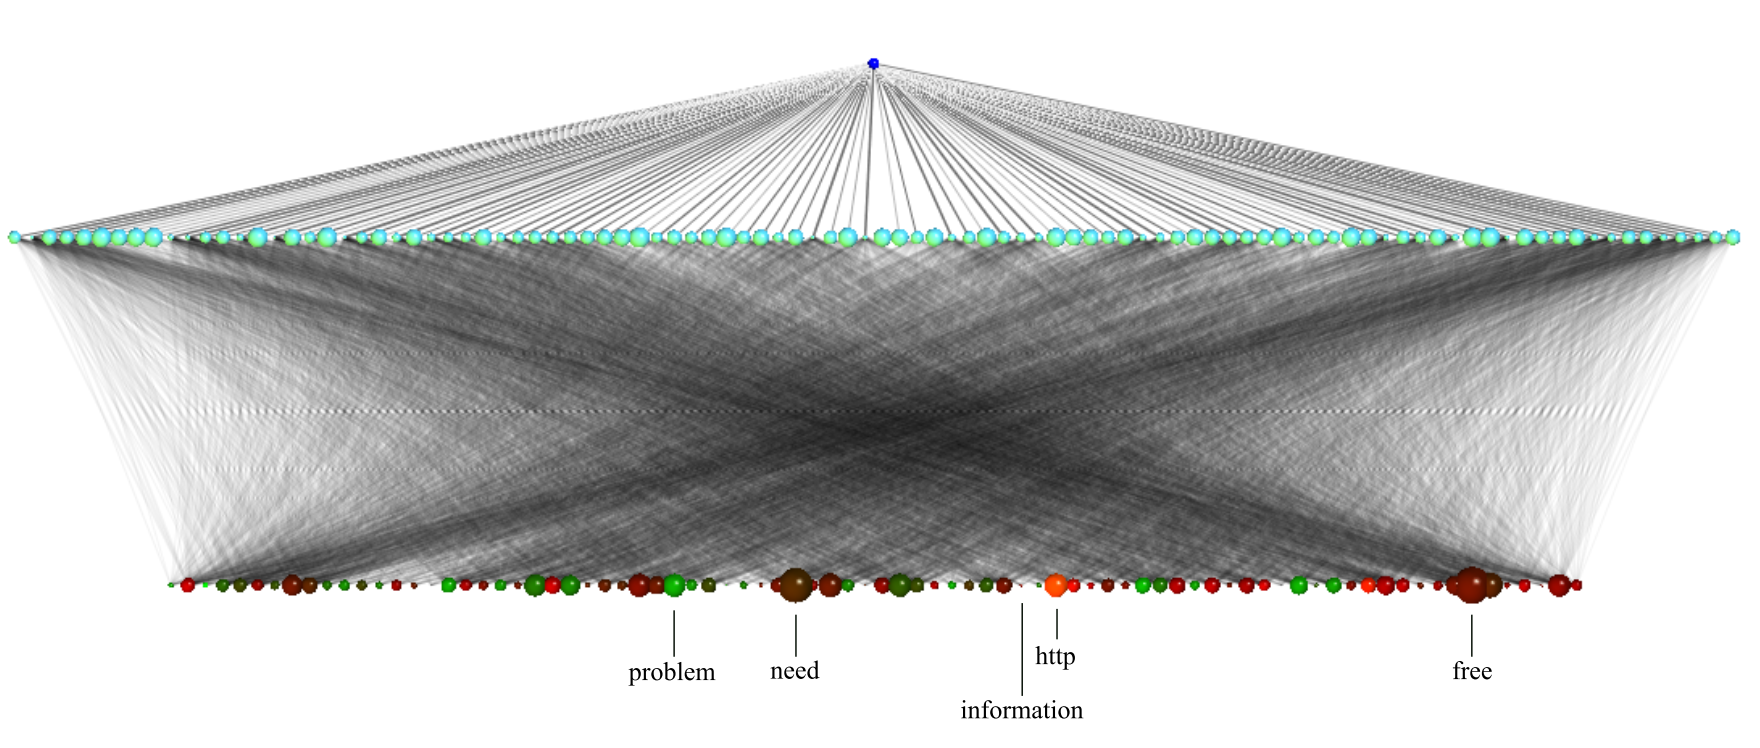
\includegraphics[width=0.7\textwidth]{img/tzeng_large_map.png} 
    		\caption{Tzeng Map}%
 	\end{figure}
 	
	\cite{Tzeng2005} based on the work of 	\cite{Garson1991} and \cite{Goh1995} sought to solve this problem in a different way; by visualising the weights with line-thickness between nodes, thus making it easy to identify when a node is insignificant regardless of the magnitude of weights applied to it.
	\par 
	In addition 	\cite{Tzeng2005} propagate all of the layers influence through the network by multiplying each weight between the previous layers with those of the successive layers which connect to the same node. Here, they represent the contribution of a specific hidden node by adjusting the diameter of the circle visualising the neuron in their visualisation. The contribution of the input unit $ i $ to the output unit $ o $ through a hidden unit $ j $ is computed by multiplying the input-hidden weight strength and the hidden-output weight strength:
$ r_{ijo} = w_{ij} \times w_{jo} $, and the relative contribution from each input node $ k $ to a hidden node $ j $ can be represented as:
		$$
		r_{ijo} = 
		\text{ $ \frac{|C_{ijo}|}{\sum\limits_{k=1}^m |C_{kjo}| } $ }
		$$ 
	where the total contribution from an input node $ i $ is: 
		$$
		S_{i} = 
		\text{ $ \sum\limits_{j=1}^n r_{ijo} $ }
		$$ 
	and the relative importance of an input node is therefore:
		$$
		RI_{i} = 
		\text{ $ \frac{S_{i}}{\sum\limits_{k=1}^m S_{k} } $ }
		$$ 
	 \par 
 		
	 This combination of statistical analysis and weight representation allows for a visualisation that demonstrates not only the raw data, but an abstraction that is more useful to the researcher given the relative importance of the nodes, and significance of the data - while still providing an architectural understanding of the network. This combination of mathematics and visualisation is one that continues across a number of other visualisation techniques for neural networks.
	 
\subsubsection{Features}
%\textbf{Features}

		Another popular part of visualising neural nets, is visualising the features of a CNN to gain an intuitive understanding about its internal behaviour is becoming commonplace, it is mostly limited to the simple visualisation of the 1st layer where projections to the pixel space are relatively easy to achieve. However there are exceptions, and a small number of researchers have developed methods for visualising deeper hidden layers.
		
		\begin{figure}[H]
			\centering	
    			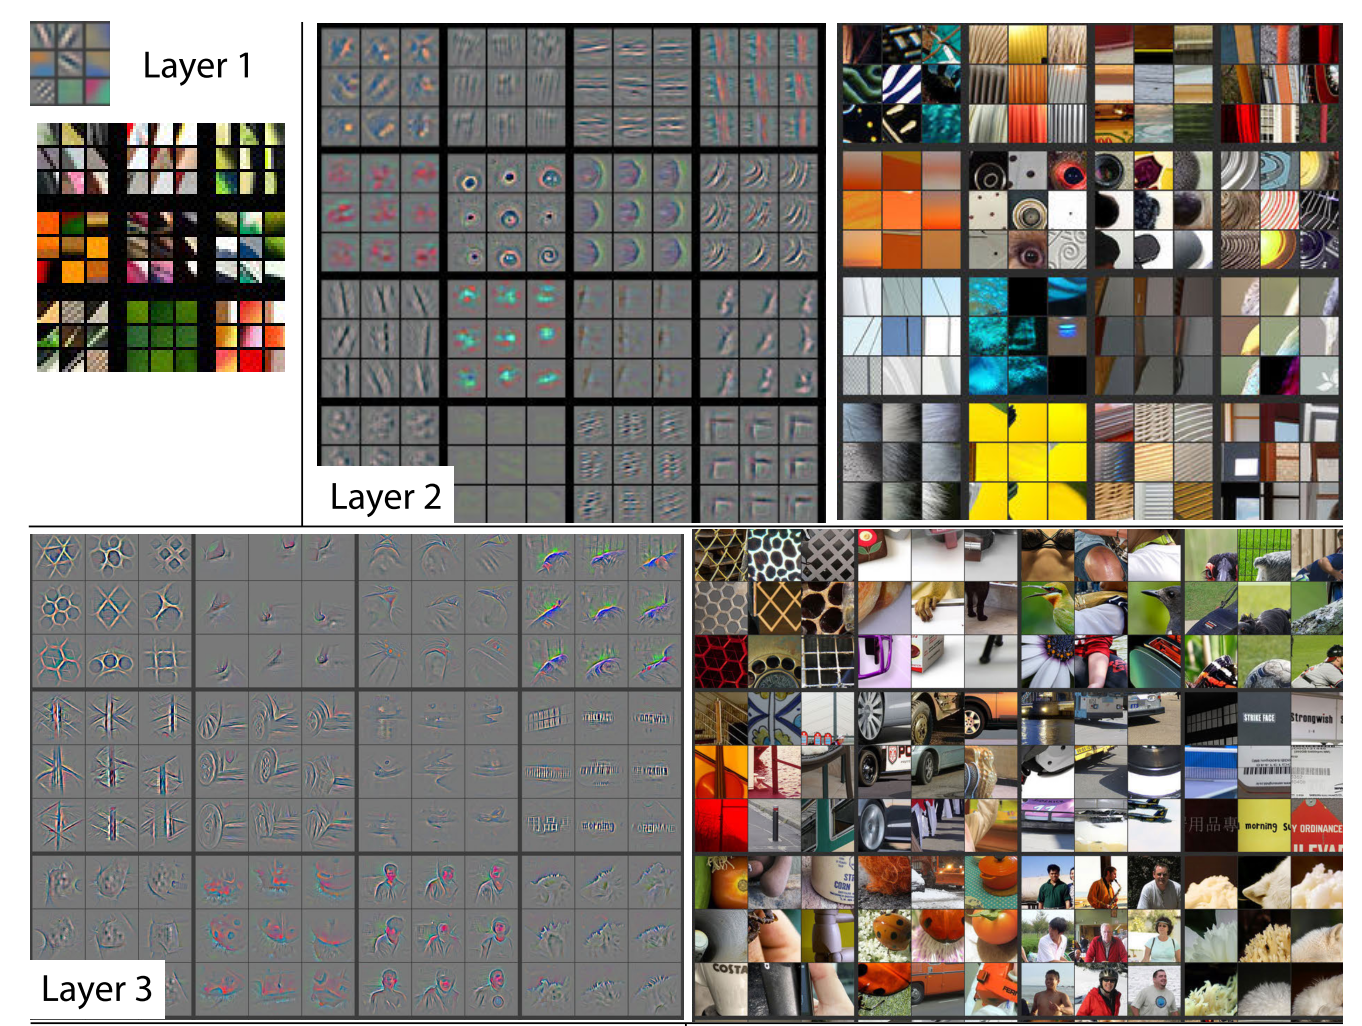
\includegraphics[width=0.5\textwidth]{img/zeiler_deconv.png} 
    			\caption{Zeiler Deconv}%
 		\end{figure}
 		
 		
		\par 
		\textbf{\cite{Erhan2009}} sought to find the optimal stimulation of a unit activations through gradient descent in the image space. This has been criticised as difficult to obtain due to the need for careful initialization, and the lack of information conveyed about a units invariance. 
		\par 
		\textbf{\cite{Le2010}} show how the Hessian of a given node may be computed numerically around an optimal response - thus fixing the formers shortcomings by providing a view of invariances. The issue with this approach is with the higher layers where invariances become increasingly complex and are thus poorly encoded in their quadratic approximations. 
		\par 
		\textbf{\cite{Vondrick2013a}} use feature inversion algorithms, where an image is featurized and then recovered to a transformed but decipherable format - again to give intuitive access to abstract feature representations formed by the network. Using this technique they discovered single deep neurons that were trained to respond to faces and bodies, both human and animal. 
		\par 
		\textbf{\cite{Zeiler2013}} provide a technique called \textit{Deconvolution} \cite{Zeiler2011} which effectively reverses a convolutional network. Deconvolution is a type of feature inversion that renders re-weighted versions of inputs, highlighting areas, patterns and textures of an image deemed most important by a particular part of the network. It essentially approximates a reconstruction of the input of each layer from its output.
		\par
		\textbf{\cite{Donahue2013}} show visualisations identifying patches in a dataset that cause strong activations at higher layers in a network. However these have been criticized as only producing a cropped version of the input images, so are limited learning tools. 
		\par 
		\textbf{\cite{Simonyan2013}} describe a technique for visualising class models learnt by CNNs. Given a CNN and a class of interest, the visualisation method numerically generates an image that is representative of the class in terms of the CNN class scoring model.
		\par 
		Clearly with such a lot of attention placed on visualising featurizations, it's a significant opportunity to learn about the networks. It's important to realise however that one of the above is not necessarily better than the others: each show a different element of the featurisation, and as experts still know relatively little about the behaviour of ANNs it's important to not discard any of these visual aids rashly.

\clearpage 

\section{Project Goals}
	To help guide development during the project a number of goals were identified. Over the course of the project the goals have been refined, new goals have been added and some goals have been dropped.
	\subsection{User Survey \& Interviews}
	\subsubsection{Survey Design}
	\par
	In order to help develop a set of refined goals for what was a broad goal - "Visualising Neural Networks"	 a survey was developed in collaboration with Jack Kelly to distribute amongst the Imperial College Staff known to be working with Neural Networks.
	\par 
	The survey was created and distributed to a small portion of those working closely with Neural Networks in relevant areas. The survey had a number of parts:
	\begin{itemize}
	
		\item \textbf{Describe your working environment}
		This had specific subtopics on languages used, packages familiar with and time taken to develop
		\item \textbf{Describe your training methods}
		This asked specifically about how often neural network design / architecture parameters were tweaked, which of those were considered to be most important, which were the most frustrating changes needed to be made and how they were currently solved.
		\item \textbf{Choose which visualisation technique you think is the most useful}
		The examples were shown of weights, gradients, activation mapping, architecture graphing, classification distribution and filters. 
		\item \textbf{Choose which element you think would be most useful to visualise}
		A list of all the different parameters that could be tweaked during training were given.
		\item \textbf{Do you currently visualise neural networks, and if so - how?}
		The question mentioned specific packages that are known to be commonly used amongst research communities and also asked about preferred method of interacting with the software. 
	
	\end{itemize}
	
	\subsubsection{Survey Results}
	\par 
	The results from the initial sample of researchers was very conclusive, and tied into my intuitions and my supervisors thoughts on the topic, and the fact that the number of researchers across Imperial was still relatively small for which this early survey would appeal - a second round of delivery was postponed in favour of product development and research into Neural Networks.
	\par

	\begin{figure}[H]
    			\centering												{{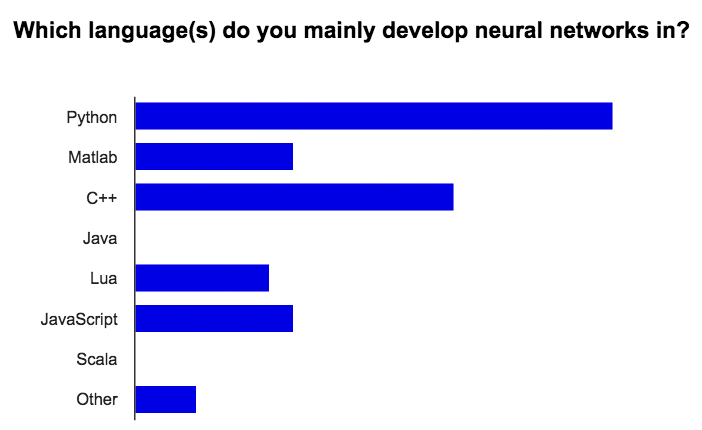
\includegraphics[width=7cm]
    				{img/survey-lang.png} 
    			}}%
	\end{figure}
	
	In response to working environment it was discovered that there was no package that researchers used any more than any other - and indeed single researchers would use multiple different neural network packages depending on the task at hand. For example: CUDA, Caffe, Lasagne, Torch and others. 
	\par 
	
	\begin{figure}[H]
    			\centering												{{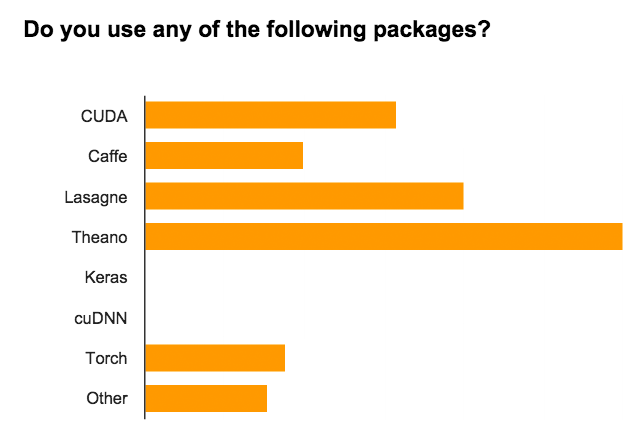
\includegraphics[width=7cm]
    				{img/survey-networks.png} 
    			}}%
	\end{figure}
	
	For some the tweaking of parameters and adjusting neural network architectures was the subject of whole PhD's - suggesting that tools that could help analyse the success of these changes could be invaluable to these researchers. 
	\par 
	Numerous methods were described for deducing the correct network parameters, or judging the quality of on set versus another. One researcher would get up on the screen various weight matrices from different training epochs upon a layer deep within the network and would simply switch tabs as fast as possible to try and observe changing numbers or patterns in the data - signs that the network would be training. 
	\par 
	
	\begin{figure}[H]
    			\centering												{{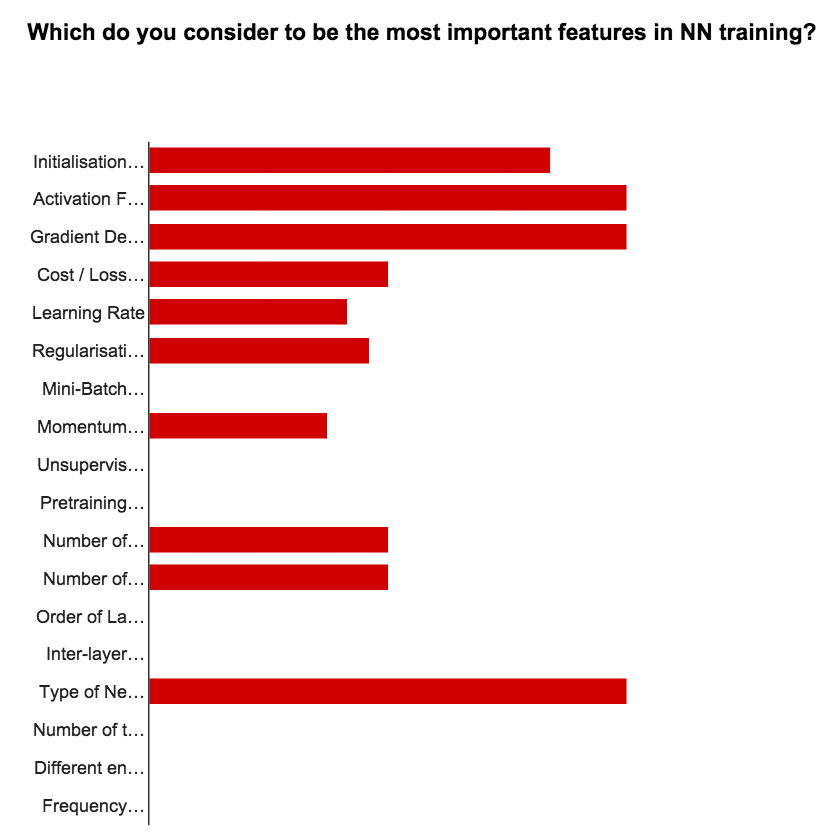
\includegraphics[width=7cm]
    				{img/survey-importance.png} 
    			}}%
	\end{figure}
	
	With respect to commenting on existing visualisations, it was surprising to see that most hadn't thought much about visualisation as a tool beyond graphing the commonly used error rates or accuracy. However were interested in the possibilities it might hold, and did respond when asked about which areas would be most useful.

	\subsection{Goals}	
	Through research into the problem of understanding neural nets, a number of goals were identified. After performing a review of existing software and distributing the survey, the process of constructing and refining a neural network and the network structure themselves the goals were refined. Some of the goals were achieved, however others arose once development had begun and as a result a number of goals were left incomplete. 
\\\
The initial goals were:
	\begin{itemize}
		\item \textbf{Improve existing capabilities}
		The purpose of this project is to improve the visualisation tools that are available to neural network researchers.
		\item \textbf{Provide Visualisations that take into account the domain}
			 This mean to create a more bespoke tool that can be used during the development of a functional neural network.
		\item \textbf{Visualise changing parts of the neural network}
			 Neural Networks, as explained earlier, have a fairly complex architecture. Individual neurons of different types form layers at different depths and with different numbers of units. Between these layers are weight matrices that change depending on the activations fired from neurons. These activations in the final sigmoid layer enable us to calculate a Validation Loss and Accuracy value. A visualisation tool would hope to visualise all of these changing parts to some degree or another. Not every element was implemented, however the majority are captured indirectly through the activations - which result in the other changes.
			 \item \textbf{Animation of this data} Having investigated the foundational theories of visualisation as proposed by Edward Tufte. Another goal of the tool is to enable the animation of the data, to show how the data changes over time. This way helping researchers to see how their models are learning - either in classifying the data better, worse or simply differently. This has been implemented in Iteration 1, and researchers can see how their networks classify data differently over time.
			\item \textbf{Investigate which visualisation combinations work best}
			The purpose of this goal was to try and discover if any visualisations would perform better than others when placed in the context of learning about neural networks. This goal has been achieved iteratively throughout the duration of the project, as each interaction develops on the combinations of visual elements that are needed to effectively help neural network researchers.
			\item \textbf{The ability to look at data from a number of different scales} 
			This goal is crucial in being able to understand both local and global patterns that emerge within the data. In iterations 2,3 \& 4 this goal has been satisfied.
			\item \textbf{Experiment data-mining}
			The purpose of this goal was to have some level of automatic data-collection from their network that would not interfere with their work flow. This goal has been implemented: researchers simply have call a function (API) within their neural network and the tool extracts the relevant information from the training network and stores it in Binary JSON (BSON) format using \textit{PyMongo}. This was only implemented after iteration 3 due to last minute server changes.
			\item \textbf{Provide full record of the network to revert back to successful networks}
			This goal has been implemented, and while the visualisation content is stored in a database. The crucial parameters of the current network are stored in both JSON and CSV format - a format that researchers are more comfortable working with. This enables researchers to reload models that were previously successful having analysed them, and to then make small adjustments.
			\item \textbf{making the data accessible}
			All data stored is very accessible, and while visualisation data (coordinates and their corresponding parameters) are available in the PyMongo database, easily accessed through a database interaction class. Regular Weights, Biases activations and other parameters are stored on file in formats that are easily accessible.
			\item \textbf{Realtime visualisation update} 
			This goal is clear, that as the neural network is training, the researcher can run the visualisation tool at any time to explore it's progress. The web server automatically uploads new information when the user selects a project.

	\end{itemize}	
	\subsection{Adjusting Expectations}
	While the majority of the goals stated in the previous session were achieved by the end of the project. Some of these were left partially complete - such as the "Visualise changing parts of the neural network" which while the final product would visualise a neurons activations and these directly influence the weights, biases, error values and accuracy - the product did not directly visualise anything other than those activations, which proved to be sufficiently useful and complex for the time of this project.
		
\clearpage
\section{Data Collection}
	
	The task of visualising neural networks primarily has three challenges to address; producing the data, collecting the data and visualising it. 
	\par 
	This chapter addresses the first two of those difficulties. In particular looking at the Neural Network implementations used, explaining the dataset and some considerations when collecting the data.
	
	\subsection{Neural Network Implementations}
	The purpose of creating a neural network in this project is not to create a unique implementation for a dataset that hasn't fully been explored yet. In fact quite the opposite - the implementations should be familiar enough to those looking into this study to enable them to partially ignore the networks producing the data, and instead understand the value of the visualisations that arise because of the network. Added complications in the network would only obfuscate the value of the visualisations. 
	
	\begin{figure}[H]
    			\centering												{{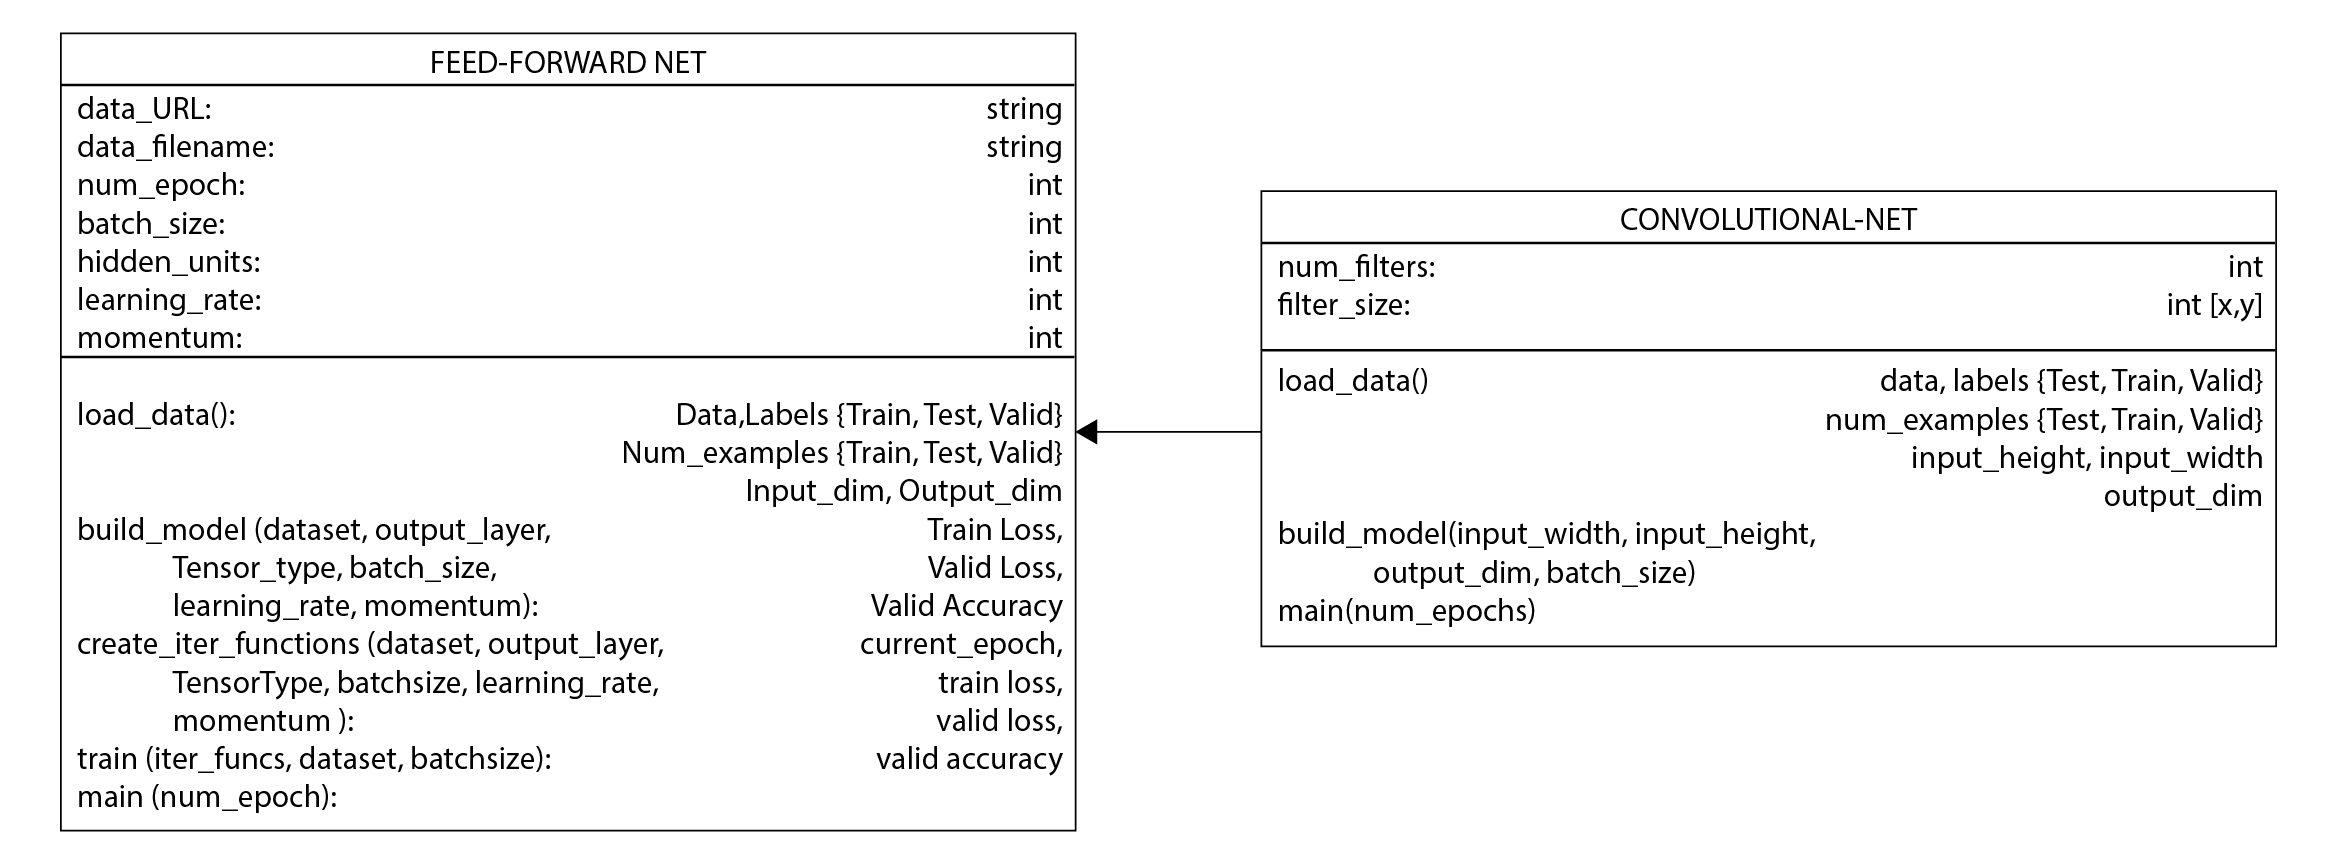
\includegraphics[width=0.7\textwidth]
    				{img/UML_nets.png} 
    			}}%
    			\caption{}%
	\end{figure}	


		\subsubsection{Feed Forward Net}

		In order to make the experimental network as close to industry standard as possible, the first neural network architecture is the same as that used in the classic Geoffrey Hinton 2012 paper in which he explains the concept of drop-out \cite{Hinton2012} - an idea that addresses a significant problem in machine learning - over fitting.
	
	\begin{figure}[H]
    			\centering												{{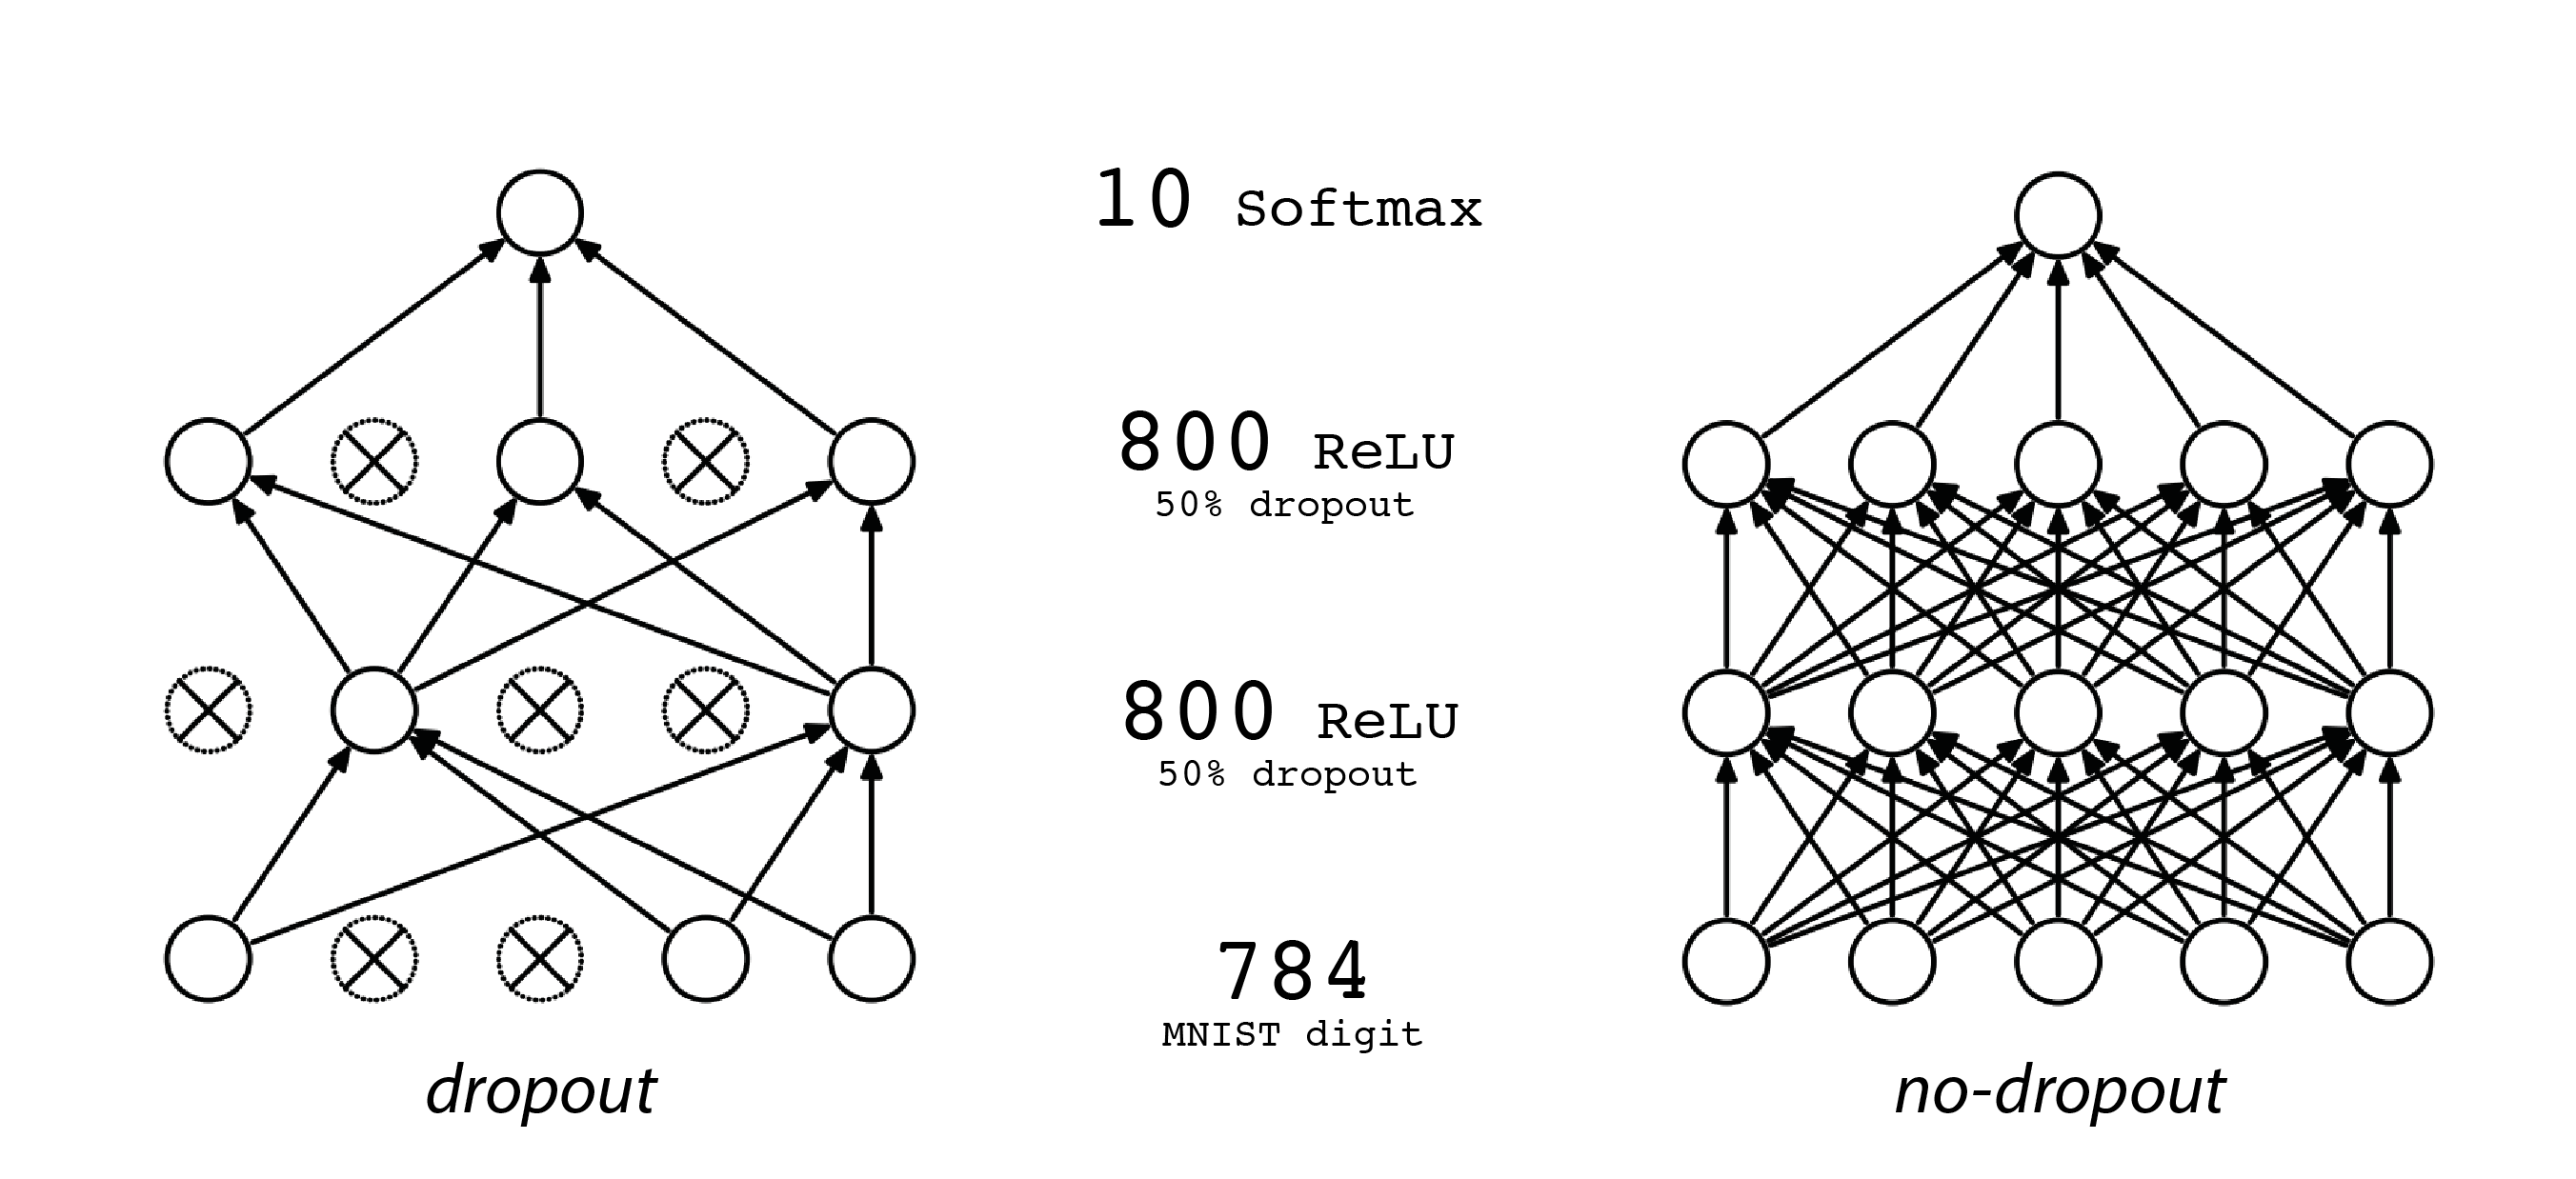
\includegraphics[width=12cm]
    				{img/hinton_dropout_2012.png} 
    			}}%
	\end{figure}

		\par 
		The network used takes 784-input values (the (28,28) images flattened into a single array) followed by two layers of 800 ReLU layers and the output Softmax layer of 10 (digits zero to nine). 
		\par 
		The other parameters used from the Hinton paper were a was 50\% drop-out between hidden layers and 100-sized mini-batches. However training did not follow the recommended 3000 epochs which, where the focus here is on visualisation and not on classification accuracy, was reduced to 100 for most tests, however some were experimented with larger samples and others with far fewer.
		\\\
		\subsubsection{Convolutional Net}
		\par
		Similarly to the Feed Forward Net, the aim was to use a well understood network. 
		\par 
		The Convolutional architecture used had the following structure at the beginning, which is a common adaptation of Yann LeCun's 1998 LeNet \cite{LeCun1998}: 
		\begin{itemize}
			\item Layer Input: (60000 [size of training set], 1, 28, 28 [dimensions of MNIST image])
			\item Layer 1: Convolutional Layer: 32 Filters, (3,3) Filter Size, (2,2) Pooling
			\item Layer 2: Convolutional Layer: 64 Filters, (2,2) Filter Size, (2,2) Pooling
			\item Layer 3: ReLU layer: 500 Units, 50% dropout
			\item Output: Softmax: 10 Units
		\end{itemize}
		\par 
		
		\subsubsection{Alteration}
		The above implementations are networks that are know to produce desirable results, or low classification error, this again does not fully satisfy the needs of this project.
		\par 
		One aim of visualising the networks is to understand when the networks have flaws, imperfections, quirks and other hopefully visually identifiable qualities. In order for us to demonstrate the value of the visualisation, the networks were broken in strategic ways. 
		
	\begin{figure}[H]
    			\centering												{{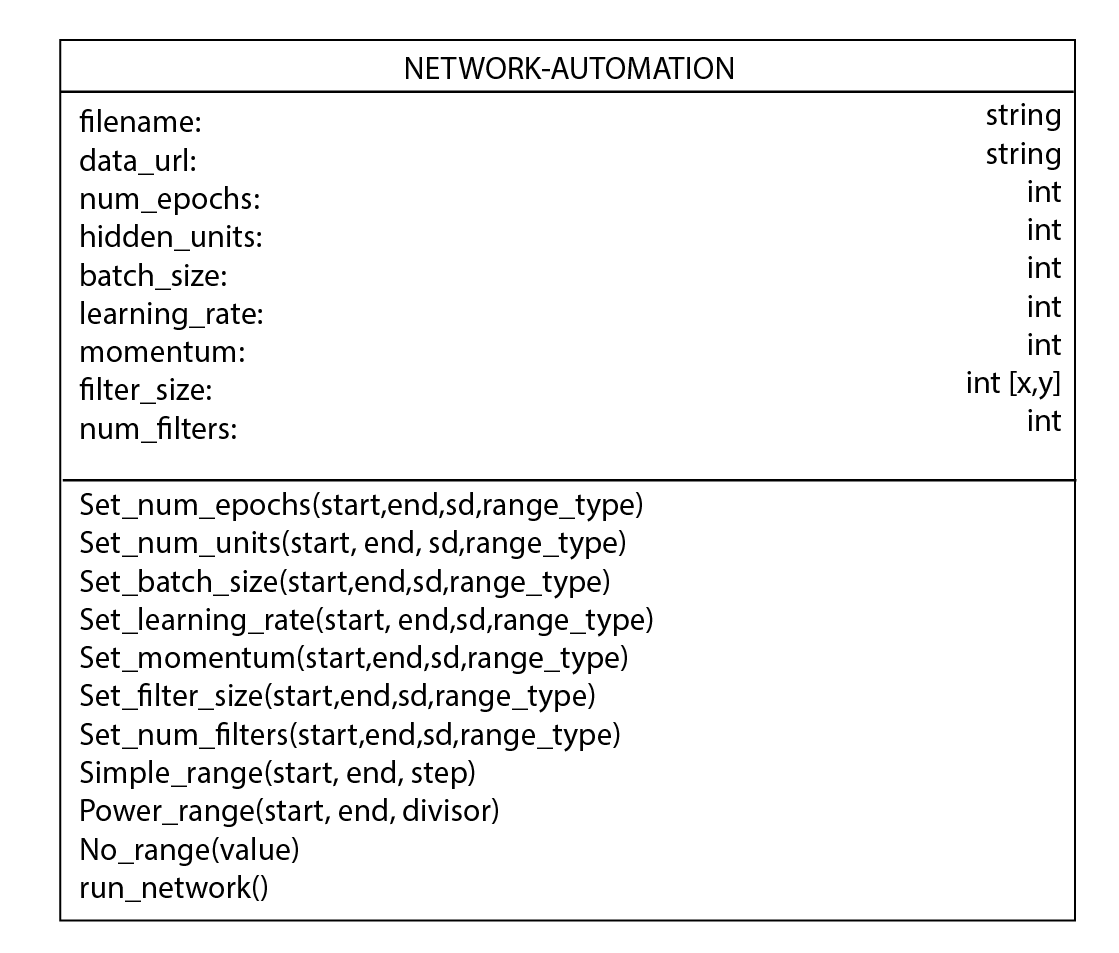
\includegraphics[width=0.5\textwidth]
    				{img/UML_auto.png} 
    			}}%
    			\caption{AutoNets}%
	\end{figure}	
	
		\par 
		For example a power range was defined that would run fewer experiments as it neared the understood value - \textbf{[1, 2, 3, 5, 7, 11, 17, 25, 38, 57, 86, 129, 194, 291, 437, 656]} - these values are examples run for the number of hidden units used within the networks. However other parameters were automatically tweaked including number of epochs, learning rate, momentum. Other parameters which required tweaking in the neural network code itself were only occasionally adjusted - such as the number of hidden layers, or type of non-linearity used.
							

		
		\subsubsection{Neural Network Implementation}
		The neural networks described above were implemented in a library designed for neural networks called \textit{Lasagne}.
		\par 
		Lasagne, is a neural network wrapper for the common machine learning python library \textit{Theano} which uses symbolic functions that compile at before runtime to ensure efficient mathematical processing. 
		\par 
		Lasagne was chosen after the survey of researchers revealed that the largest minority of users currently used Python implementations of neural networks. Theano could have been used, however was too detailed for the purposes of this project. 
		\par 
		It's important to note that in this incredibly fast moving field, the frontrunning technology is continually changing and throughout the course of this project another library \textit{Torch} has become increasingly popular due largely with it's ability to handle \textit{Recurrent Neural Networks} which haven't been mentioned in this report for simplicity reasons. 
	
	\subsection{Dataset}

	All experiments for this project were conducted using the MNIST dataset. There are a number of reasons behind this: firstly, the dataset is widely used as a  benchmarking dataset not just within neural network community but in the wider machine learning community as a whole; secondly, the dataset provides a useful base to test both a Feed Forward Network as well as a Convolutional Network - which should prove the value of the visualisation tool more so than attempting this on any one model architecture.
	
	\begin{figure}[H]
    			\centering												{{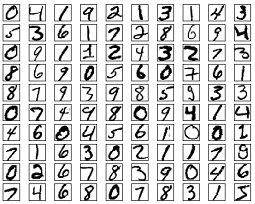
\includegraphics[width=7cm]
    				{img/mnist_digits.png} 
    			}}%
    			\caption{100 MNIST digits}%
	\end{figure}
	
	The dataset itself contains 60,000 training images and 10,000 test images. Each image is a 28 pixels by 28 pixels hand-written digit from one to nine.
	\par 
	It's important to recognise that for the purposes of testing this tool for research the MNIST dataset provides a quick set to train upon. While the CIFAR datasets would provide more interesting analysis and represent a more realistic task - such as image recognition - the MNIST dataset is simply one list of intensity values in comparison the the three Red, Green and Blue of the CIFAR set. The below images demonstrate the simplicity of the dataset.

	\begin{figure}[H]
    			\centering	
    			\subfloat[MNIST digit]								{{
\includegraphics[width=0.2\textwidth]
    				{img/mnist_four_image.png} 
    			}}%
    			\qquad
    			\subfloat[Intensities]																			{{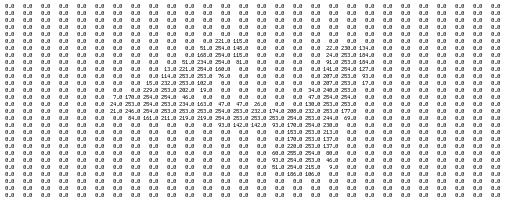
\includegraphics[width=0.5\textwidth]
    				{img/mnist_four_intensities.png} 
    			}}%
    			\caption{}%
    			\label{fig:mnist_four}
		\end{figure}

	\subsection{Collecting Output Data}
	
	\subsubsection{Data Collection Goals}
	\par
	There were a number of requirements to fullfill when collecting the data:
	
	\begin{itemize}
		\item Data that will be used online must be stored in a compact format. This was achieved using a MongoDB database which stores JSON objects in binary, in the later iteration of the project using the python library \texttt{pymongo}.
		\item Data that researchers use to assess the quality of their models should also be stored in a common format that can be easily interrogated. This was achieved by using Pythons sophisticated \texttt{sys} and \texttt{os} packages.
		\item Data from the neural networks must retain it's shape for easy importing with the python library \texttt{numpy}.
		\item Image data must be stored in a more compact format that integers of intensity or RGB value due to the vast size. This is achieved by preprocessing image data with the python library \texttt{base64} which compresses the images into a Float32 array in base64 notation - which then usefully becomes small enough to store in the \textit{Mongo} database.
		\item Coordinate data for the scatter plots must be stored in a condensed form that allows easy iteration over within \textit{d3.js}. (500, 2) matrices are therefore \texttt{numpy.reshaped} to (1000,) single dimension arrays.
	\end{itemize}
	
	\subsubsection{Structuring the data}
	Within neural networks there are several moving parts, and with those tremendous amounts of data that can be collected during pre-training, training and during the testing phases. 
	\par 
	It was important to fully understand these components in order to effectively store the data outputted from the neural networks in a suitable database. The following entity relationship diagram demonstrate the majority of the moving parts that this project is concerned with, and in fact covers the majority of the neural network parameters and data that can be collected. 
		
	\subsubsection{Collecting the data}
	\par 
	In order to process the data in accordance with the above goals, a library of python functions was developed that could be imported with ease into the neural network itself.
	\par 
	These functions effectively create an easy to use API for connecting the neural network to two main methods of storage - the file system storage that enables researchers to examine their data first hand, and the database storage that stores only those pieces of information important for the visualisations. 
	\par 
	The functionality behind this data collection was implemented at first using pythons \texttt{os} and \texttt{sys} libraries that enable the user to save directly into their file directory. While early on in the process a complex database implementation was created following the below entity relationship schema for the \textit{Node.js} back-end, and \textit{MongoDB} database - the \textit{MongoDB} collection was later simplified to make it easier for researchers to interact with the database. In addition the database was moved from \textit{JavaScript} to \textit{Python} using a \textit{MongoDB} wrapper \textit{PyMongo} to ensure that the back-end processing was entirely in Python.
	
	\begin{figure}[H]
    			\centering												{{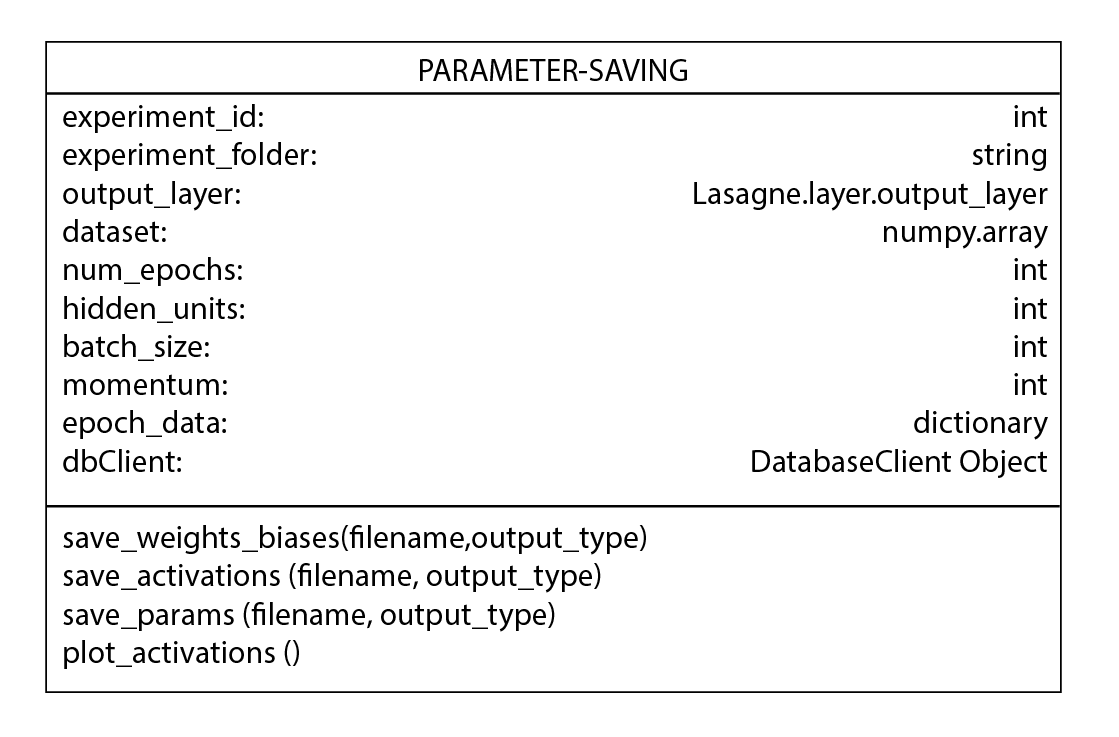
\includegraphics[width=7cm]
    				{img/UML_saving.png} 
    			}}%
    			\caption{Saving Functionality}%
	\end{figure}		
	
	\begin{figure}[H]
    			\centering												{{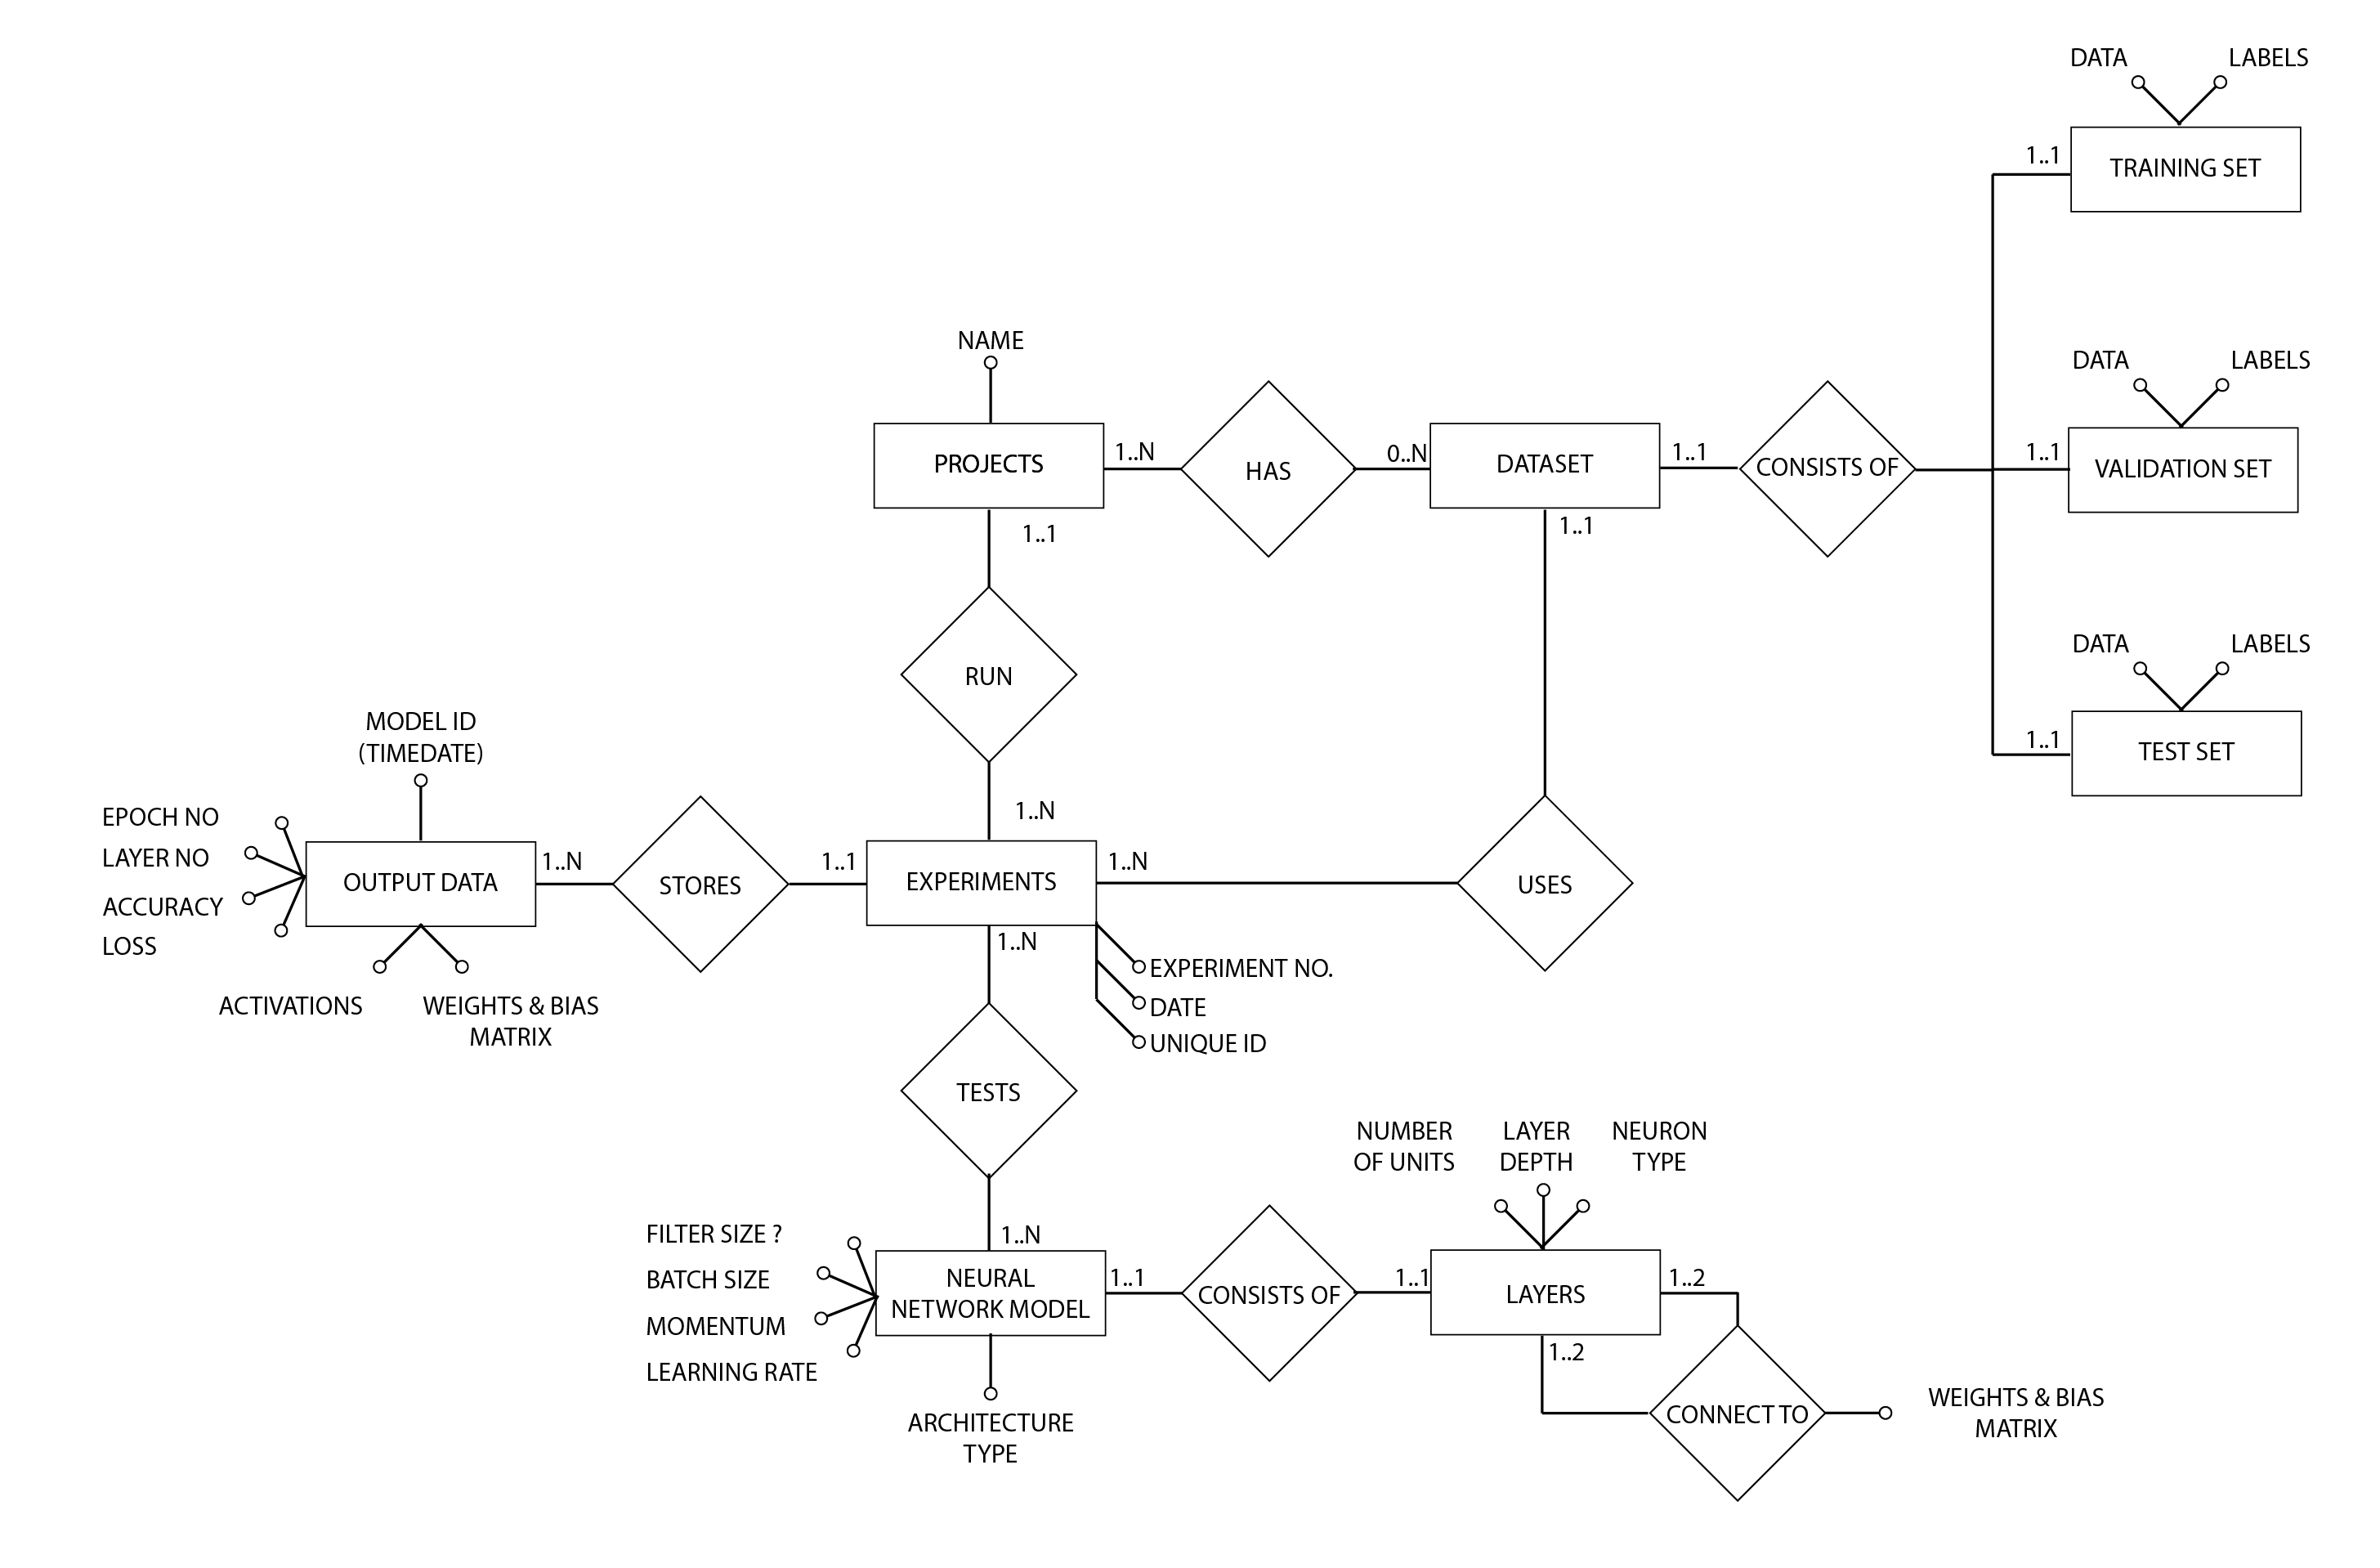
\includegraphics[width=17cm]
    				{img/ER_horiz.png} 
    			}}%
    			\caption{Initial ER diagram}%
	\end{figure}	

	
\subsection{Evaluation}
The aims of this first section was to explain to the reader the foundation upon which this project was built. Namely, two well understood neural networks that get tweaked in various ways away from parameters that ensure optimal performance. This is done in order to try to understand better how poor networks may appear when visualised. The section also explains the importance of gathering the data outputs of these networks in an appropriate fashion, and the importance of choosing the MNIST dataset. 
	\par 
	With a basic understanding of the neural networks and dataset used, and an understanding of the data collection methods, the remainder of the report will explore how that data can be visualised and what is significant about this.

\clearpage
	
\section{Dimensionality Reduction}

Neural Networks are famous for ability to comprehend complex datasets such as vision or speech. These datasets are often complex for one primary reason - the data contains very high dimensionality.

 	\begin{figure}[H]
    			\centering	
			{{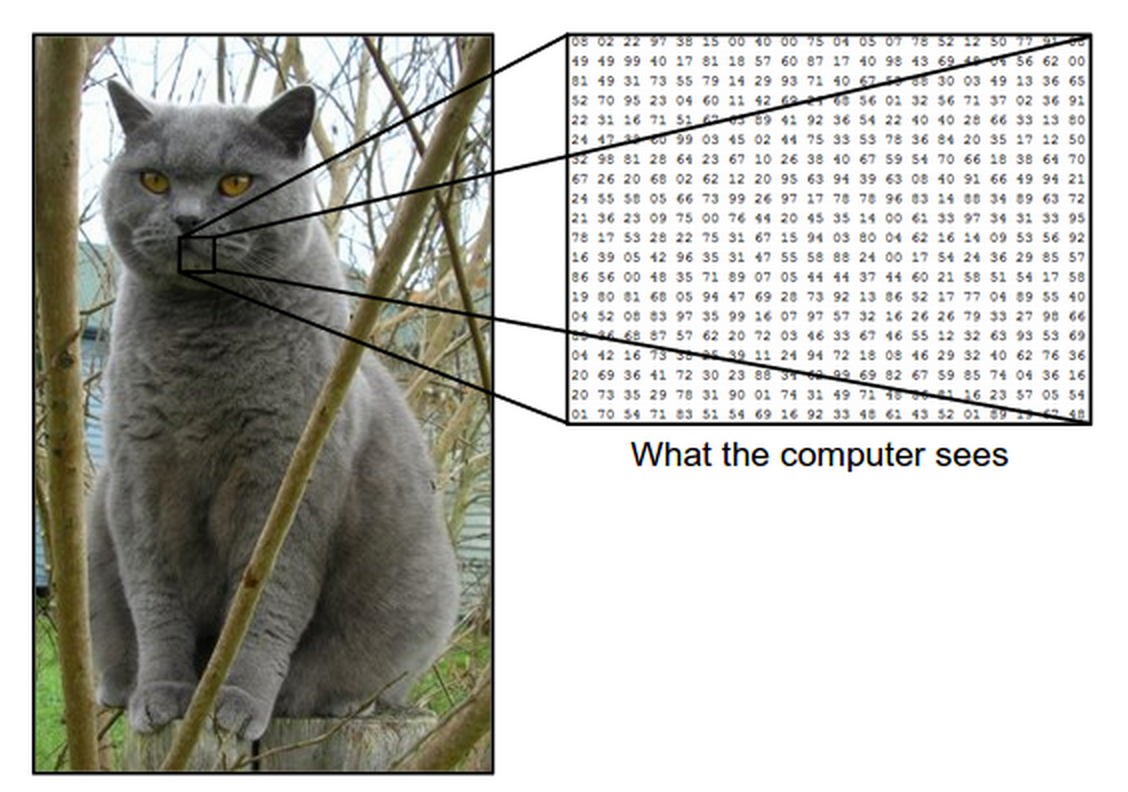
\includegraphics[width=0.45\textwidth]
    				{img/catimage.png} 
    			}}%
    			\caption{Cat}%
    		\label{fig:lascaux}
	\end{figure}
	
	The image above is 248 pixels wide, 400 pixels tall, and has three colour channels Red, Green and Blue - which to the computer is stored in a multidimensional array of dimensions (248,400,3) or 297,600 numbers. When this image is passed into the computer it understands this data as 297,600 different data points - not as a cat.
	\par 
	As this image passes through a neural network, the number of dimensions (248,400,3) changes to make it easier for the network to classify this image as a cat - one of 10 classes in the CIFAR-10 dataset. So while a human can understand this image as a cat, when the data is transformed say to (512,20,2) dimensions the cat is no longer recognisable to to - but to a computer, may be more 'cat-like'.
	\par 
	These later dimensions are defined by the activations that a layer of neurons produces in response to being passed the weight-transformed cat image. It is these dimensions that we are interested in, and give us an insight into how successfully our neural network is training. 
	\par 
	In order for use to visualise this information in a way that is understandable to the human brain (and therefore useful as a diagnostic tool), we cannot simply show the numbers - we must map these numbers to a smaller number of dimensions that we as human beings are incredibly good at understanding - our 3 spatial dimensions. 
	\par 
	This section will explore the notion of both visualising high-dimensional data, where the aim is to retain data fidelity and show all the data points, and the notion of dimensionality reduction - where we reduce the number of dimensions mathematically.
\\\
\subsection{Visualising High-Dimensional Data}
	Visualising high-dimensional data is a very important problem in several different domains that each deal with data of widely varying dimensionality. It is therefore a very well explored problem and a number of techniques for visualising high-dimensional data exist, a summary of which was composed by \cite{Cristina2003}.
	\par 
	This covers techniques by a number of different authors that could be useful for the visualising of neural network data;	
		\par
		
 	\begin{figure}[H]
    			\centering	
			{{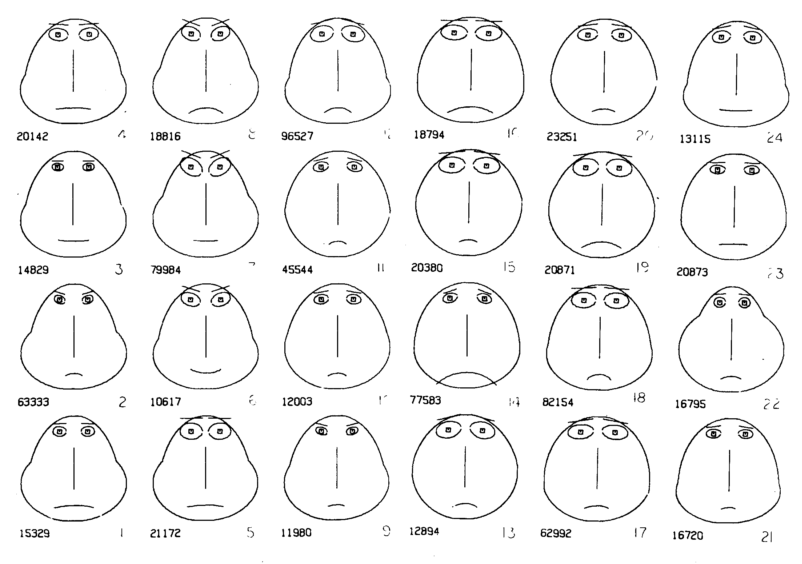
\includegraphics[width=0.3\textwidth]
    				{img/chernoff_faces} 
    			}}%
    			\caption{Chernoff Faces}%
    		\label{fig:lascaux}
	\end{figure}
 		
		 \textit{Chernoff Faces} are iconographic visualisations of faces by \cite{Chernoff1973}; each point in k-dimensional space, $ k < 18 $, is represented by a cartoon of a face whose features, such as length of nose and curvature of mouth, correspond to points in the data. Thus every multivariate observation is visualized as a computer-drawn face. This presentation makes it easy for the human mind to grasp many of the essential regularities and irregularities present in the data. Looking at the faces it's easy to see which data points are similar and with which parameters - such as those faces with larger eyes would represent similarities across a common dimension. This technique is not useful for most neural networks which have greater that 18 dimensions.
		 \par
 		
 	\begin{figure}[H]
    			\centering	
			{{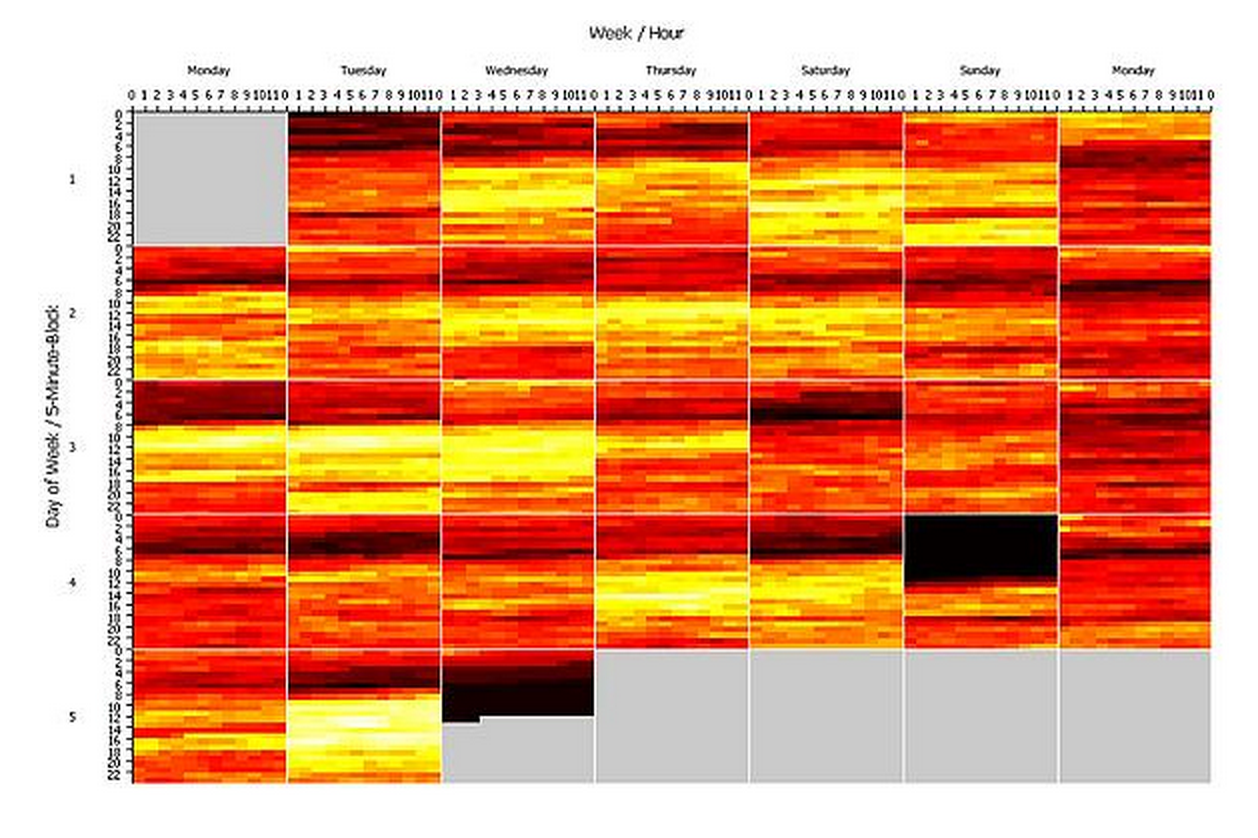
\includegraphics[width=0.3\textwidth]
    				{img/kiem_pixel_two} 
    			}}%
    			\caption{Pixel Based Techniques}%
    		\label{fig:lascaux}
	\end{figure}	
 		
		\textit{Pixel Based}; represent as many data points as possible on the screen at the same time by mapping each data value to a pixel of the screen and rearranging those pixels to suit the source \cite{Keim2000}. One example is to use a gradient of colour to represent the value of a data-point, and multiple dimensions may be show in different as slices tiled together.
		\par 
		 		
	\begin{figure}[H]
    			\centering	
			{{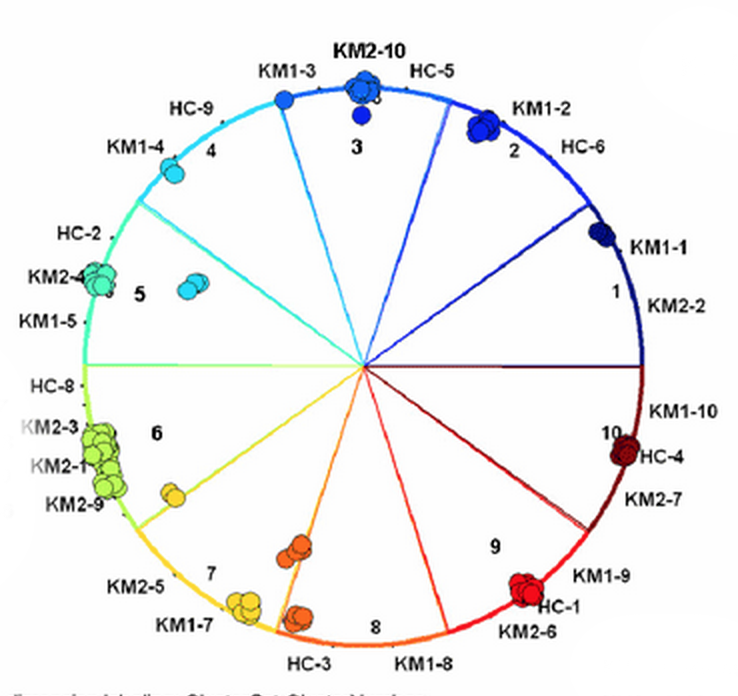
\includegraphics[width=0.3\textwidth]
    				{img/battista_vertices} 
    			}}%
    			\caption{RadViz}%
    		\label{fig:lascaux}
	\end{figure}	 		
 		
 		
		\textit{Radial Coordinate Visualisation} was designed by\cite{Hoffman1999}; which for an n-dimensional visualisation, n lines emanate radially from the center of a circle and terminate at its perimeter, each line is associated with one attribute. The points that sit in amongst the radial portions represent the data described between the dimensions in a way that is similar to an x-y plot.
		\\\
		\\\
	While these tools do have their uses as visualisation techniques, when it comes to exploring the high-dimensional data of neural networks they have been criticized \cite{Maaten2008} as simply providing the tools to \textit{display} more than two data dimensions, and leave a more difficult task of interpretation to the viewer. With the number of dimensions using in real-world neural networks often in the thousands, these techniques may provide limited insight, and so it's important to look in detail instead at Dimensionality Reduction which does some of the data interpretation for us.
\\\

\subsection{Dimensionality Reduction}
	Dimension reduction differs from dimensionality visualisation, in that instead of visualising the multiple dimensions of a dataset in a format such as those already described, it actually converts the high-dimensional data set  $ X = \{ x_{1}, x_{2},..., x_{n} \} $ into a low-dimensional data set that can then be displayed easily in a standard recognisable formats such as the scatter plot. Dimensionality reduction aims to preserve as much of the significant structure of the data in higher-dimensions as possible while generating a low-dimensional representation that is easier for the user to interpret. This is fundamentally important for visualising neural nets where activations are often many thousands of dimensions.
		\par 
		It has been suggested by \cite{Olah2014b} that it is possible to draw a notion of how successful this dimensional reduction is by assuming that for any two data points, $ x_{i} $ and $ x_{j} $ there are two notions of distance between them that we can compare. First, is the distance between those points in the real world space, for example the L2 distance $ d(x_{i,j}) = \sqrt{\sum\nolimits_{n} (x_{i,n} - x_{j,n})^2 } $, and the other is the  distance between the points in the visualisation, $ d_{viz}(x_{i,j}) $, such that a cost function of the visualisations success can be defined.
		\par  		
		If the cost $ C $ is high, then the distances are dissimilar to the original space, if low they are similar, and if zero the visualisation is a perfect representation. It's almost impossible however to get a perfect representation in all aspects, so different cost functions provide different compromises, and insights. Once the cost function is designed there simply exists an optimisation problem that can be tackled though a standard process such as gradient descent to ensure that points are optimally visualised with respect to the cost function. The cost function for standard Multi-dimensional Scaling \cite{Torgerson1952} is shown below: 
		$$
			C = 
			\sum\limits_{i \neq j}
			[d(x_{i,j}) - d_{viz}(x_{i,j}) ]^2
		$$
		\par 
		Another reduction method is Sammon's mapping \cite{Sammon1969}, which aims harder to preserve the distances between nearby points than those further away. If the two points are twice as close in the original space than  two others, it is twice as important to maintain the distance between them. This emphasises the local structure at the compromise of the global structure in the data:
		$$
			C = 
			\sum\limits_{i \neq j}
			\frac{ [d(x_{i,j}) - d_{viz}(x_{i,j}) ]^2 }					{d(x_{i,j})}
		$$
		A number of other techniques were reviewed by \cite{VanderMaaten2009} who describes \textit{Principle Components Analysis, PCA,} \cite{Hotelling33} - which finds the angle that spreads out the points the most in order to capture the largest variance possible, and \textit{Multidimensional Scaling} as seen above - as linear techniques that keep low-dimensional depictions of dissimilar points far away, but which fail to keep those data-points which are similar close together in the lower dimensional depiction.
 		
 	\begin{figure}[H]
    			\centering	
			{{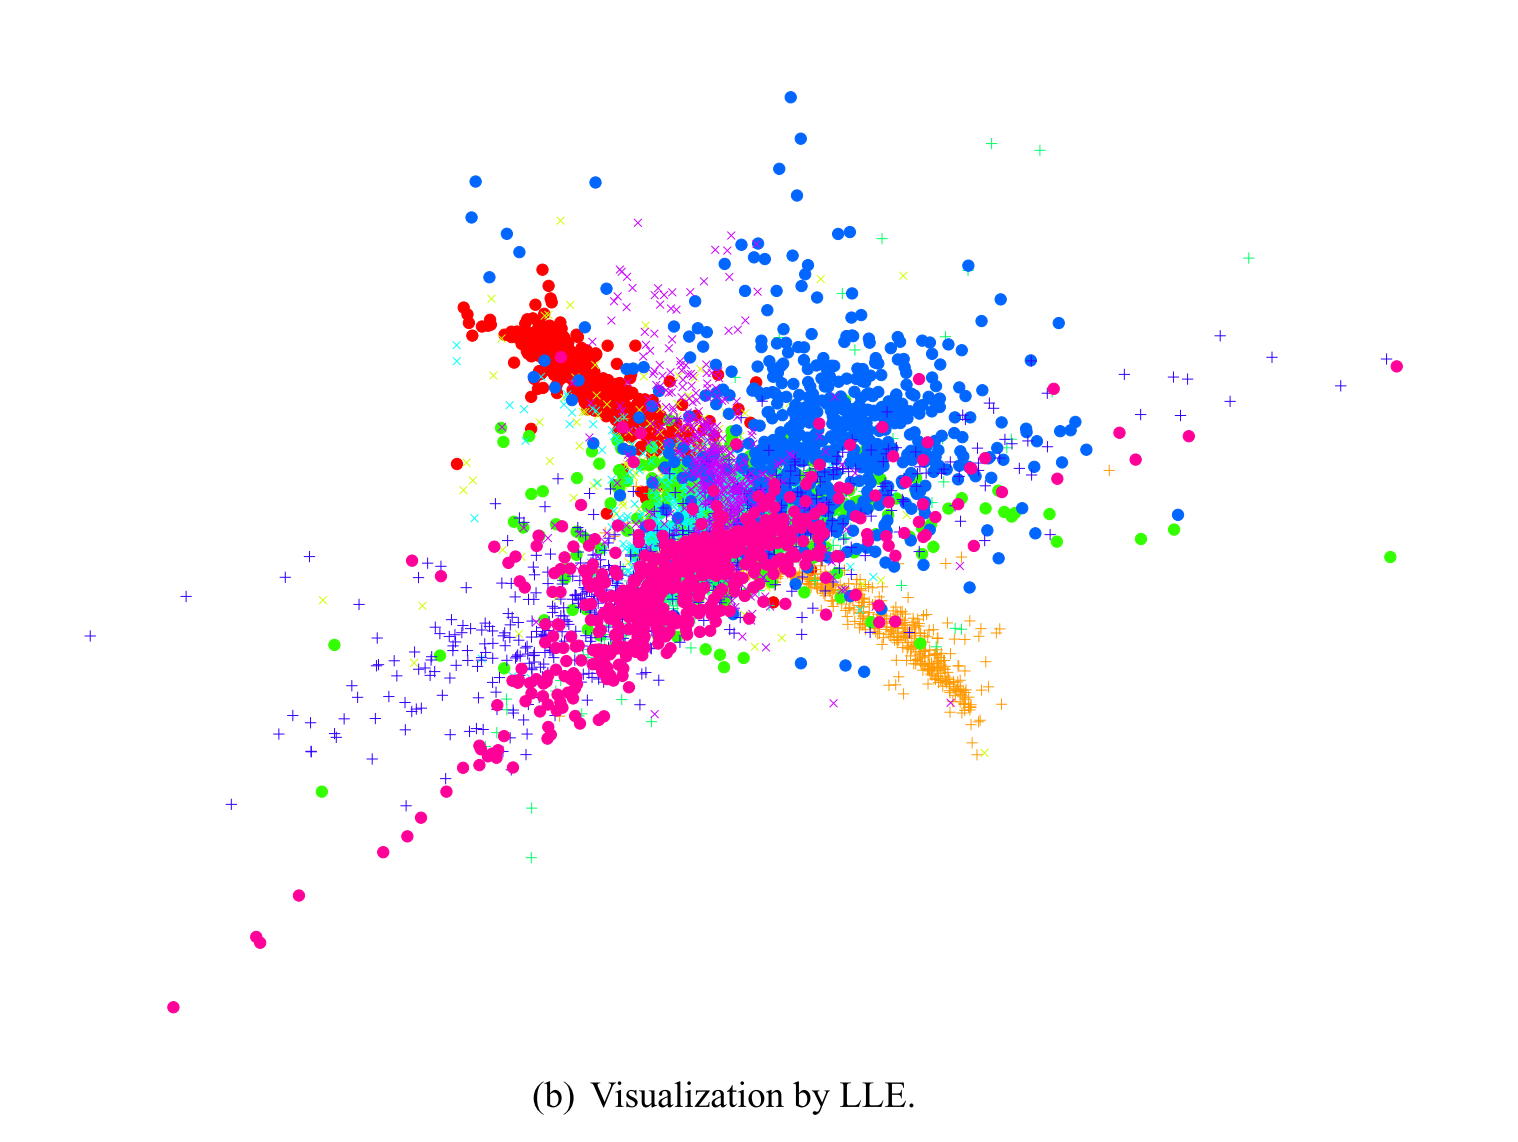
\includegraphics[width=0.3\textwidth]
    				{img/hinton_lle.png} 
    			}}%
    			\caption{MNIST - a Locally Linear Embedding}%
    		\label{fig:3nn}
	\end{figure}	 
 		
		\par 
		In addition to Sammons mapping described above, \cite{VanderMaaten2009} also sites a number of other non-linear dimensionality reduction techniques that aim to preserve the local structure of data including; \textit{Curvilinear Component Analysis} \cite{Demartines1995}, \textit{Stochastic Neighbour Embedding} \cite{Hinton2002}, \textit{Isomap} \cite{Tenenbaum2000}, \textit{Maximum Variance Unfolding} \cite{Weinberger2004}, \textit{Locally Linear Embedding} \cite{Roweis2000}, \textit{Laplacian Eigenmaps} \cite{Belkin2002}.

		\par 
		
		These techniques all perform well with artificial datasets, however are criticised for not being capable of retaining both local and global structure in a single data map. Even semi-supervised variants are not capable of separating simple datasets such as MNIST into it's natural clusters \cite{Song2007}. 
		\par 

	 		
 \subsection{t-Distributed Stochastic Neighbour Embedding}
		More recently, and in direct challenge to those mentioned earlier, \textit{t-Distributed Stochastic Neighbour Embedding} \cite{Maaten2008} has provided a successful and widely used alternative for neural network researchers. tSNE, as it is abbreviated, captures much of the local structure of high-dimensional data, while also revealing global structure such as the presence of clusters at several different scales.
		\par 
		
	\begin{figure}[H]
    			\centering	
			{{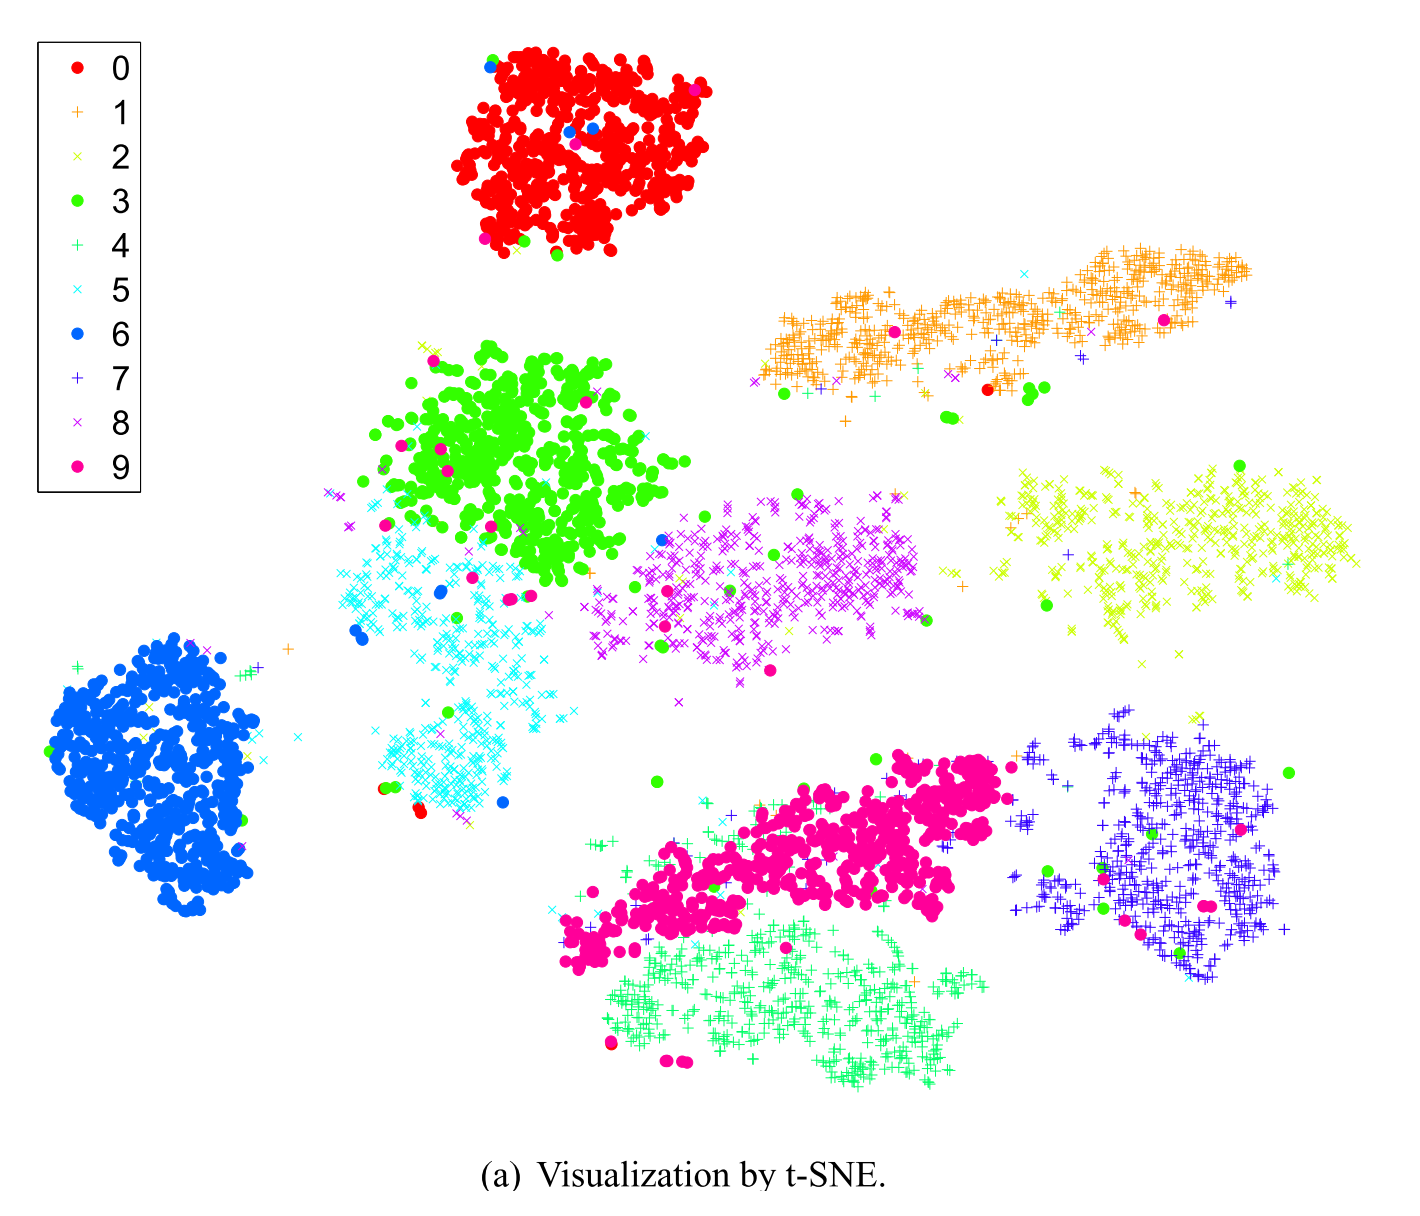
\includegraphics[width=0.3\textwidth]
    				{img/hinton_tsne.png} 
    			}}%
    			\caption{tSNE}%
    		\label{fig:3nn}
	\end{figure}	  
	
	
		tSNE can therefore be viewed as preserving the topology of the data. tSNE constructs for every data point a notion of which other points are it's `neighbours' and tries simultaneously to ensure that all points in the data have the same number of neighbours. tSNE is a lot like a nearest-neighbour graph, however instead having a set number of neighbours connected by edges, and non-neighbours for which there are no connections, data points in the tSNE reduction have a continuous spectrum of neighbours, for which they are neighbours to different, non-binary, extents. This makes tSNE very powerful in revealing global clusters and local sub-clusters within the data - which is ideal for working with complex neural network activations that should display a sophisticated understanding of both.
		\par
		 The one downside of tSNE is that it's prone to getting stuck at local minima, and due to it's increased complexity is more computationally expensive to run, such that changes cannot be made and visualised in real time on standard machines and can take any number of hours, or days even, to produce.  
	\subsection{Evaluation}
	Not one of the dimensionality reduction techniques mentioned appears to be superior. They are largely complimentary, and choice of which to use intuitively depends on the needs of the data-set and the visualisation scenario. 
	\par 
	Each has it's own trade off in order to preserve the most important properties for it's unique scenario. This is potentially obvious as there can be no exact mapping from high-dimensional space to low dimensional space. 
		\par 
		PCA preserves linear structure, MDS preserves global geometry and tSNE tries to preserve a topological neighbourhood structure.
		\par 
		For the remainder of this project data produced by the neural networks will be reduced in dimensions using the tSNE algorithm, or a faster derivative thereof. The reasons behind this are that when looking into neural networks it is unclear what exactly we are looking for, be it variance, local structure, global structure, or some unknown. tSNE preserves the overall topological structure and thus provides a good solution when looking into the data generated by the neural nets. In addition, tSNE has been used incredibly successfully used in the past by some leading neural network researchers to visualise their data\cite{Maaten2008}.
		\par 
		Not only does tSNE satisfy several important criteria for enabling us to understand the high dimensionality of neural network data, but it also allows us to meet a number of Edward Tufte's theories of good visualisation:
		\begin{itemize}
			\item tSNE dimensionality reduction helps the visualisations meet Tufte's first principle \textit{"show only as much information as is required"} in comparison to the dimensionality visualisation. In the former, vast amounts of data is compressed to reveal just enough information to enable us to make useful judgements, where as in the latter we are likely showing far more data than is required, thus breaking Tufte's first rule.
			\item By transforming the non-visual information (numerical activation values) into two dimensional points through the tSNE algorithm, we have placed the data in a format that lends itself to classic visualisation in the x-y dimension - a scatter plot. This satisfies Tufte's third principle tapping into the human brains innate ability to understand spatial patterns.
			\item tSNE also explicitly follows Tufte's fourth principle of good data visualisation that, \textit{differences in visual properties should correspond to actual difference in the data}, by in it's very aim which is to optimise a cost function that aims to preserve the actual differences in the data (here described using metrics such as the L2, or Euclidean, distance).
		\end{itemize}
		It has been suggested that one reason for the success of neural networks is that they discover optimal representations of the data that allow for more accurate classification \cite{Hinton1986}. Ultimately understanding these better should provide a method to guide the training process that is less situated in trial and error.
		\par
		 Importantly, these representations are likely to be distributed \cite{Hinton1986} such that each concept is encoded in the activations of any number of the networks nodes, making understanding these concepts a greater problem than simply understanding the decision surface on singular neurons, but one that requires representations across all nodes.
		 \par 
	In the input space the network requires a relatively complex line to divide two curves on a plane. However each new layer transforms the spatial data creating a new representation that is easier to classify with a simple hyperplane.
				
		\begin{figure}[H]
    			\centering	
    			\subfloat[No hidden layer]							{{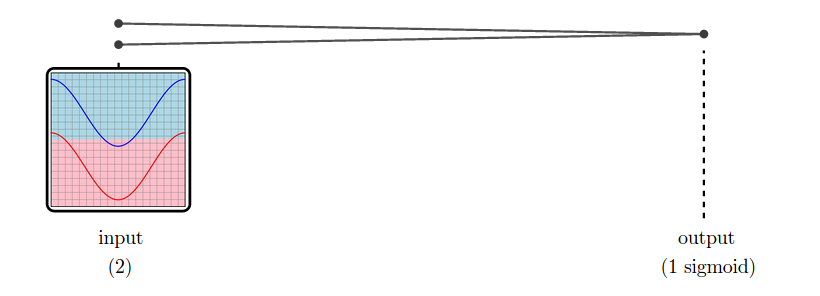
\includegraphics[width=7cm]
    				{img/colah_nonwarp.png} 
    			}}%
    			\qquad
    			\subfloat[Hidden Layer]
    			{{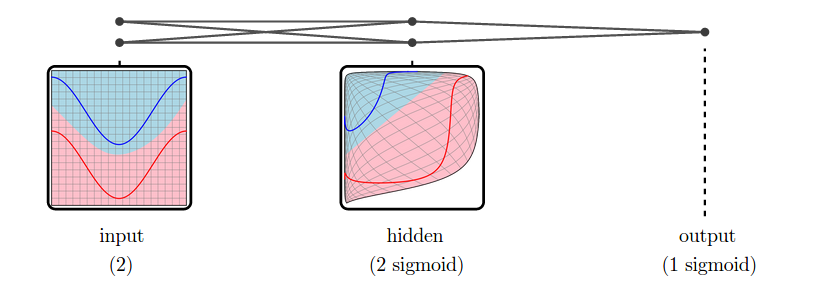
\includegraphics[width=7cm]
    				{img/colah_warp.png} 
    			}}%
    			\caption{Representations that warp the data}%
		\end{figure}		
		
		\par 
		In order for the data to be transformed to this new representation, it must undergo a sequence of manipulations. A tanh layer for example processing the function $ tanh(Wx + B) $ consists of; 
		\begin{itemize}
			\item a linear transformation by the weight matrix $ \bm{W} $
			\item a translation by the bias vector $ \bm{b} $
			\item and a point-wise application of the tanh activation function
		\end{itemize}
		Intuitively, what is occurring here is a stretching and warping of the space to make it easier to linearly divide and this can be seen above as well. It's important to note however that it does not cut, break or fold the space as it must retain it's `topological' properties \cite{Choi2005}.
		\par 
								
 		 \begin{figure}[H]
    			\centering													{{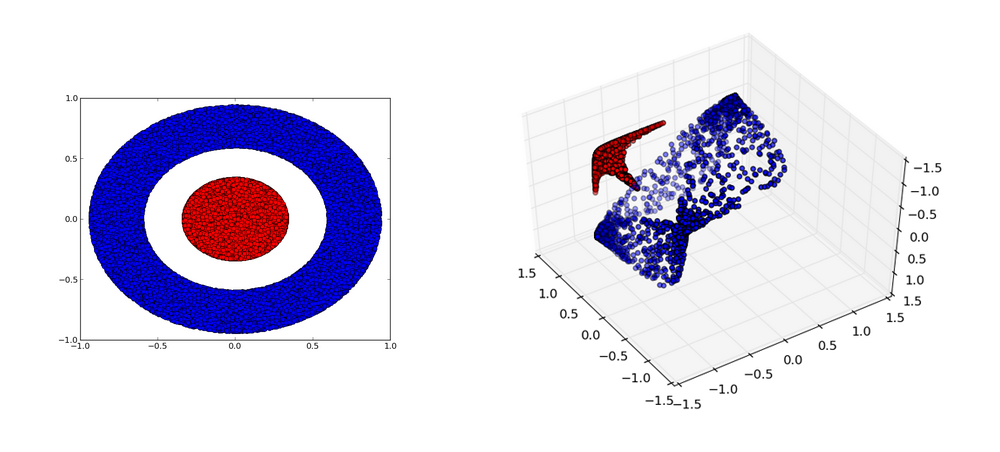
\includegraphics[width=0.6\textwidth]
    				{img/colah_circle} 
    				}}
    			\caption{Three Node Warping}%
    			\label{fig:studentprofile}
		\end{figure}
		
 		
		Another example, is one that cannot be warped simply in two dimensions, but requires a third, such as a circle within a circle:
		$$ 
		A = \text{ $ { xld(x,0) < 1/3 } $ }		
		B = \text{ $ { xl2/3 < d(x,0) < 1 } $ }
		$$ 
		It is impossible for a neural network to classify this without having a layer with greater than 3 hidden neurons. The requirement of the network to find a hyperplane that separates $ A $ and $ B $ in some final representation will not be possible no matter how the space is warped - the network requires an extra dimension. Visualisation demonstrates the network struggle to perform this. However, if we add a third  neuron, the problem becomes trivial - with a three dimensional representation of the data. This spatial transformation occurs in even more complex datasets with numerous dimensions \cite{Carlsson2008} such as images. however, while it is less easy to visualise these the intuition is useful and may lead to discovering appropriate ways of showing the same transformations in multi-dimensional space.
\clearpage

\section{Iteration 1 - Animation}
	\subsection{Introduction}
	Reducing the dimensionality of our data is in itself not enough. 
	\par 
	While it is possible to simply plot as much of the data as possible, the sheer quantities of tSNE plots would quickly put us back in the first positions - being unable to compare data due to information overload, potentially requiring us to reapply tSNE. 
	\par 
	Instead by looking back to Edward Tufte's principles of visualisation and observing those which we have not achieved, the solution becomes immediately obvious: animate the data.
	\par 
	
	\begin{figure}[H]
    			\centering												{{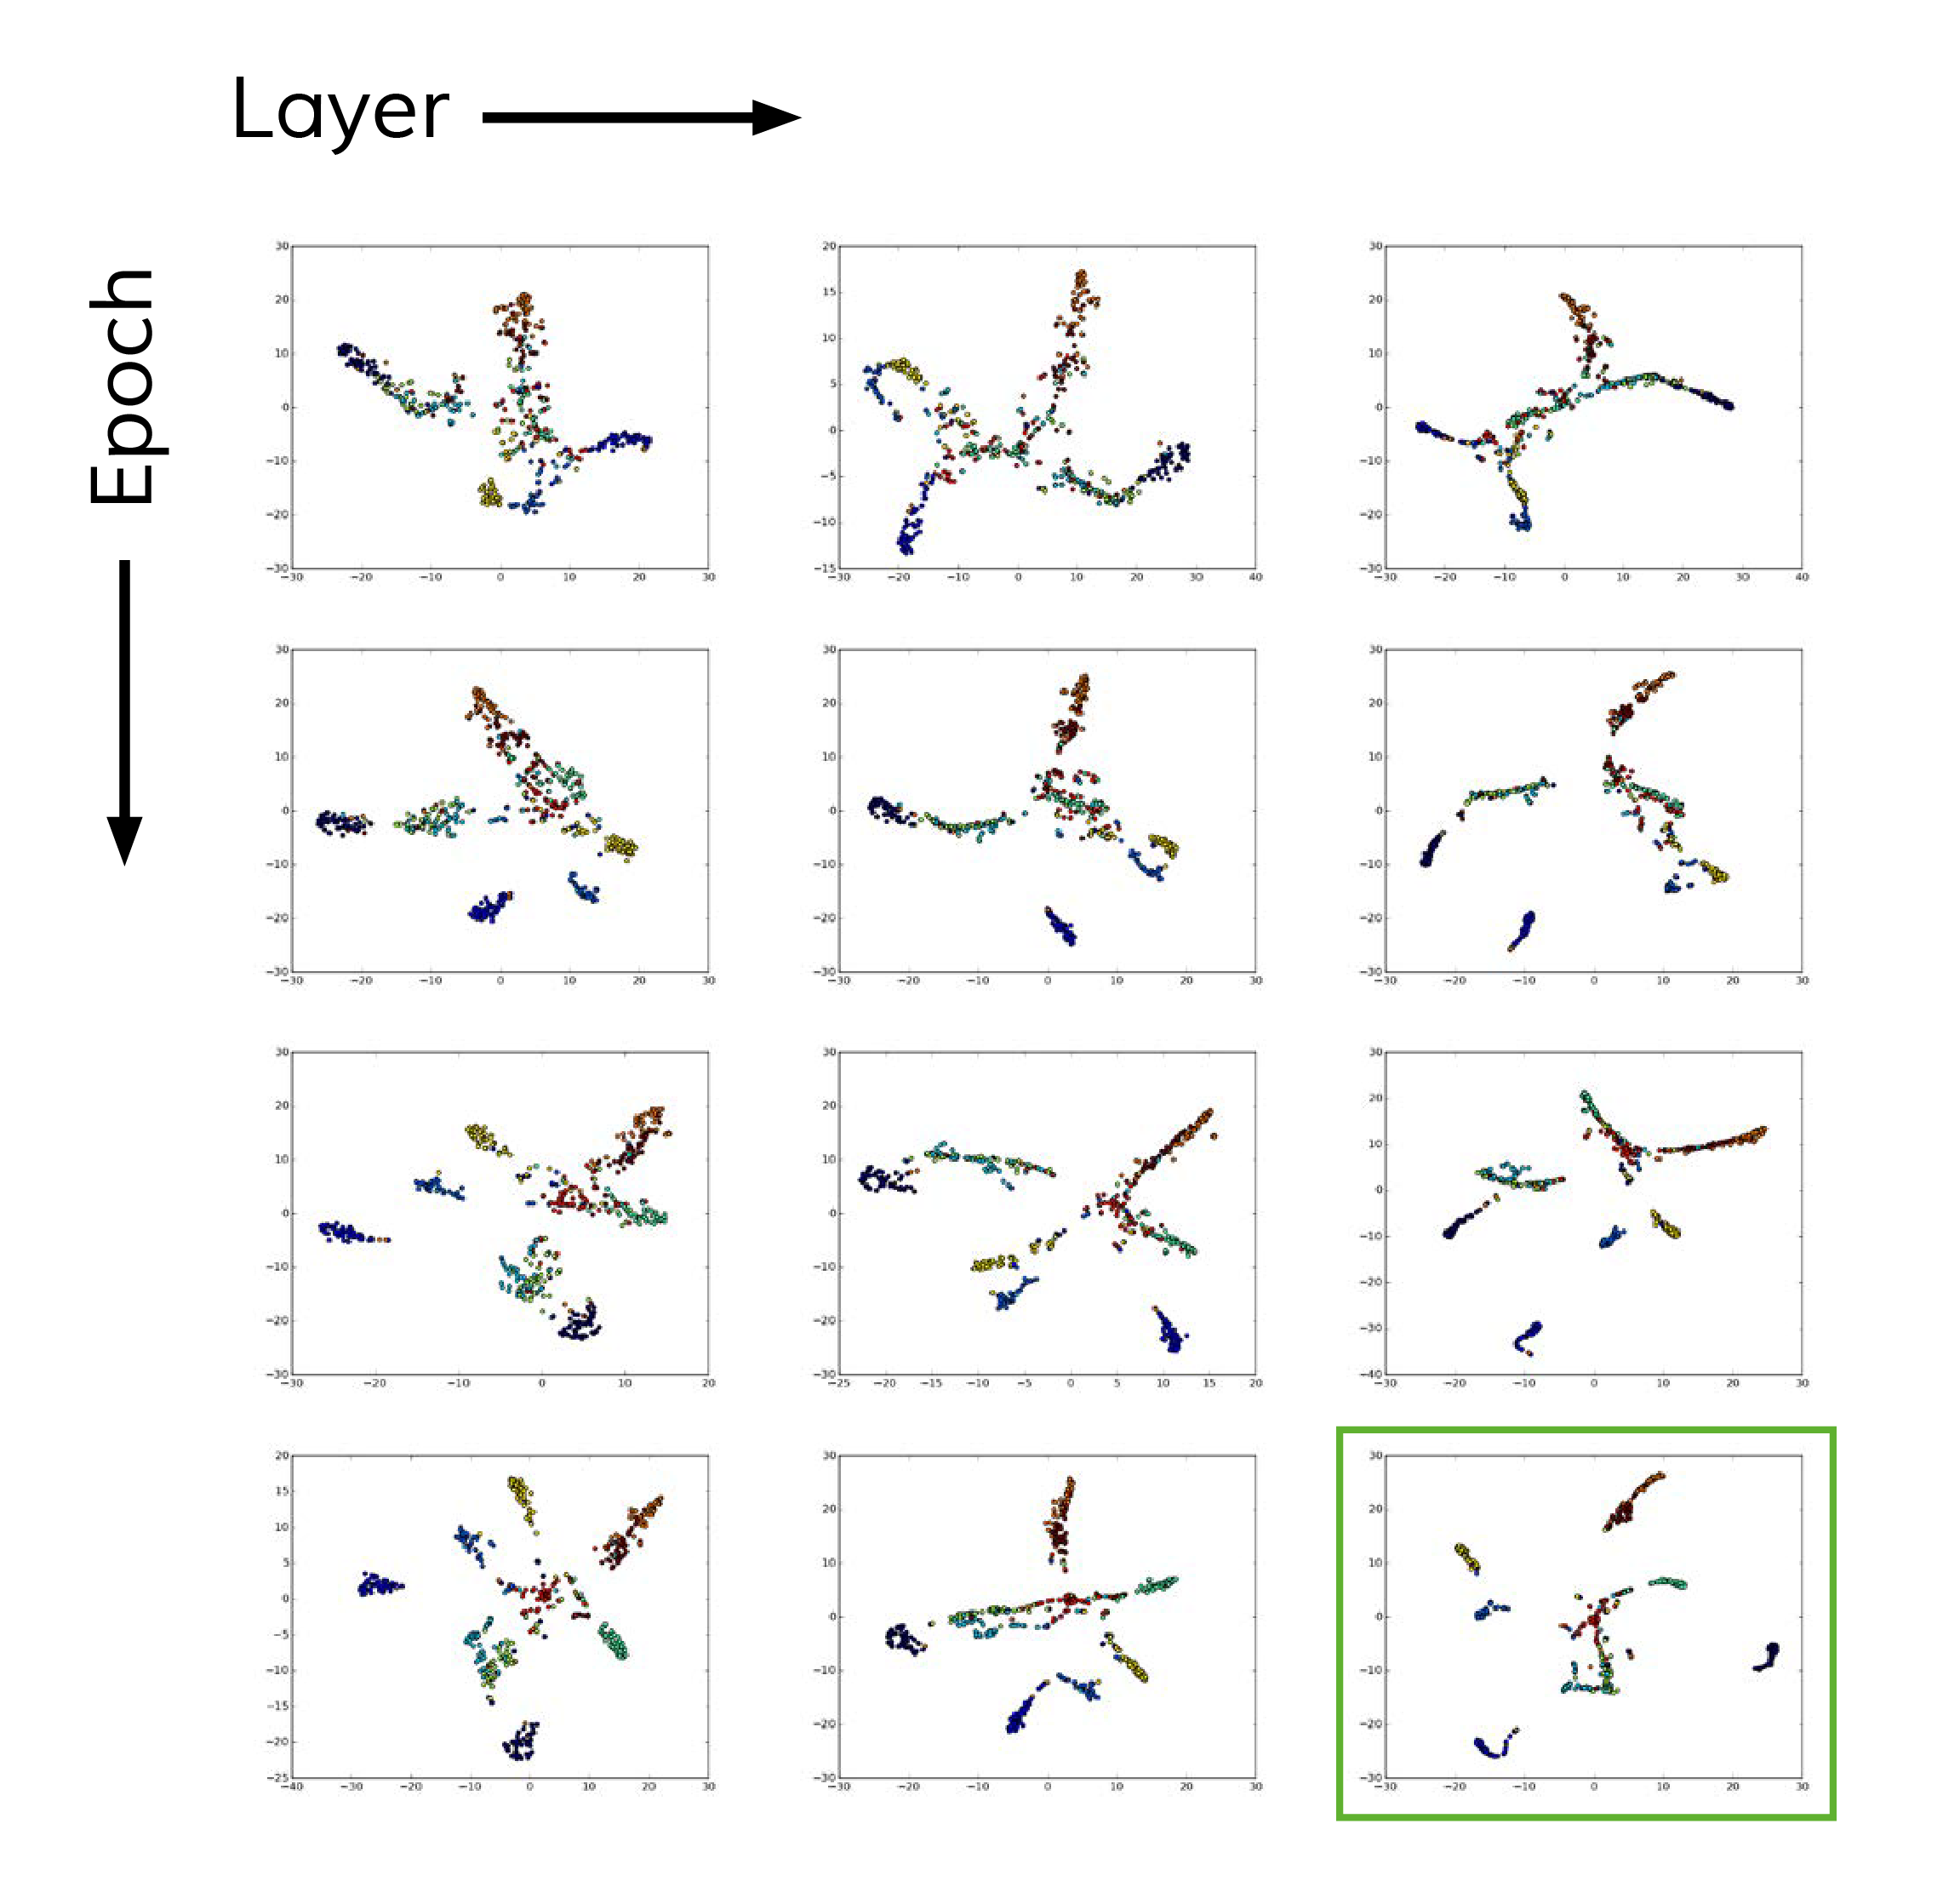
\includegraphics[width=12cm]
    				{img/developing_tsne-01.png} 
    			}}%
    			\caption{Already in the highlighted image it's clear to see the network is learning some distinction between the classes}%
	\end{figure}	
	
	Animating the data enables us to satisfy two more of Tufte's principles:
	\begin{itemize}
		\item Through the animation of tSNE plots across epochs or layers, Edward Tufte's eighth principle to \textit{"encourage the eye to compare different pieces of data"} is now satisfied. The animation naturally encourages the eye to observe differences in the data, as we see the data transform from one shape to another. 
		\item Not only does the animation enable us to compare data, but in doing so we also satisfy Tufte's seventh principle to \textit{augment short term memory through visual patterns}. While it was possible previously to compare tSNE plots by flicking through image - we are essentially automating this process with the animations which, as is often referenced in visualisation theory, leaves an imprint on the retina of the previous image - thus augmenting our memory with the visualisation. 
	\end{itemize}
	
	While animation is definitely a great way to enhance our understanding of the neural network data by bring patterns across the tSNE plots to the fore of our mind, it is not in itself a stand alone too. It is simply a method of processing. 
	\par 
	The aim of this project however is to produce a tool for researchers to use to help them better understand neural networks and tweak parameters to ultimately ensure the successful training of their neural networks.
	\par 
	
	\subsection{Design}
	Before setting out to build the tool, a number of options for the best way to display animations were considered. User interface components were continually sketched, and wire-frames evaluated in response to the needs of neural network researchers and in relation to visualisation best practices. 
	\par 
	Unfortunately it was not possible to get a large range of feedback on the designs due to time constraints, however the little feedback that was attained from fellow students researching with neural networks enabled the project to progress from iterations two, three and four. 
	
	\begin{figure}[H]
    			\centering												{{\includegraphics[width=7cm]
    				{img/SKE-iter1.png} 
    			}}%
    			\caption{An initial sketch displaying animations moving across the screen as the net trains}%
	\end{figure}		
	
	
	
	\subsection{Architecture}
	This early iteration was developed in a lightweight manor in keeping with the \textit{lean product development} methodology \cite{}. This development style states that a \textit{Minimal Viable Product (MVP)} should be built when testing ideas to enable fast testing and learning, which can then be reapplied to the product later without fear of completely rewriting the entire product.
	\par 
		
	\begin{figure}[H]
    			\centering												{{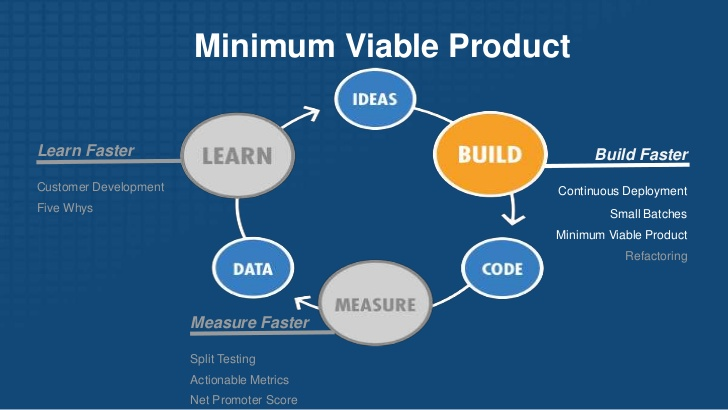
\includegraphics[width=10cm]
    				{img/lean_development.png} 
    			}}%
    			\caption{Lean Development Cycle}%
	\end{figure}	
	
	Here the MVP was a function that could be copied into the researchers neural network and would automatically run after the network had completed training. The implementation extracted the tSNE plot coordinates from the MongoDB database, processed them using pythons \texttt{numpy} into a format that could then be processed with another python library designed for making films, \texttt{MoviePy} \cite{}, which transformed the \texttt{numpy array} of two dimensional tSNE coordinates into a chronologically ordered, by epoch, \texttt{.GIF} animation. These GIF's were saved locally and could be displayed as necessary.
	
	\begin{figure}[H]
    			\centering												{{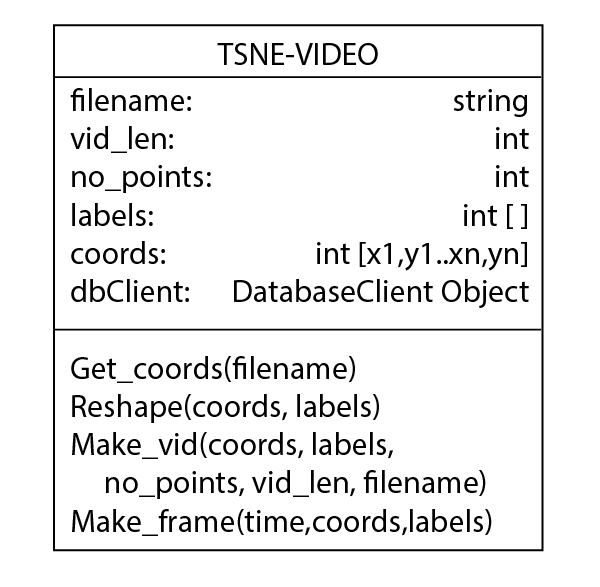
\includegraphics[width=4cm]
    				{img/UML_it1.png} 
    			}}%
    			\caption{Animation Processing}%
	\end{figure}		

	
	\subsection{Evaluation}
	In order to effectively evaluate the success of this product, there are three perspectives that must be addressed: the perspective of the neural network researcher and the insight concerns; the success of the product as a visualisation and the success of the implementation with respect to the previous two goals.
	
	\begin{figure}[H]
    			\centering												{{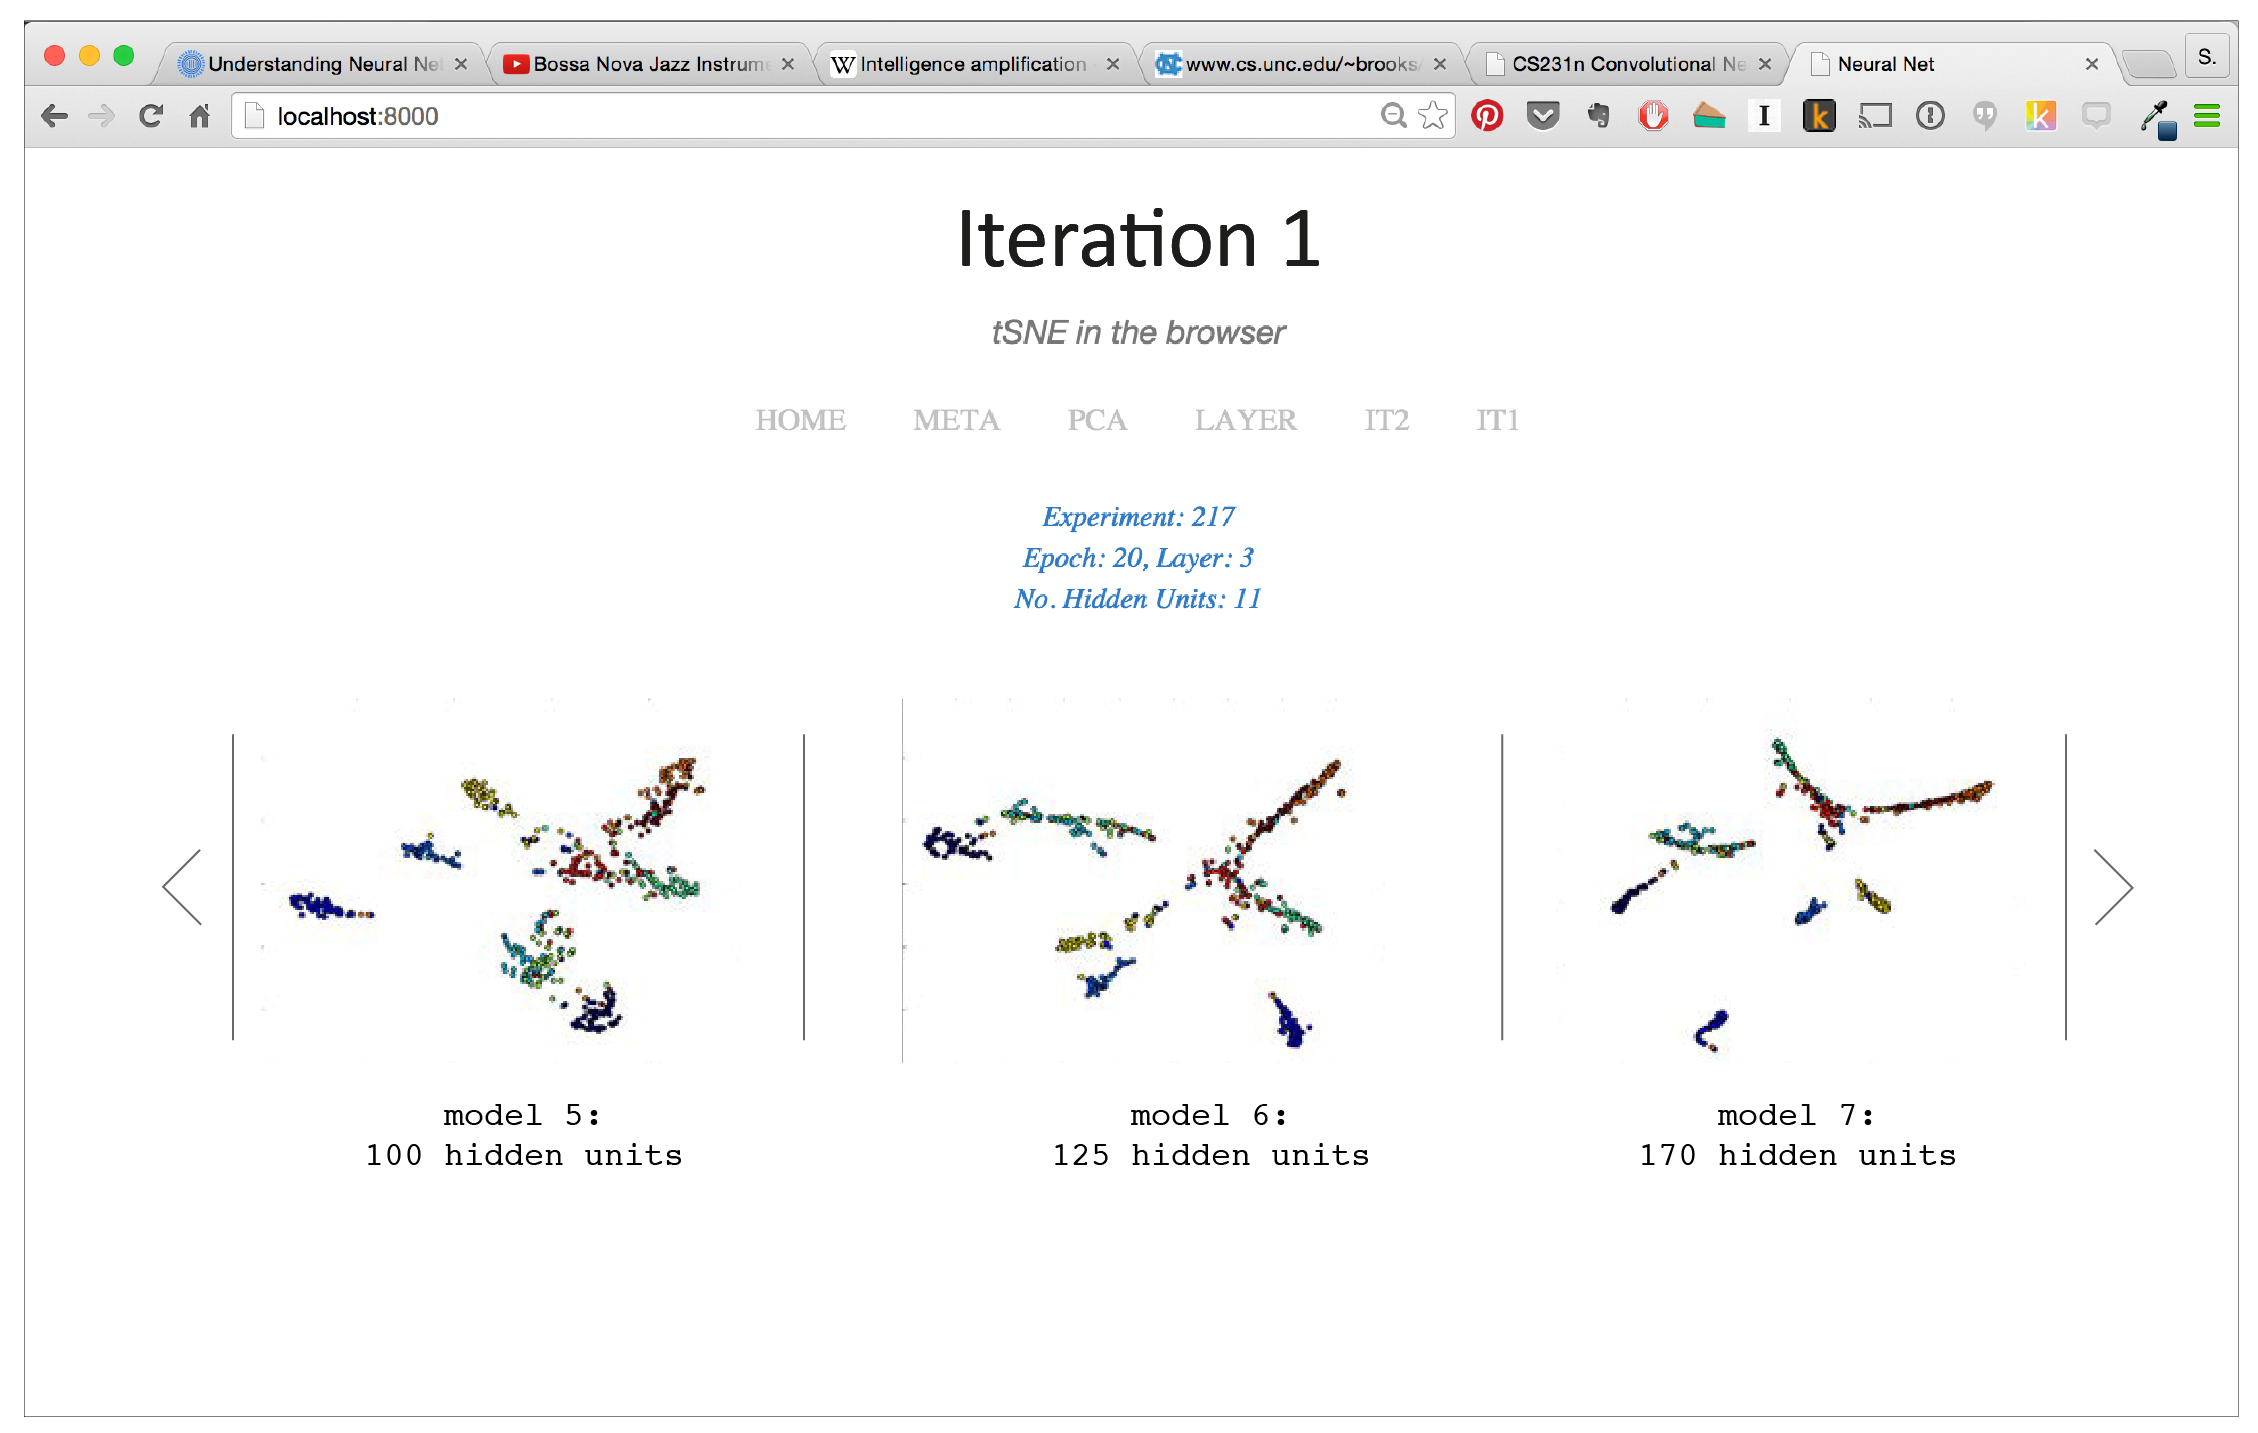
\includegraphics[width=10cm]
    				{img/screenshot_it1-01.png} 
    			}}%
    			\caption{Screenshot iteration 1}%
	\end{figure}		
	
		\subsubsection{Neural Network Perspective}
		The response from a small test sample was fairly clear - while the animations were useful in highlighting that the network changed over time, it was a highly unsatisfactory product for a couple of important reasons: 
		\begin{itemize}
			\item The first and most important consideration was the lack of ability to pause the animations to better understand one abnormal tSNE plot. Now, while this was possible by looking back into the file directory of saved backup plots, this would provide too much friction for any reasonable use.
			\item The second reason, was even if there was the ability to pause, the detail in the plots was limited due to file size constraints - so where a researcher to stop the animation, not much could be learnt.
		\end{itemize}
		
		\subsubsection{Visualisation Perspective}
		From a visualisation standpoint, as assessed in accordance with Tufte's principles, the animations were far more successful than the previous stand alone images.
		\par 
		However, in response to the needs of the neural network researchers the product was deemed to be of too low resolution - and while increasing the resolution was possible, it was decided that the plots should next be created using scalable vector graphics. This would ensure the quality of the visualisation even upon infinite zooming - a useful quality where datasets can have several thousands of points. 
		\subsubsection{Implementation Perspective}	
		As mentioned previously, the implementation was a \textit{rough and ready} solution that could enable a successful iterative process. There was however the realisation that everything should be easily accessible under one package, rather than requiring the user to grapple with lots of moving parts. Again, causing friction to the tool would ensure that it was never used.
		
\clearpage 

\section{Iteration 2 - Online \& interactive}
	\subsection{Introduction}
	In response to the points highlighted by the first design iteration, the second iteration focussed on placing as much of the process online and therefore should enable the much required interactive element of the product. 
	
	\begin{figure}[H]
    			\centering	
    			\subfloat[]								{{\includegraphics[width=0.2\textwidth]
    				{img/Iter2_30_53.png} 
    			}}%
    			\qquad
    			\subfloat[]									{{\includegraphics[width=0.2\textwidth]
    				{img/Iter2_30_59.png}
    			}}%
    			 \qquad
    			\subfloat[]									{{\includegraphics[width=0.2\textwidth]
    				{img/Iter2_31_12.png} 
    			}}%
    			\caption{Screenshots of growth from iteration two}%
    			\label{fig:iter2}
	\end{figure}	
	
	\par 
	It's useful once again to to situate the project in the realm of Edward Tufte's visualisation principles so that we can assess the success of this new proposal that seeks to be interactive and online, and therefore also enabling the use of JavaScript and thus interactivity. In addition to all of the previous Tufte rules that we have successfully achieved, there comes two more by bringing the data online. 
	\begin{itemize}
		\item Through the use of a common interactive concept for the web \textit{tooltips}, which is simply text that hovers above the object that the mouse is focusing upon at any one moment in time, we can satisfy Tufte's sixth principle to \textit{visually highlight your message}. 
		\item In addition, where previously in the animations there was no way to dig into the data without decreasing quality cause by poor pixel representations - the capability of the browser to handle \textit{Scalable Vector Graphics, SVGs} enables the researcher to zoom in on the large data sets to observe the local structure captured by tSNE, and to zoom out observing the global structure. This coincidently allows us to achieve another one of Tufte's principles of quality visualisation" \textit{Reveal the data at several levels of detail}. 
	\end{itemize}
	
	\subsection{Design}
	The previous idea was for the animations to load after each model had trained - displaying the full transformation of a model from one that classified poorly with certain distinct characteristics, to one that classified well - potentially again displaying specific characteristics. 
	\par 
	This version differed in it's approach. Influenced by Andrej Karparthy's tSNE visualisations, this model visualised the optimising of the tSNE cost function over time, or with respect to certain 'steps'. As shown below in the initial sketch designs below the aim was to show how tSNE functioned pulling apart the classes. 
	\par 
	The value of doing this would be to observe how the local and global structures emerged over the course of the tSNE optimisation to a 2D representation that more accurately represented the multiple dimensions of the neural network activation data. 
	\par 
	In addition the researcher should be able to choose from the models already stored in the database by selecting a plot based on simple criteria such as: 
	\begin{itemize}
		\item Experiment: choose from all the experiments run since the visualisation tool was created.
		\item Epoch: choose which epoch you want to run, to be able to compare earlier epochs with later ones - testing if the model was indeed still training even if the Loss values had plateaued - enabling you to see if those last few annoying samples were slowly being better classified. For example the unfortunate event where Google's algorithms identified people with Black skin as monkeys - a severe mistake, and one that caused them significant embarrassment. 
		\item Layer: looking by layer shows activations are indeed propagating from one layer to the next, and serving as a proxy to see that the network is actually adjusting the weights later in the network. It's a common, and sometimes hard to diagnose problem, if weights are not changing sufficiently due to poor network initialisation or some other complication.
	\end{itemize}	 
	
	\begin{figure}[H]
    			\centering	
    			\subfloat[Using Angular.js Repeat with Dropdowns]								{{\includegraphics[width=0.4\textwidth]
    				{img/SKE-iter2-A.png} 
    			}}%
    			\qquad
    			\subfloat[Using Angular.js Sliders]									{{\includegraphics[width=0.4\textwidth]
    				{img/SKE-iter2.png}
    			}}%
    			\caption{ }%
    			\label{fig:iter2}
	\end{figure}		
		
	\subsection{Architecture}
		In order to bring the content online, the author spent a sizeable amount of time learning to use the \textit{MEAN} development stack: Mongo (for the database), Express (for the routing), Angular (for the front-end interaction) and Node (the server). 
	\par 
	In addition, in order to produce the much called for SVG plots the \textit{D3.js}, or \textit{Data Driven Documents} was used. 
	\par 
	Now that the project is entirely written in javascript, it seemed pointless to have a Python system crunching the tSNE data as well. Far better in fact to simply store in the database and call from the JavaScript sever to feed to the front end via. a \textit{RESTful API}. This therefore required a JavaScript implementation of the tSNE algorithm as well. 

	\begin{figure}[H]
    			\centering												{{\includegraphics[width=4cm]
    				{img/UML_it2.png} 
    			}}%
    			\caption{Visualisation}%
	\end{figure}
	
		\subsubsection{tSNE.js}
		Andrej Karpathy, a Stanford PhD student researching neural networks has developed a series of JavaScript based projects that relate to neural networks. While his famous projects is a implementation of a convolutional neural network, he also openly supplies an implementation of the tSNE algorithm in JavaScript - \texttt{tSNE.js}.
		\par 
		This second iteration used tSNE.js and followed the example given by Karpathy online in order to produce a tSNE plot that grows over time. The graph below is his implementation applied to word-embeddings \cite{karpathy} 
		
	\begin{figure}[H]
    			\centering												{{\includegraphics[width=7cm]
    				{img/karpahy_tsne.png} 
    			}}%
    			\caption{Andrej Karpathy Implementation}%
	\end{figure}	
		
	\subsubsection{Node Server}
		Node.js is a platform built on Chrome's JavaScript runtime for easily building fast, scalable network applications. Node.js uses an event-driven, non-blocking I/O model that makes it lightweight and efficient, perfect for data-intensive real-time applications that run across distributed devices.\cite{Dahl2009}
		\par 
		In 2011, a package manager was introduced for Node.js library, called \textit{npm}. The package manager allows publishing and sharing of open-source Node.js libraries by the community, and simplifies installation, updating and un-installation of libraries \cite{Dahl2009}.
		\par 
		These features make Node.js an ideal option for developing a visualisation tool for, and were it developed further could lead to the easy development of a version for node package manager. Indeed, npm is already a common method of sharing proprietary DNN software within the deep learning community.
		 
		\subsubsection{D3 Visualisation Library}
		D3.js, or Data Driven Documents, is a JavaScript library for producing dynamic, interactive data visualizations in web browsers.
		\par 
		D3 allows the binding of arbitrary data to a Document Object Model (DOM), and then apply data-driven transformations to the document. For example, you can use D3 to generate an HTML table from an array of numbers. Or, use the same data to create an interactive SVG bar chart with smooth transitions and interaction.\cite{Bostock2011a}.
		\par
		D3 is extremely fast at supporting large datasets, making it ideal for working with the large output of the neural networks. The dynamic behaviours enabled for interaction and animation make it highly suited to the task of exploring visualised data with the aim of deriving new insights from such data.

	D3 uses a sophisticated method of joining data with the DOM. With three simple commands (Enter, Update, Exit) it enables you to tell D3 the relationship you want to exist between your data and your SVG. For example, you might want circle elements to correspond to data. Instead of telling D3 to create circles and then collect all the circles and assign each data point a circle, as you might do with jQuery.
	
	\begin{figure}[H]
    			\centering												{{\includegraphics[width=7cm]
    				{img/d3enterupdateexit.png} 
    			}}%
    			\caption{D3 Data Binding}%
	\end{figure}	
	
	Data points, such as the coordinates in a tSNE plot, that are joined to existing circles produce the update selection. While unbound data (data for which there are no circles) produce the enter selection (left). Then, any remaining unbound circles produce the exit selection (right). Often these are the points we want to remove. The significance of this is that a scatter plot can be created with not much more code that the following code:
	
	\begin{figure}[H]
    			\centering												{{\includegraphics[width=7cm]
    				{img/d3codeenterupdateexit.png} 
    			}}%
    			\caption{D3 managing data responsively}%
	\end{figure}	
	
	The simplicity of the D3 library is what makes it so powerful, and it was chosen in this project for that reason. Ideally with an implementation started in d3.js, other researchers can build upon the software with relative ease to continue to create powerful tools. 
	\par 
	D3 is not just a great way of creating the scalable vector graphics that we require to enable researchers to look both at the global and local structure of the tSNE plots, but also allows us, with relative ease, to bring more detail to the plots. Coding in text tooltips for example ensure that we meet Tufte's principle on focusing in on detail. 
	\par 
	The following images show the tooltips used in the second iteration of the project and the relative ease at which they can be encoded.
	
	\begin{figure}[H]
    			\centering	
    			\subfloat[Text-tooltips]								{{\includegraphics[width=0.4\textwidth]
    				{img/tooltip-text-iter2.png} 
    			}}%
    			\qquad
    			\subfloat[Easily adaptabel Tooltip d3.js Code]									{{\includegraphics[width=0.4\textwidth]
    				{img/tooltip_code.png}
    			}}%
    			\caption{ }%
    			\label{fig:iter2}
	\end{figure}	


	\subsection{Evaluation}
	In order to retain some consistency, the evaluation methods were retained the same. Assessing the quality of the product under the three main categories of neural network research usefulness, visualisation quality and implementation quality.
	\par 
	This is a screen shot of the complete second iteration once the cost function has been optimised and the image zoomed in upon. It demonstrate the high-fidelity of the d3.js SVG graphic, and shows a marked improvement upon the low fidelity pixelated animations.

	\begin{figure}[H]
    			\centering												{{\includegraphics[width=10cm]
    				{img/Iter2_31_28-01.png} 
    			}}%
    			\caption{Zoomed in screenshot}%
	\end{figure}
	
	Below are a number of screen shots depicting the final product during the stages of tSNE optimisation over it's cost function given at epoch 20,  Layer 3 for a derivation of the Hinton network but with only 11 Hidden ReLU units in each layer.
	
		
		\subsubsection{Neural Network Perspective}
		It was widely agreed that this implementation was far superior to the GIF animations. The ability to zoom and interrogate data at different scales was welcomed, and the retention of quality in doing so was also a marked improvement. Also notably the simple use of tooltips to display the actual value of the data, rather than just using colour, was a great addition as it allowed a user to first zoom in on some unlikely data samples and then see which exact data samples were causing the problem.
		\par 
		While the product was deemed to be a marked improvement on the previous iteration, there were still an number of changes that clearly needed to be made:
		\par 
		The version was criticised for taking too long in the processing of each tSNE plot. This makes it hard for users to flick between layers or epochs in order to start identifying patterns - and violates Edwards Tufte's seventh principle that visualisation should augment short term memory through visual patterns. Here, the patterns emerged too slowly and providing an ineffective means of comparison. The slow result is likely due to the slow performance of the client side optimising of the tSNE function used. 
		\par 
		While the tooltips provided a useful way of understanding which points corresponded to which output classification in the range of one to nine, they were ineffective in demonstrating exactly which input values were causing this error. This is something that was addressed in version three.
		
		\subsubsection{Visualisation Perspective}
		While in the neural network criticism above it's clear to see that there are a number of visualisation improvements that needed to be addressed, there were significant visualisation discoveries made for the authors perspective. Most notably was the use of \textit{D3.js} transitions to smooth over the difference between each step in the iterative refinement of the tSNE plot. These transitions are often used for the 'WOW' factor, however in this instance they provide an important functional use, and allow the eye to easily follow specific points trajectories in space. This is useful in allowing the user to observe anomalies or peculiar changes in the data over time.	
		\par 
		The introduction of transitions here is significant, and should be used in all future versions to enable easier pattern spotting within the changing data sets, be this between model, epoch or layer.
	

\clearpage 
				
\section{Iteration 3 - Epochs \& Layers}
	\subsection{Introduction}
	There were a number of issues that needed to be addressed in response to the feedback from the previous iteration, and also upon considering the implementation there were some blatant improvements that could quickly be made that could help streamline the project as a whole. 
	\par 
	Where the previous iteration focussed on the tSNE optimisation of a single activation output from a specific model, epoch and layer, the new construction would select a model and demo pre-calculated tSNE plots  with a user interface that enables the researcher to quickly analyse the differences between layers visually.
	\par 
	This allows researchers to answer a number of questions very rapidly, observing changes across layers demonstrates if the back-propagation algorithm is successfully penetrating all layers and producing transformations in the weight layers. Observing changes across epoch demonstrates whether these layers are learning over time, or if they are simply arbitrary mapping the data. 
	\par 
		
	\begin{figure}[H]
    			\centering												{{\includegraphics[width=10cm]
    				{img/sne_plot_E2_l1.png} 
    			}}%
    			\caption{Epoch 2, Layer 1 from different models}%
	\end{figure}	
	
	In addition being able to hover over the points in the D3.js plot to show the tooltip of specific numbers allows the researcher to follow which numbers are being confused with which others - indicating that perhaps in their training set they should include more rotated sevens to allow the network to properly distinguish them from nines. 
	\par 
	In essence, by plotting the graphs across the epochs and layers within one experiment there is a vast amount of information that can be gleaned from these plots.
	
	\subsection{Design}	
	There were a number of important design considerations for this iteration. This fell primarily into two parts; control and display.
	\par 
	Once users had chosen their model, there needed to be an user interface element that would allow researchers to quickly change from one epoch or layer to the next. A number of different methods were tried using Angular.js including sliders, check-boxes and drop down menus. However while these all failed to unify the transition that was occurring, by which I mean they failed to highlight where exactly a layer-epoch combination sit with respect to any other layer-epoch combination. 
	\par 
	Coincidentally the best method found was to use another d3.js implemented scatter plot that would show exactly all the points that had been plotted, and so a researcher could quickly get an overview of the data as well as switch between different layer-epoch combinations simply by moving the mouse. 
	\par 
	This allows users to see exactly how far along the progression for that particular model changed, and the events leading up to this - be them at an epoch or layer scale.  

	\begin{figure}[H]
    			\centering												{{\includegraphics[width=7cm]
    				{img/SKE-iter3-C.png} 
    			}}%
    			\caption{Wireframe Design}%
	\end{figure}	
	
	In addition to the control block was the display; the section where the actual tSNE, or by this point Barnes Hut SNE (a faster version), was plotted. This section is the real information that reveals the insights, and the transitions from layer to epoch became exactly that - d3.js transitions. 
	\par 
	D3.js has a useful ability to transition from one representation of a data point (or datum) to another via a number of rendered transition states. This allows the human eye to follow how specific points move with ease, and enables us to re-enact more of Tufte's guiding visualisation principles to \textit{augment short-term memory loss with visual patterns} - here the transitions literally allow us to follow specific data points as they move across the screen.
	\par 

	
		\begin{figure}[H]
    			\centering	
    			\subfloat[Barnes Hut SNE after applying to the imagified scatterplots]								{{\includegraphics[width=0.3\textwidth]
    				{img/d3Transitions.png} 
    			}}%
    			\qquad
    			\subfloat[Barnes Hut SNE after applying Principle Components Analysis]									{{\includegraphics[width=0.4\textwidth]
    				{img/SKE-iter3-D.png} 
    			}}%
    			\caption{}%
    			\label{fig:epoch_layer}
	\end{figure}
	
	Another important element to notice in comparison to the initial iteration where essentially static images were used, is that here when the image is no longer static the axis are no longer relevant.
	\par 
	It's possible to argue that axis were never relevant due to the lack of units, but they did represent differing degrees of spatial distribution. Here it's important the all of the images are presented in the same axis across the data so that patterns can be more easily spotted. 
	\par 
	D3.js has yet another very useful tool \texttt{d3.scale.linear} which essentially normalises the data within the visual range on the screen. Mapping the input domain to the output range, and thus fitting the data.
	\begin{figure}[H]
    			\centering												{{\includegraphics[width=7cm]
    				{img/d3scales.png} 
    			}}%
    			\caption{d3 scaling elements}%
	\end{figure}	
		
	\subsection{Architecture}
	
	\subsubsection{Entirely Python}
	Iteration one was implemented in a lightweight way with relatively little RESTful API use. Iteration two performed the interaction using a Node.js server to keep the entire toolkit in JavaScript - supposedly ensuring the neatness of the project. 
	\par 
	In iteration three however, the node.js and express.js back-end components were replaced with a python \textit{Flask} which is a \textit{Sinatra-like} micro web application framework written entirely in Python for the use in major web applications. The framework is used by companies such as Pinterest and LinkedIn and serves as a far more appropriate product for the back-end in this project as well.
	\par 
	The entire architecture has now been streamlined with Python entirely in the back end; from the neural network, to the database, to the RESTful server and post-processing functionality. The entire front end is JavaScript using Angular.js for basic manipulation of the DOM and d3.js for the interactive visualisations.
	\par 
	
	\subsubsection{Streamlined Database}
	In addition to the restructuring of the architecture to have a clearer divide between back-end Python and front-end JavaScript - the Mongo database is now interacted with using a python toolkit \texttt{PyMongo}. 
	\par 
	This opportunity allowed a streamlining of the database structure as well, from the model represented in the ER schema at the beginning of the report to the following, perhaps slightly clumsier, however far easier to interact with JSON storage format.
	\par 
	This new database schema stores the most important parameters for understanding the neural network, as well as the key data required for the visualisations.
	

	\begin{figure}[H]
    			\centering												{{\includegraphics[width=4cm]
    				{img/UML_data.png} 
    			}}%
    			\caption{PyMongo Interaction}%
	\end{figure}		
	
	\textbf{TODO}: adjust this to fit this third iteration, the fourth iteration is where the PCA and META SNE come in.
	
	\begin{figure}[H]
    			\centering												{{\includegraphics[width=9cm]
    				{img/actual_json.png} 
    			}}%
    			\caption{Final Simplified JSON scheme for PyMongo}%
	\end{figure}
	
	\subsubsection{Tooltip Adaptation}
	Another small change made, was to highlight the text tooltips by adding a fill to the background enabling the text to pop out - where previously the numbers where occasionally obscured.
	\par 
	
	\begin{figure}[H]
    			\centering												{{\includegraphics[width=5cm]
    				{img/tooltip-text-iter3.png} 
    			}}%
    			\caption{Tooltips}%
	\end{figure}	
	
	In addition to enhancing the text tooltip visibility, it was felt that a higher fidelity approach which allowed one to explore not just the classification of points better, but to understand which input pieces of data these represented. 
	\par 
	Initially the attempt involved trying a number of options uploading the \texttt{.png} images of the MNIST dataset to be rendered each time the user hovered over a point. This however was slow and contrasted to the tight approach of the d3.js application. 
	
	\begin{figure}[H]
    			\centering												{{\includegraphics[width=5cm]
    				{img/tooltip-image-iter3.png} 
    			}}%
    			\caption{Tooltips}%
	\end{figure}	
	
	\par 
	After some unsatisfactory attempts and exploration of other methods, the method used in the Chris Olah blog post \cite{Olah2014d} was discovered. It took a substantial amount of time to work out how the implementation worked, however it simply used the same \texttt{base64} arrays that had been used previously to store the MNIST dataset in the Mongo database. 
	\par 
	Olahs method used the \textit{HTML5 Canvas} to render the points in the browser after uploading the entire dataset in one long \textit{base64} array. The length of the input (784 pixels) was used to index the array and render it live using a combination of d3.js and HTML5 canvas.
	\par 
	While it was possible to utilise some of my previous implementation alongside Olahs, it was decided to simply adapt the version produced by Olah and build upon it to save time and not \textit{reinvent the wheel}.	
	\par 
	In addition to these changes a number of other changes were required in the implementation of connecting to the RESTful API, and an interaction class was built that should ensure the easy adaptation for different purposes by researchers with different goals to those used in this project.
	
	\subsection{Evaluation}
	Below are two final screen shots from this third iteration of the product. 
	
	
	\begin{figure}[H]
    			\centering	
    			\subfloat[]								{{\includegraphics[width=0.45\textwidth]
    				{img/layer_epoch.png} 
    			}}%
    			\qquad
    			\subfloat[]									{{\includegraphics[width=0.45\textwidth]
    				{img/layer_epoch2.png} 
    			}}%

    			\caption{}%
    			\label{fig:pca_varimax}
	\end{figure}
	
	
		\subsubsection{Neural Network Response}
		There are several advantage of this method in comparison to the previous. Where the previous helped users understand the how the data is clustered using the tSNE algorithm, this new method is a vast improvement in analysing the data for the purpose of understanding what these networks are doing.
		\par 
		The ability for researchers to quickly compare changes across epoch allows them to identify data-points that are constantly failing to be captured. This representations created are demonstrated in the tSNE plots, and those that cluster more effectively are the networks that
		\par 
		The d3.js transitions that were used previously to highlight the changes between iterations in the optimisation of the tSNE cost function. Here however the transitions were used to enable the viewer to observe the translation of a data point from one position to another within the tSNE visualisation of the network representation at a given layer and epoch in a specific model.
		\par 
		After observing however that several of the tSNE plots appeared to simply be rotations of one another it was questioned whether researchers would accurately be able to diagnose which changes were the neural network actually learning, and which were simply transformations of the space in which no benefit actually occurs. For this reason, suggested improvements would be ensure that it was possible to identify which of the tSNE representations of the data were transformations of one another.
		\subsubsection{Visualisation Response}
		The key visual changes here were the introduction of transitions between layers and epochs enabling the user to observe patterns more accurately, and in addition ensuring that Edward Tufte's guide was still being followed.
		\par 
		The other major change was the introduction of the image tooltip. Previously the text-tooltip enabled the researcher to view the classification result to the accuracy of the output layer, however here each data point directly corresponds to one of the input values, each of which is visually rendered in the browser. This adaptation of Chris Olahs blog post provides a much needed fidelity within the project.		
	\subsubsection{Implementation Response}
	There were a number of significant implementation changes in iteration three; a more streamlined database, a properly separated Python back-end and JavaScript front-end, and the introduction of an adapted version of Chris Olahs \cite{Olah2014c} d3.js code that includes the image tool-tips.
	
	\begin{figure}[H]
    			\centering												{{\includegraphics[width=14cm]
    				{img/UML_d3.png} 
    			}}%
    			\caption{Adapted \& Extended Olah D3.js interaction}%
	\end{figure}	
	
	\par 
	The streamlined database ensures that researchers can easily interact with the product. The distinctive front and back-ends ensures that they can be used independently of one another. And the adapted and improved visualisation infrastructure ensures that it is easier for researchers to interact with.
	
	\clearpage 
	
\section{Iteration 4: metaSNE \& Principle Component Analysis}
	
	\subsection{Introduction}
	While the previous iteration was a fairly successful implementation as it allowed researchers to actually observe at both a fine grain detail of misclassified data points as well as providing an overview of the experiment as a whole by enabling the researcher to browse by epoch and layer, the challenge of identifying changes because of rotational data was problematic.
	\par 
	The main focus in this section is the exploration of principle component analysis as a method for enabling the researcher to perceive rotational data more clearly. 
	\par 
	However this process can be quite mathematically complex, and can be approximated instead by using a combination of Principle Component Analysis (PCA) and Varimax Rotation to orthogonalise the data. 	
	\par 

	\subsubsection{Isometries in Representations}
	Many datasets have rotational duplicates appearing across them, and in data science \& mathematics this is a common problem. Where a representation contains a transformations in the \textit{Euclidean} space, these transformations are often called \textit{Isometries} and are transformations such as rotation or flipping. 
	\par 
	In the tSNE plots that visualise the representations being formed by the neural networks it's important to distinguish which plots demonstrate new pieces of information being learnt, or are they simply just translations across the Euclidean space - where by nothing really has been learnt.
	\par 
	In his blog post on \textit{Representations} \cite{Olah2014} explores this notion of isometries stating that for any representation $ X $ there is an associated metric function, $ d_{x} $, which gives us the distance between pairs of points within that representation. For another representation $ Y $, $ d_{x} = d_{y} $ if and only if $ X $ is isometric to $ Y $. This is exactly the form with removal of isometries required.
		\par 
		The issue with $ d_{x} $ however is that it is a function on a very high-dimensional continuous space, caused by the need to consider the distance between functions as infinite dimension vectors.
		 
		$$
		D_X = \left[\begin{array}{cccc} 
		  d_X(x_0, x_0) & d_X(x_1, x_0) & d_X(x_2, x_0) & ... \\
		  d_X(x_0, x_1) & d_X(x_1, x_1) & d_X(x_2, x_1) & ... \\
		  d_X(x_0, x_2) & d_X(x_1, x_2) & d_X(x_2, x_2) & ... \\
		  ... & ... & ... & ... \\ 
		\end{array} \right]
		$$
		
		This transformation into metric space can be incredibly complex, so the approach taken instead approximates the method above by using \textit{Principle Component Analysis} and \textit{Varimax Rotation} to orthogonalise the PCA mappings.
		
		\begin{figure}[H]
    			\centering												{{\includegraphics[width=0.4\textwidth]
    				{img/sne_plot_E2_L1_rotation.png} 
    			}}%
    			\qquad
    			{{\includegraphics[width=0.4\textwidth]
    				{img/sne_plot_E2_L3_rotation.png} 
    			}}%
    			\caption{Experiment where between two layers the data has essentially just been flipped - demonstrating nothing particularly new has been learnt}%
		\end{figure}

	\subsection{Design}
	The fourth iteration of this project is where the development ends. There are still improvements that can be made which can be made, and will be discussed in the concluding section, however by this point there is certainly a tool that can be utilised to make important decisions. 
	\par 
	There are five key components to this final selection that is hopefully incredibly straightforward to use:
	\begin{itemize}
		\item First, the neural networks themselves: two neural networks are provided with the tool, a convolutional network and a feed forward network as described in the introduction. These two classes are easily adaptable under the \textit{Lasagne} guidelines.
		\item Second, the saving functionality afforded by \textit{PyMongo} and the \textit{MongoDB} database that saves key data in an easily accessible format to a local database.
		\item Third, the post-processing functionality that provides the PCA / meta-SNE plotting explained in this chapter. 
		\item Fourth, the RESTful API providing data to the client.
		\item Fifth, the front end \textit{Angular.js} and \textit{D3.js} application consisting of an easy to use homepage where the user can select the model they want to explore, and the visualisation pages where the user can interrogate their data.
	\end{itemize}
	
	Below are two sketch diagrams that demonstrate the simplicity of the front end.
	
		\begin{figure}[H]
    			\centering	
    			\subfloat[Homepage]								{{\includegraphics[width=0.4\textwidth]
    				{img/SKE-iter3-E.png} 
    			}}%
    			\qquad
    			\subfloat[PCA interaction]									{{\includegraphics[width=0.4\textwidth]
    				{img/SKE-iter3-B.png} 
    			}}%
    			\caption{}%
    			\label{fig:pca_varimax}
	\end{figure}
	
	\subsection{Architecture}
	The final architecture has a number of components as were described in the previous design section; however the addition of the Principle Component Analysis post-processing is explored below. 
	\par 
	
	\subsubsection{PCA Post-Processing}
	In order to determine which techniques worked, or did not work, for better displaying those plots that were isometries of one another - or were very similar under a number of mathematical criteria - the following experiment was undertaken that compared three alternative approaches upon a test set that could prove the success or failure of each of the methods.
	\par 
		
	\begin{figure}[H]
    			\centering												{{\includegraphics[width=7cm]
    				{img/rotatedDataOriginal.png} 
    			}}%
    			\caption{The test dataset}%
	\end{figure}	
	
	The test set, above, was a number of uniformly generated $x$ and $y$ points that when plotted produced a dataset that consisted of two identical triangles that had been rotated by differing amounts, and three identical squares that had likewise been rotated by differing degrees with differing offsets.
	\par 
	The three different approaches were used in an attempt to generate an effective \textit{metaSNE} plot, such that plots which were most similar when disallowing isometry data to influence difference. The following methods tested were as follows:
	\\\
	\\\
	\textbf{Image Compression}
	\par
	The first method took influence from the tSNE plots of the MNIST dataset where each of the 28 pixel by 28 pixel images were had their dimensions collapsed into a single 784 pixel array before the tSNE algorithm is implemented upon it.
	\par 
	With the scatter plots, in order to do this, the (x, y) coordinates needed to first be transformed into an image with discrete dimensions. For example, a 500 pixel by 500 pixel image. 
	\par 
	There were a number of different methods that could have been employed in order to do this, however the method adopted was to create a two dimensional histogram that were a point to appear within a given coordinate bin, then that bin would be assigned the average of all points situated within it. 
	\par 
	\begin{figure}[H]
    			\centering												{{\includegraphics[width=12cm]
    				{img/2d_historgram_tsne.png} 
    			}}%
    			\caption{Imagifying Scatterplots}%
	\end{figure}	
	
	As can be seen from the figure above this works for the most part due to the relatively high-fidelity of the selected dimensions. However, where two or three points are situated very close together - such as can be seen once or twice below - the transformation taking an average distorts the dataset somewhat. 
\\\
\\\
	\textbf{Principle Component Analysis}
	\par
	The second method attempted was to first apply a Principle Component Analysis, PCA, transformation to the scatter plot in an attempt to remove the majority of the rotational differences. 
	\par 
	PCA is a statistical procedure that converts the set of points along a number of principle components. The largest principle component has the largest possible variability in the data, and each succeeding component has the highest variance possible under the constraint of those preceding it.
	\par 
	This mapping of plots along it's principle components should remove the majority of rotational data held within the plots, and clearly works as is demonstrated in the plot below on the left.
	\par 
	This second method was far more successful than the first in accurately distinguishing the differences and similarities in the original dataset once plotted, however upon application of tSNE the points were indistinguishably plotted.
	\\\
		\begin{figure}[H]
    			\centering	
    			\subfloat[Application of Principle Component Analysis]							{{\includegraphics[width=0.3\textwidth]
    				{img/PCArotations.png} 
    			}}%
    			\qquad
    			\subfloat[Application of Varimax Orthogonalisation]									{{\includegraphics[width=0.3\textwidth]
    				{img/VarimaxRotations.png} 
    			}}%
    			\caption{}%
    			\label{fig:varimax}
	\end{figure}

	\textbf{PCA \& Varimax Rotation}
	\par
	After the unsatisfactory results produced by the PCA process, it was decided that the datasets needed to be simpler for the tSNE algorithm to calculate. 
	\par 
	After much searching, a solution presented itself in the form of \textit{Varimax Rotation} \cite{Lin2012} which orthogonalises the data such that the actual coordinate system is unchanged, but the orthogonal basis that is being rotated is aligned with those coordinates. This produced the plot on the right which aligned the test set perfectly into it's original triangles and square being centred directly on top of one another - thus removing the isometric data we wanted to remove.
	\par 
	The plot below demonstrates on the left the Barnes Hut SNE output when applied simply to the PCA rotated data, and the plot on the left after the data has occurred the Varimax Rotation as well - the former fails to accurately represent any of the data as similar, but rotations of one another, while the latter does exactly as desired - separating the squares from the triangles, and demonstrating that they are simply slight variations of one another.

	\begin{figure}[H]
    			\centering	
    			\subfloat[Barnes Hut SNE after applying Principle Components Analysis]									{{\includegraphics[width=0.23\textwidth]
    				{img/BHafterPCAOnly.png} 
    			}}%
    			 \qquad
    			\subfloat[Barnes Hut SNE after applying Principle Components Analysis, and Varimax Orthogonalisation]									{{\includegraphics[width=0.23\textwidth]
    				{img/BHrotations.png} 
    			}}%
    			\caption{}%
    			\label{fig:pca_varimax}
	\end{figure}


	It is this final version: PCA and Varimax Rotation that is used in the final tool to enable researchers to get a better grasp upon how similar these scatter plot really are.
	
	\begin{figure}[H]
    			\centering												{{\includegraphics[width=7cm]
    				{img/UML_plot.png} 
    			}}%
    			\caption{Post-Processing}%
	\end{figure}	
	
	
	\subsubsection{A tool for visualising neural networks}
	The final architecture for the project remains very similar to that of the previous iteration. 
	\par 
	The	diagram below explains the interconnection between the various parts:
	\begin{itemize}
		\item \textbf{Client Side}
			\par 
			Three components:
			\begin{itemize}
				\item The network experiment selection, and visualisation selection
				\item The browse by animation section
				\item The interactive section where the researcher can explore by Epoch, Layer, PCA/Varimax centred, or pure meta-SNE (tSNE applied directly to tSNE).
			\end{itemize}
		\item \textbf{RESTful API}	
			\par 
			The Flask Restful API enables the information on the server side to remain hidden until needed. It also ensures the site can load quickly without having to upload vast amounts of neural network data. 
		\item \textbf{Server Side}
			The server side has two primary components: the database and the neural network processing elements. The neural network processing however is split into a further three parts:
			\begin{itemize}
				\item The Neural Networks themselves which can be called from the network automation section.
				\item The helper functions which facilitate the extraction of data from the neural network and store it appropriately
				\item The post-processing unit which extracts from the database all stored tSNE plots, and processes them to produce a meta-SNE plot and PCA/Varimax plots.
			\end{itemize}
	\end{itemize}
	
	\begin{figure}[H]
    			\centering												{{\includegraphics[width=7cm]
    				{img/UML_server.png} 
    			}}%
    			\caption{Basic RESTful interaction}%
	\end{figure}	
	
	\begin{figure}[H]
    			\centering												{{\includegraphics[width=10cm]
    				{img/Flow_diagram-01.png} 
    			}}%
    			\caption{The architecture behind the whole system}%
	\end{figure}	
				
				
	\begin{figure}[H]
    			\centering												{{\includegraphics[width=14cm]
    				{img/all_combined-01.png} 
    			}}%
    			\caption{UML, ER, Scheme diagram hybrid}%
	\end{figure}	

	
\subsection{Evaluation}
These two final screen shots demonstrate the control cluster side by side with the display cluster. The control has been created using the PCA/Varimax combinations such that points next to one another are similar or may be rotations of one another. The display shows the tSNE data once it has been transformed along the principle components and orthogonalised with Varimax. 
\par 
The homepage is a simple place where the researcher can select a model from the database, which will then be passed up to the client side application and the researcher can browse by either: Epoch \& Layer tSNE, PCA \& Varimax tSNE, or, tSNE tSNE (meta-SNE).


	\begin{figure}[H]
    			\centering	
    			\subfloat[Final PCA exploration]							{{\includegraphics[width=0.45\textwidth]
    				{img/screenshot_home.png} 
    			}}%
    			 \qquad
    			\subfloat[Final Homepage]									{{\includegraphics[width=0.45\textwidth]
    				{img/screenshot_homepage.png} 
    			}}%
    			\caption{}%
    			\label{fig:pca_varimax}
	\end{figure}

	\subsubsection{Neural Network Perspective}
	The response to this final iteration, that effectively ties together the lessons from the previous three, was overwhelmingly positive.
	\par 
	The tool enabled users to pick up many interesting details, but primarily was the ability to spot patterns emerging within datasets when using all of the elements together: the epoch-layer control as well as the PCA-varimax control to observe, zoom in on to get a more local pattern view, or zoom out to get a more global view of the patterns emerging, and of course transitioning from one plot to another while following particular points - observing anomalies and rotational patterns.
	\par 
	Perhaps most interesting is the peculiar shapes that the data tends to be morphed into, however this will be discussed in the conclusion.
	
	\subsubsection{Visualisation Response}
	From a visualisation perspective this final tool really fulfils several of Edward Tufte's visualisation principles, as well as providing a useful tool for \textit{Active Vision problem solving} through the use of the sense of sight. 
	\par 
	Assessing the tool against Tufte's principles:
	\begin{itemize}
		\item Principle 1, \textit{show only as much information as required}, is fulfilled comprehensively through the use of the tSNE algorithm which compresses the multi-dimensional data down into the 2D plane.
		\item Principle 2, \textit{include visual difference only when required}, is fulfilled by the PCA-varimax algorithms such that visual differences are not simply 'shown when required', but are intelligently organised to enable comparisons to occur with more ease.
		\item Principle 3, \textit{use visual encodings for quantitative values}, in first transforming the multidimensional data down into two dimensions and then using the scatter plot diagram, which even without axis uses the visual encoding of \textit{spatial separation} to encode the differences in quantitative values.
		\item Principle 4, \textit{difference in visual properties should correspond to actual differences in the data}, is explicitly implemented with the tSNE algorithm which optimises a cost function that aims to preserve the qualities in the data when mapping down to a number of dimensions that can be easily visualised. 
		\item Principle 5, \textit{do not connect values that are discrete}, is realised simply by not making any connections at all, and allowing the user to spot these connections of their own accord.
		\item Principle 6, \textit{visually highlight the most important part of your message}, occurs at two levels: firstly when the user scrolls over a point in the control box, the display box changes to highlight that item, and secondly as the user scrolls over the points in the display box, either the categorisation value is displayed as a string, or the input image is displayed as a HTML5 canvas rendering. 
		\item Principle 7, \textit{augment short term memory through visual patterns}, has been achieved by using transitions from one tSNE plot to another, thus supplementing the users short term memory of the previous plot by providing a trajectory for each point which can be followed through the transition.
		\item Principle 8, \textit{Encourage the eye to compare different pieces of data}, is fulfilled by providing the control box which the user can scroll over to rapidly change the tSNE plot on display, thus being able to successfully compare the data.
		\item Principle 9, \textit{Reveal the data at several levels of detail}, is enacted by simply enabling the user to zoom in to focus on the local structure within the tSNE plot, or to zoom out and focus on the global structure.
		\item Principle 10, \textit{Don't distort the data}, has been fulfilled by using the d3.js linear scaling function that allows us to map data points directly to the visualisation with one constant scale without undergoing distortion. However it is clear that the data has undergone significant distortion by each of the algorithms that enable the visualisation to achieve earlier principles.
	\end{itemize}
	
	\subsubsection{Implementation Response}
	The implementation of the final tool clearly separates the concerns of the client side and the server side. It partitions key elements in classes and folders within the file-structure, and maintains a clean database structure.
	
\clearpage 

\section{Conclusions}
	
	\subsection{Final Observations}
	This section explores some of the observations that were made using the tool, exploring the tSNE data across both the epoch-layer control configuration as well as the PCA-varimax control configuration.
	
	\begin{figure}[H]
    			\centering	
			{{\includegraphics[width=0.7\textwidth]
    				{img/conc_X24_H7_L1-3-5_E30.png} 
    			}}%
    			\caption{Exp.24, Hidden Units.7, Layers.1,3,5, Epoch.30}%
    		\label{fig:mnistHinton}
	\end{figure}
	
	\textbf{Layer Change}
	\par
	Above we can see that as they neural network gets deeper the tSNE plots get gradually tighter. This indicates a transforming representation that has discovered a space that effectively separates the classes at an early layer, and the subsequent layers appear to be simply emphasising these early lessons.
	\par 
	This observation could lead the researcher to adjusting their model more substantially in the earlier layers - perhaps adding more hidden units, applying more effective drop-out to disassociate the relationships so directly between layers.

	\begin{figure}[H]
    			\centering	
			{{\includegraphics[width=0.7\textwidth]
    				{img/conc_X35_H512_L3_E2-40.png} 
    			}}%
    			\caption{Exp.35, Hidden Units.512, Layer.3, Epochs.2-40}%
    		\label{fig:mnistHinton}
	\end{figure}
	
	\textbf{Epoch Change}
	\par 
	Above we can see a successful clustering being developed across the epochs with readings taken across the same layer. The network has performed exactly as desired and separated the units particularly well into different clusters.
	\par 
	One observation that could enable the researcher to make potential changes to the model are two clusters at the top, and two clusters at the bottom. Here the network is not creating a particularly distinct separation between the digits '7' and '9', and between the digits '3' and '5'. This could lead to the researcher including more examples of these digits in their training-set, or in a convolutional network adjusting the filter and maxpooling parameters, as this could potentially help the network to distinguish between these admittedly similar shapes.

	\begin{figure}[H]
    			\centering	
			{{\includegraphics[width=0.7\textwidth]
    				{img/conc_X35_H512_L5_E2-40.png} 
    			}}%
    			\caption{Exp.35, Hidden Units.512, Layer.5, Epochs.2-40}%
    		\label{fig:mnistHinton}
	\end{figure}
	
	\textbf{Epoch Change}
	\par 
	In this example as the network trains the user begins to see a tightening of the clusters in a very distinct manor - forming little ``c's''. The highlighted portion is the retained misclassification of a small number of sevens {\includegraphics[width=0.4cm]{img/seven_one-01.png}}  within a cluster of ones {\includegraphics[width=0.4cm]{img/seven_one-02.png}}.
	\par 
	These classification examples demonstrate why such a network often achieves very good accuracy, however not entire accuracy - the examples are indeed just very similar. In order for the researcher to improve such a network many more training examples such as this would be required - and this tool enables the researcher to discover which extra examples are required - more sevens that look like ones.

	\begin{figure}[H]
    			\centering	
			{{\includegraphics[width=0.7\textwidth]
    				{img/conc_X46_H16_L1-3_E6-16.png} 
    			}}%
    			\caption{Exp.46, Hidden Units.16, Layers.1-3, Epochs.6-16}%
    		\label{fig:mnistHinton}
	\end{figure}
	
	\textbf{Layer change \& Epoch change}
	\par 
	This situation mirrors the above, where sevens are again misclassified as ones - however here the two examples are from different layers as well as distinctly separate epochs. This means that the network is really failing to learn much at all on either account. 
	\par 
	Here the researcher would likely increase the number of hidden units in each layer.


	\begin{figure}[H]
    			\centering	
			{{\includegraphics[width=0.7\textwidth]
    				{img/conc_X49_H64_L1_E14-26.png} 
    			}}%
    			\caption{Exp.49, Hidden Units.64, Layers.1, Epochs.14-26}%
    		\label{fig:mnistHinton}
	\end{figure}
	
	\textbf{Epoch Change}
	\par 
	Here are two very similar sets of data if we look at the patterns that emerge on the right hand side of each image. However, when we look more closely - and this is far easier to spot using the tool with the transitions - then we observe the reflecting of the section highlighted almost directly along the x-axis. 
	\par 
	The flipping of this section, and relative retention of of the others could suggest that these units are proving a particular problem for the network. It could also prove that the network is happy with the global structure that it has identified within these digits - as they are primarily well classified, but not with the local structure, which it is still regularly tweaking.

	\begin{figure}[H]
    			\centering	
			{{\includegraphics[width=0.7\textwidth]
    				{img/conc_X49_H64_L5_E16-28.png} 
    			}}%
    			\caption{Exp.49, Hidden Units.64, Layers.5, Epochs.16-28}%
    		\label{fig:mnistHinton}
	\end{figure}

	\textbf{Epoch Change}
	\par 
	In this example, the network appears to have learnt to distinctly classify digits 0,1,2,4,7 \& 9 however is having difficulties with 3,5,6 \& 8. Again this would tie into our intuition about these letters than one might describe as a whole are \textit{curvy with distinct tops and bottoms}. 
	\par 
	Firstly it's interesting that this section simply gets rotated, and not much is being learnt, but also the absence of the digits '9' from this triangular set which would in our minds also adhere to the above qualitative description given, suggesting perhaps that the network has learnt to distinguish the upper half of the units, but not the lower half - a lesson that could encourage researchers to tweak the type of filters used in the convolutional layers to gain a more fine-grained understanding of the bottom half of the data-samples.

	\begin{figure}[H]
    			\centering	
			{{\includegraphics[width=0.7\textwidth]
    				{img/conc_X54_H649_L5_E18.png} 
    			}}%
    			\caption{Exp.54, Hidden Units.649, Layers.5, Epochs.18}%
    		\label{fig:mnistHinton}
	\end{figure}
	
	\textbf{Zoom-in}	
	\par 
	This example demonstrates the value of the ability to zoom in upon the data to observe a local structure within the classifications, but also zoom out to observe the global structure.
	\par 
	The global structure identifies a network that has learnt very well to distinguish the digits, and has begun perhaps to pick up information about how the artificial dataset was configured - indicated by the localised 'c' shape that regularly appears. 
	\par 
	The local, zoomed in, picture of the classification however demonstrates another story - that while the classifications are incredibly distinct, these distinct 'c' shapes contain some obviously misclassified points, with the digits 6,7 \& 9 appearing within a cluster of 0's. This would suggest that the researcher should tweak the network such that before it started to exacerbate it's classifications, that it should focus more on getting the niche results right. Perhaps the researcher would look at adding in a layer which aimed to remove locally misclassified points - such as ?????.
	
	\begin{figure}[H]
    			\centering	
			{{\includegraphics[width=0.7\textwidth]
    				{img/conc-X42_H2_L3-5_E30.png} 
    			}}%
    			\caption{Exp.42, Hidden Units.2, Layers.3-5, Epoch.30}%
    		\label{fig:mnistHinton}
	\end{figure}
	
	\textbf{Layer change}
	\par 
	In this example, across the layers the network is not gaining any more of a fine-grained representation of the data. It is simply producing a rotation.
	\par 
	This is probably expected give the relatively few numbers of neurons that exist here. The distributed representation that we understand to occur with larger networks, where each unit may learn to encode some distinguishing feature of a dataset - such as gender in facial recognition - this much smaller network must encode all of the learnings within just two units at each layer, and it seems that this simply enables a rotation or reflection in the euclidean space. The researcher, rightly, would dismiss this as a bad network and increase the number of hidden units.

\subsection{Future Work}
	While the project overall achieved to produce a tool that can most certainly highlight some important aspects of how neural networks train, this forms only one possible tool for probing, and many other probes exist that could be integrated or created.
	\par 
	This section explores a number of directions that this project could develop in the future.

	\subsubsection{Automatic Neural Network for Education}		
	Currently, and in response to user feedback, the running of experiments is entirely within the control of the researcher. They decide the parameters, the architecture etcetera - the implementation is entirely within their control.
	\par 
	While this works for researchers, a coincidental outcome from this project is the ability for visualisation to be used not simply as a tool for research, but as a tool for education. 
	\par 
	In this setting, it would be essential that all interaction was performed through the online system. A quick sketch below demonstrates that this could be achieved with relative simplicity, however a number of parameters would be out with the control of the students for this tool.
	
	\begin{figure}[H]
    			\centering												{{\includegraphics[width=7cm]
    				{img/SKE-iter3.png} 
    			}}%
    			\caption{Wireframe Design}%
	\end{figure}	
	
	\subsubsection{Application to other architectures}
	This project focussed on feed-forward neural networks and convolutional neural networks. However, the ability to interrogate the activation of networks through the tSNE, meta-SNE, epoch-layer, PCA-varimax interactions would be useful for all network architectures where the activations could successful be captured, and the inputs encoded textually or visually.
	\par 
	For example a fairly straightforward adaptation would be to implement the project upon recurrent neural networks, and map the recurring output and input.

	\subsubsection{Inter-Experiment Comparison}
	While in the final iteration it was possible to compare across layers and epochs, and to some extent by experiment, it would be good to make this explicit.
	\par 
		
	\begin{figure}[H]
    			\centering												{{\includegraphics[width=7cm]
    				{img/SKE-iter3-A.png} 
    			}}%
    			\caption{Wireframe Design: two models}%
	\end{figure}	
	
	One possibility, as shown above, is to place two experiments side by side. This means a direct comparison could be made between two experiments with ease.
	
	\begin{figure}[H]
    			\centering												{{\includegraphics[width=7cm]
    				{img/epoch_model.png} 
    			}}%
    			\caption{Wireframe Design: Epoch-Model}%
	\end{figure}	
	
	Another possibility would be to provide the opportunity to set the layer or epoch, and to map the resulting epochs or layers against different experiments rather than against each other.	
	
\subsubsection{Google's Inceptionism}
	The representations learnt at each layer of a neural network can directly correspond to learning distinct features within the training set. For example with images, the first layer might learn to identify edges and other layers overall components of images, until finally it could recognise whole objects such as a 'cat' or 'dog'. 
	\par 
	The tool built with this project identifies patterns that have been learnt, but doesn't show us exactly how the data has been understood. Google, in cutting edge research released after the commencement of this project, unveiled project \textit{Inceptionism} by \cite{Mordvintsev2015}.
	\par 
	This projects turns the network upside down and asks it to enhance an input image in such a way as to recreate the understanding of the image at any particular layer.
	
	\begin{figure}[H]
    			\centering												{{\includegraphics[width=14cm]
    				{img/inceptionism-01.png} 
    			}}%
    			\caption{Google Inceptionism}%
	\end{figure}	
	
	The above image demonstrates a the projection of an early layer that captures edge detail back to the input image space. This can already give insights into how the network may be learning, and that tasks such as drawing boxes around particular features - trees, antelope, sky, ground - may prove to be difficult as they almost meld into one another.
	
		\begin{figure}[H]
    			\centering												{{\includegraphics[width=7cm]
    				{img/inceptionism-02.png} 
    			}}%
    			\caption{Images that were understood to be 'lifting weights'}%
	\end{figure}	
	
	This image interestingly captures an understanding of lifting weights that may not be expected at first - that the weights are always correctly identified when they have a body-builders arm in the image as well. Thus identifying to the researchers that the training set probably needs to be modified to include more images of lifting weights where no arm is present.
	\par 
	A lot of the information needed to produce such images is already captured with this project, and a future development could be to attach the open-soured tool used to create these images to the back-end developed in this project to create an extra post-processing unit to help researchers visually understand their neural networks.
	
	\subsubsection{Architecture Mapping}
	
	As metioned in the literature review of this project, there are a number of different methods that have already been attempted to capture neural network data. One such representation that I believe showed promise was the \textit{Tzeng} project that visualised the network architecture in a method that captured the relative influence of each unit.
	
	\begin{figure}[H]
		\centering 
    		\includegraphics[width=0.7\textwidth]{img/tzeng_large_map.png} 
    		\caption{Tzeng Map}%
 	\end{figure}
 	
	Another future development of this project could be to take the activations stored in the server and create a d3.js implementation that replicates the work started by Tzeng.
	
	\subsubsection{Alternate User Interfaces}	
	While human beings are great an understanding two dimensional representation such as the scatter plots exhibited here, we live in a three dimensional world and these two dimensional representations are mostly compressions of the three dimensional data.
	\par 
	In order to fully appreciate the spatial representations of the tSNE plots, a further enhancement could be to map the multi-dimensional space to three dimensions instead of two. This could be displayed either online using an implementation such at \textit{THREE's trackball controls}, or could be implemented such that it could be interacted with in virtual reality using means such as the \textit{Occulus Rift}.
	\par 
	Below is a conceptual sketch of how this might appear analysing the MNIST dataset.
		
	\begin{figure}[H]
		\centering 
    		\includegraphics[width=0.4\textwidth]{img/occulus_rift.png} 
    		\caption{3D Virtual Reality Exploration}%
 	\end{figure}
		
	\subsubsection{Beyond Theano}
	A final future adaptation that could be implemented, and would really be taking this project far further in terms of its mass usability - would be to extend the project beyond the realms of Python and Theano.
	\par 
	While the initial research performed demonstrated a marginally bigger audience within those questioned, there are a wide array of tools and languages used when researcher neural networks. 
	\par 
	A valuable extension to this project would be to enable the interaction with these many of other tools to extract their network outputs, store in the same database and visualise. 
	\par 
	For an individual with knowledge of each of these other packages, this task shouldn't be tremendously challenging.
	
\subsection{Visualising Neural Networks}


\clearpage

\bibliography{background_bibliography}
\bibliographystyle{agsm}

%\addcontentsline{toc}{section}{References}
%\clearpage
\appendix
	\section{Classifying Academic Visualisations}
		 \begin{figure}[H]
    			\centering	
	{{\includegraphics[width=16cm]
    				{img/explanation_research_02} 
    			}}%
    			\caption{Sample of Classifying Image Data}%
    		\label{fig:studentprofile}
		\end{figure}

		
		\begin{figure}[H]
    			\centering	
		{{\includegraphics[width=16cm]
    				{img/explanation_research_01} 
    			}}%
    			\caption{Sample of Classifying Image Data}%
    		\label{fig:studentprofile}
		\end{figure}
		
		
		\begin{figure}[H]
    			\centering	
		{{\includegraphics[width=14cm]
    				{img/exploration_data_rotate} 
    			}}%
    			\caption{Sample of Analysis of Image Data}%
    		\label{fig:studentprofile}
		\end{figure}
		
		\clearpage
				
		\begin{figure}[H]
    			\centering	
		{{\includegraphics[width=18cm]
    				{img/rui_wang_vis_overview} 
    			}}%
    			\caption{Overview of visualisation software by Rui Wang}%
    		\label{fig:studentprofile}
		\end{figure}




\end{document}

